\documentclass[]{article}
\usepackage{lmodern}
\usepackage{amssymb,amsmath}
\usepackage{ifxetex,ifluatex}
\usepackage{fixltx2e} % provides \textsubscript
%\ifnum 0\ifxetex 1\fi\ifluatex 1\fi=0 % if pdftex
%  \usepackage[T1]{fontenc}
%  \usepackage[utf8]{inputenc}
%\else % if luatex or xelatex
%  \ifxetex
%    \usepackage{mathspec}
%  \else
%    \usepackage{fontspec}
%  \fi
%  \defaultfontfeatures{Ligatures=TeX,Scale=MatchLowercase}
%\fi
% xelatex
%https://tex.stackexchange.com/questions/132783/how-to-write-checkmark-in-latex
\usepackage{fontspec}
% https://www.fileformat.info/info/unicode/char/2611/fontsupport.htm
\setmainfont{FreeSerif} % can support unicode symbol
\setsansfont{FreeSans}
\setmonofont{FreeMono}
\usepackage{xeCJK}

% use upquote if available, for straight quotes in verbatim environments
\IfFileExists{upquote.sty}{\usepackage{upquote}}{}
% use microtype if available
\IfFileExists{microtype.sty}{%
\usepackage[]{microtype}
\UseMicrotypeSet[protrusion]{basicmath} % disable protrusion for tt fonts
}{}
\PassOptionsToPackage{hyphens}{url} % url is loaded by hyperref
\usepackage[unicode=true]{hyperref}
\hypersetup{
            pdfborder={0 0 0},
            breaklinks=true}
\urlstyle{same}  % don't use monospace font for urls
\usepackage{longtable,booktabs}
% Fix footnotes in tables (requires footnote package)
\IfFileExists{footnote.sty}{\usepackage{footnote}\makesavenoteenv{long table}}{}
\usepackage{graphicx,grffile}
\makeatletter
\def\maxwidth{\ifdim\Gin@nat@width>\linewidth\linewidth\else\Gin@nat@width\fi}
\def\maxheight{\ifdim\Gin@nat@height>\textheight\textheight\else\Gin@nat@height\fi}
\makeatother
% Scale images if necessary, so that they will not overflow the page
% margins by default, and it is still possible to overwrite the defaults
% using explicit options in \includegraphics[width, height, ...]{}
\setkeys{Gin}{width=\maxwidth,height=\maxheight,keepaspectratio}
\usepackage[normalem]{ulem}
% avoid problems with \sout in headers with hyperref:
\pdfstringdefDisableCommands{\renewcommand{\sout}{}}
\IfFileExists{parskip.sty}{%
\usepackage{parskip}
}{% else
\setlength{\parindent}{0pt}
\setlength{\parskip}{6pt plus 2pt minus 1pt}
}
\setlength{\emergencystretch}{3em}  % prevent overfull lines
\providecommand{\tightlist}{%
  \setlength{\itemsep}{0pt}\setlength{\parskip}{0pt}}
\setcounter{secnumdepth}{0}
% Redefines (sub)paragraphs to behave more like sections
\ifx\paragraph\undefined\else
\let\oldparagraph\paragraph
\renewcommand{\paragraph}[1]{\oldparagraph{#1}\mbox{}}
\fi
\ifx\subparagraph\undefined\else
\let\oldsubparagraph\subparagraph
\renewcommand{\subparagraph}[1]{\oldsubparagraph{#1}\mbox{}}
\fi

% set default figure placement to htbp
\makeatletter
\def\fps@figure{htbp}
\makeatother


\date{}

\begin{document}

\tableofcontents

\section{\texorpdfstring{MICRO-502 Aerial Robotics Notes}{MICRO-502 Aerial Robotics Notes}}\label{header-n2}

\begin{quote}
Lecture notes by Yujie He

Last updated on 2021/07/02

\textbf{All checkpoints summary can be found
\href{https://go.epfl.ch/aerial-rob-2021}{here}!}
\end{quote}

\section{Intro (week1)}\label{header-n7}

\subsection{Overview}\label{header-n8}

\begin{itemize}
\item
  Most Civilian Drones are Small

  \begin{itemize}
  \item
    flapping wings: operates in small scale; short flight time
  \item
    rotorcraft/multicopters: in medium; could hover in place
  \item
    fixed wings: fixed has longest flight time; cannot hover in place
  \end{itemize}
\item
  but endurance is a challenge

  \begin{figure}
  \centering
  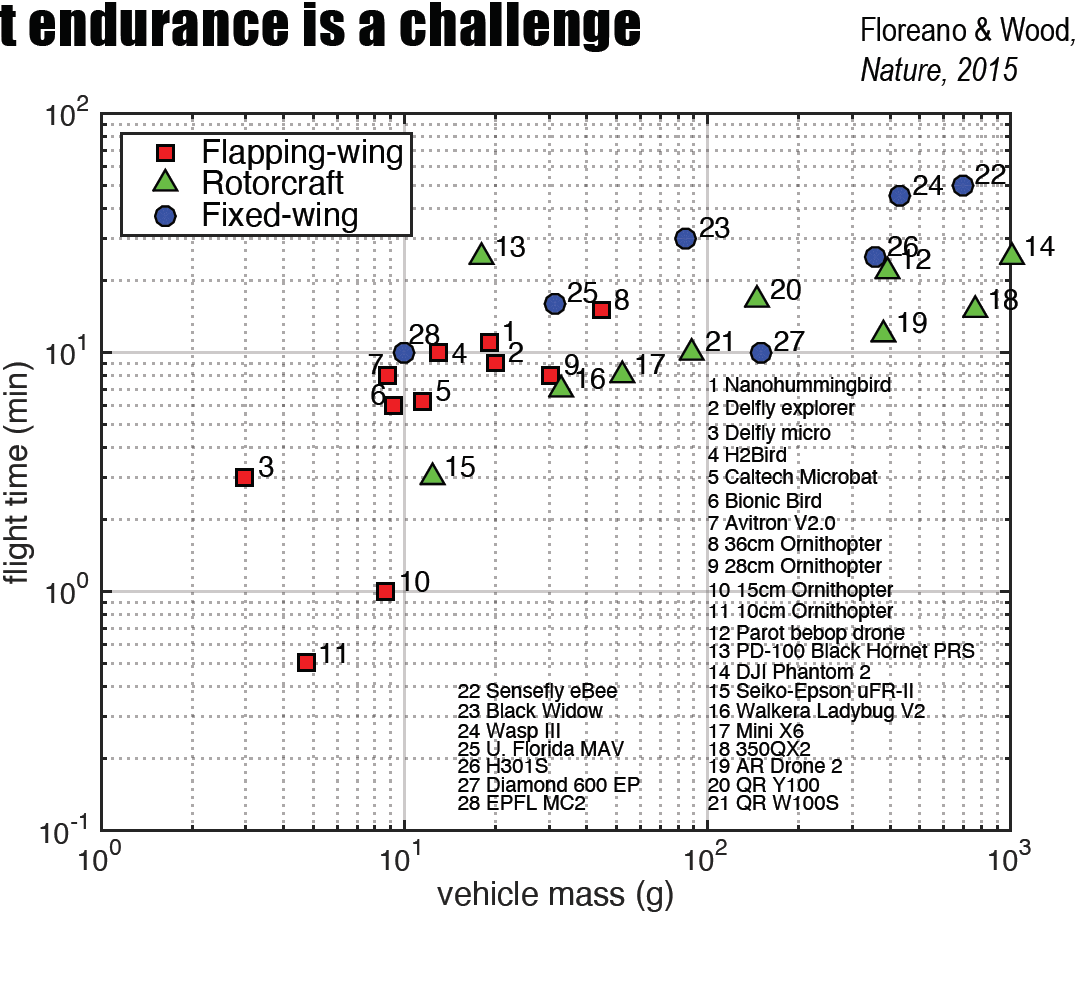
\includegraphics{F:/\#\#\#Learning@EPFL/\#MasterSemester_21Spring/Notes4Review_21Spring/pics/aerial/week1_endurance_mass.png}
  \caption{week1\_endurance\_mass}
  \end{figure}
\end{itemize}

\subsection{Fixed wing Staying in the Air}\label{header-n22}

generate a force \textbf{Lift} L equal and \textbf{opposite} to its own
\textbf{weight} W

\begin{figure}
\centering
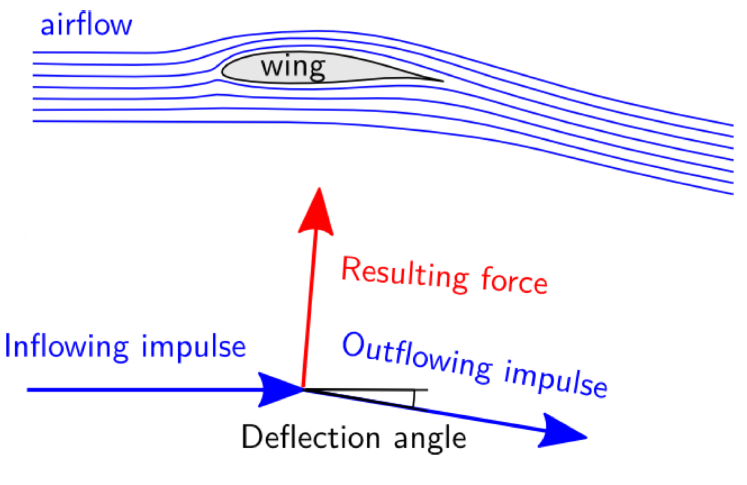
\includegraphics{F:/\#\#\#Learning@EPFL/\#MasterSemester_21Spring/Notes4Review_21Spring/pics/aerial/week1_hovering.png}
\caption{week1\_hovering}
\end{figure}

fixed-wing generates by airflow

\begin{itemize}
\item
  computing \textbf{lift}:
  \(W=\frac{1}{2} C^{l} * \rho {*} V^{2} * S \approx 0.3 * 1.25 * V^2 * S\)
  (sea level)

  \begin{itemize}
  \item
    lift coefficient \(C^{l}\): proportional to angle of attack

    at cruise speed \(6^{\circ}\), assuming \(\frac{1}{2} C^{l}= 0.2\) 
  \item
    Air density: decreases with the altitude

    1.25 \(kg/m^3\) at sea level
  \item
    Air speed V: fly 2x as fast -\textgreater{} 4x lift
  \item
    Wing area S
  \end{itemize}
\item
  compute the required \textbf{velocity} \(V = \sqrt{(W / 0.38 * S)}\)
\item
  Speed is proportional only to \textbf{wing loading} W/S
  \(W/S = 0.38V^2\)
\end{itemize}

\subsection{Maintaining constant speed V}\label{header-n44}

\begin{itemize}
\item
  generate a \textbf{thrust} force T equal and opposite to \textbf{Drag}
  force D
\item
  Drag \(D=\frac{1}{2} C^{d} * \rho {*} V^{2} * S = \rm{Lift}/r \)

  lift-drag ratio \(r = Lift/Drag\)
\end{itemize}

\subsection{Major Application Fields}\label{header-n51}

\begin{itemize}
\item
  Agriculture
\item
  Energy
\item
  Public safety \& security
\item
  Delivery
\end{itemize}

\subsubsection{For Agriculture}\label{header-n61}

\begin{itemize}
\item
  fixed-wing

  inspection: large fields; few lights/value
\item
  quadcopter

  spraying: small fields; high-value crops; difficult terrain
\end{itemize}

\subsubsection{For Energy}\label{header-n69}

\begin{itemize}
\item
  stationary inspection

  fire, related to human safety
\item
  long-range inspection

  frequent, faster inspection to powerline, gasoline
\item
  Power generation

  strong \& steady winds
\end{itemize}

\subsubsection{For Public safety \& security}\label{header-n80}

\begin{itemize}
\item
  in-vehicle

  policeman
\item
  long-range

  \textbf{Border} patrol, fast intervention
\end{itemize}

\subsubsection{For Delivery}\label{header-n88}

\paragraph{Category}\label{header-n89}

\begin{itemize}
\item
  Long-range: fixed wing; combination of wing and rotors to cover long
  distance
\item
  Short-range: multicopter
\end{itemize}

Forecast: parcel delivery \textgreater{} air freight in near future

\paragraph{«Can Drones Deliver?»}\label{header-n96}

\begin{itemize}
\item
  Power requirement: 0.59kW

  deliver 2 kg payload at cruising speed of 45 km/h
\item
  Energy requirement: about 0.39kWh

  deliver 2 kg payload within 10 km radius with 30 km/h headwind

  \begin{itemize}
  \item
    power (kW) x distance to speed ratio (d/v) to get energy requirement
    (kWh)
  \end{itemize}
\item
  Battery \& Platform: choose considerations -\textgreater{} cost;
  weight; energy density; lifetime
\item
  Economics: Electricity/Battery cost per km
\end{itemize}

\paragraph{\texorpdfstring{Last-cm delivery -
\href{https://dronistics.epfl.ch/}{Dronistics}}{Last-cm delivery - Dronistics}}\label{header-n111}

\begin{itemize}
\item
  PackDrone + SimplyFly

  Protective foldable cage; Redundant GPS
\item
  Temperature-control box for medicals
\end{itemize}

\subsection{☑️ Checkpoints}\label{header-n118}

\begin{itemize}
\item
  For a given total mass, what type of small drones (multi-copter,
  fixed-wing, flapping wing) displays the longest endurance?

  fixed-wing

  \begin{quote}
  fixed-wing drones generate lift with their wings. This means that,
  unlike a multirotor drone, they don't expend large amounts of energy
  just to stay in the air and fly more efficiently as a result
  \end{quote}
\item
  How much faster must an intercontinental airplane fly at cruising
  altitude compared to sea level?

  \(W=\frac{1}{2} C^{l} * \rho {*} V^{2} * S \rightarrow V = \sqrt{\frac{2W}{C^l \rho S}}\)

  \begin{itemize}
  \item
    sea level: \(\rho = 1.25kg/m^3\)
  \item
    intercontinental airplane fly \textasciitilde{}10000m:
    \(\rho = 0.4135kg/m^3\)
  \end{itemize}

  \(V \propto \sqrt{1/\rho}\)
\item
  What structural factor (i.e. not the engine) affects the cruising
  speed of fixed-wing drones?

  \sout{Speed is only proportional to wing loading (W/S) = Weight/Wing
  area}

  \begin{itemize}
  \item
    wing angle -\textgreater{} lift coefficient
  \item
    wing area
  \end{itemize}
\item
  What are the two major drone applications in agriculture?

  Inspection and spraying
\item
  What are the drone applications in the energy sector?

  Stationary inspection; long-range inspection; and power generation
\item
  What are the factors to consider for calculating the cost/km of drone
  delivery?

  Electricity cost and battery cost
\end{itemize}

\section{Multicopters (week1)}\label{header-n151}

\begin{longtable}[]{@{}llll@{}}
\toprule
& Fixed wing & Flapping wing & rotating wing\tabularnewline
\midrule
\endhead
\textbf{Examples} & airplanes, gliders & new robots & helicopters,
multicopters\tabularnewline
\textbf{Pros} & Fast; Efficient & Efficient & Can hover; Highly
maneuverable\tabularnewline
\textbf{Cons} & Cannot Hover & Hard to build and control & Less
efficient\tabularnewline
\textbf{Features} & & Scale down in size & Vertical take-off and landing
(VTOL)\tabularnewline
\bottomrule
\end{longtable}

\subsection{Introduction}\label{header-n178}

\subsubsection{Rotorcrafts (helicopters vs
multicopters)}\label{header-n179}

\begin{quote}
generates lift using high speed rotary blades called rotors
\end{quote}

\begin{itemize}
\item
  Features

  \begin{itemize}
  \item
    Vertical take-off and landing (VTOL)
  \item
    Very maneuverable
  \item
    Less efficient than fixed wing vehicle
  \end{itemize}
\item
  helicopters-Need complex variable pitch rotors

  \begin{itemize}
  \item
    the tail produce a moment to counteract the force generated by main
    propeller blade when generating main lift
  \item
    change the pitch of the blades (force vector) to produce
    translation-add complexity
  \end{itemize}
\item
  multicopters-Use multiple fixed-pitch blades

  \begin{itemize}
  \item
    each spin in different directions; don't need tails due to balanced
    moment
  \item
    fix pitch propellers 
  \end{itemize}

  \begin{quote}
  overtaken by helicopters due to heavy workload of the pilot
  \end{quote}
\end{itemize}

\subsubsection{Pros and Cons}\label{header-n208}

\paragraph{Pros-Easy to build and maintain}\label{header-n209}

\begin{itemize}
\item
  Mechanically simple
\item
  Does not require any complex mechanical parts
\item
  Can move around by changing motor speed
\item
  Can hover, takeoff, and land vertically
\end{itemize}

\paragraph{Cons}\label{header-n219}

\begin{itemize}
\item
  Required energy constantly to hover
\item
  \textbf{less efficient} than helicopters of the same size because the
  \textbf{thrust is generated by smaller propellers}.
\end{itemize}

\subsection{Structure and Physics}\label{header-n225}

\subsubsection{Main components}\label{header-n226}

frame; control board; Motors and motor drivers (ESC, electronic speed
controller); Propellers; Battery; Receiver

\subsubsection{Configuration}\label{header-n228}

\begin{itemize}
\item
  Four propellers generate four lift forces
\item
  Propellers 1\& 2 (CCW) have opposite pitch compared to propellers 3 \&
  4 (CW)

  \begin{figure}
  \centering
  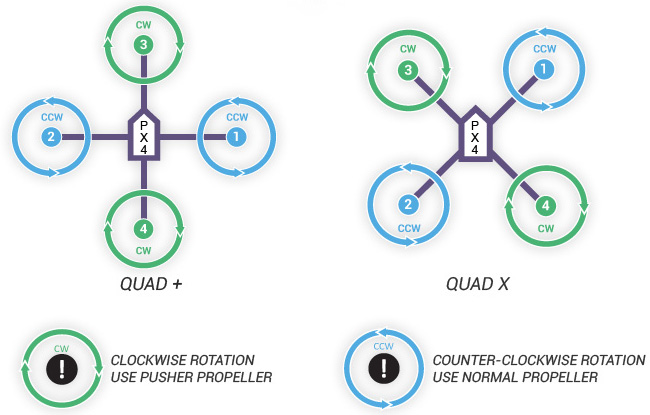
\includegraphics{F:/\#\#\#Learning@EPFL/\#MasterSemester_21Spring/Notes4Review_21Spring/pics/aerial/week1_frame.png}
  \caption{week1\_frame}
  \end{figure}
\end{itemize}

\subsubsection{Rotation speeds / Forces / Moments}\label{header-n235}

\begin{quote}
movement are controlled by changing the rotation speed of the propellers
\end{quote}

\begin{itemize}
\item
  Force F is \textbf{proportional to square of} propeller \textbf{speed}
  \(F_i \propto w_i^2\)
\item
  mg is the \textbf{weight} of the quadrotor
\item
  \textbf{Moments} generated by the forces are \(M_i = L \propto F_i\)
\end{itemize}

\begin{figure}
\centering
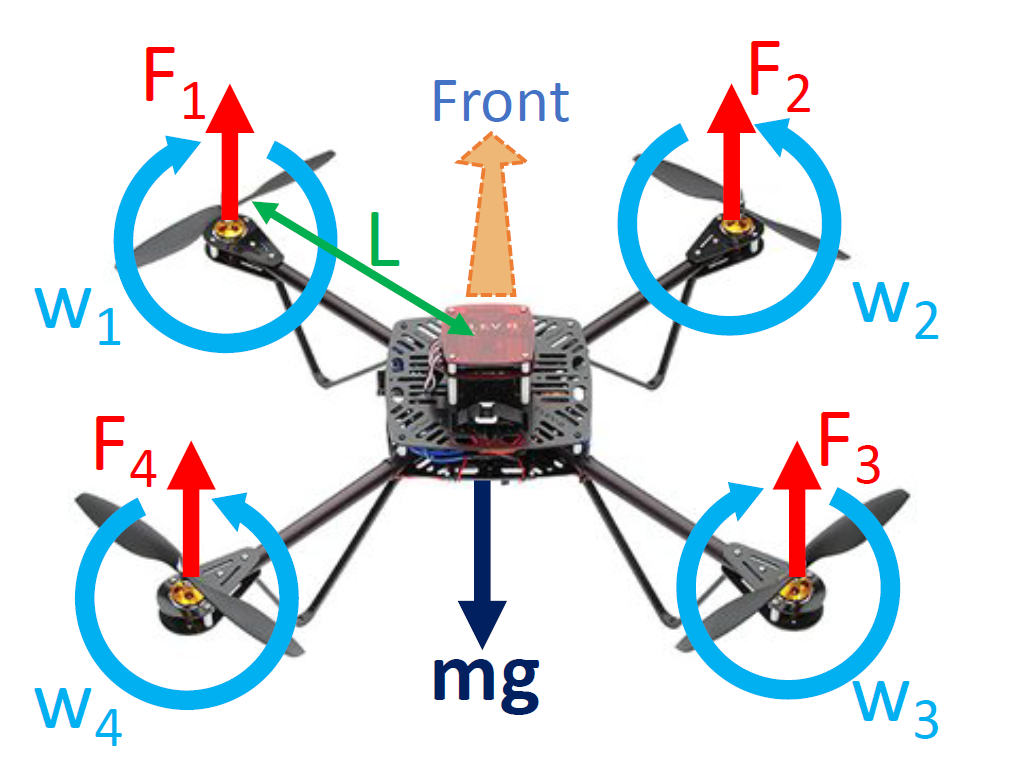
\includegraphics{F:/\#\#\#Learning@EPFL/\#MasterSemester_21Spring/Notes4Review_21Spring/pics/aerial/week1_force.png}
\caption{week1\_force}
\end{figure}

\subsubsection{Hover conditions}\label{header-n246}

\begin{enumerate}
\def\labelenumi{\arabic{enumi}.}
\item
  All forces must be balanced \(F_1+ F_2+ F_3+ F_4+ mg = 0\)

  move up and down
\item
  Lift forces must be parallel to gravity \(F_i \Vert g\)
\item
  All moments must be balanced \(M_1+M_2+M_3+M_4 = 0\)

  pitch and roll
\item
  Rotor speeds must be balanced (torque balanced) \((w1+w3)-(w2+w4) =0\)

  yaw
\end{enumerate}

\subsection{Flight mechanics}\label{header-n259}

\begin{quote}
How to move a quadrotor around?
\end{quote}

\begin{itemize}
\item
  \textbf{Orientation}

  \begin{figure}
  \centering
  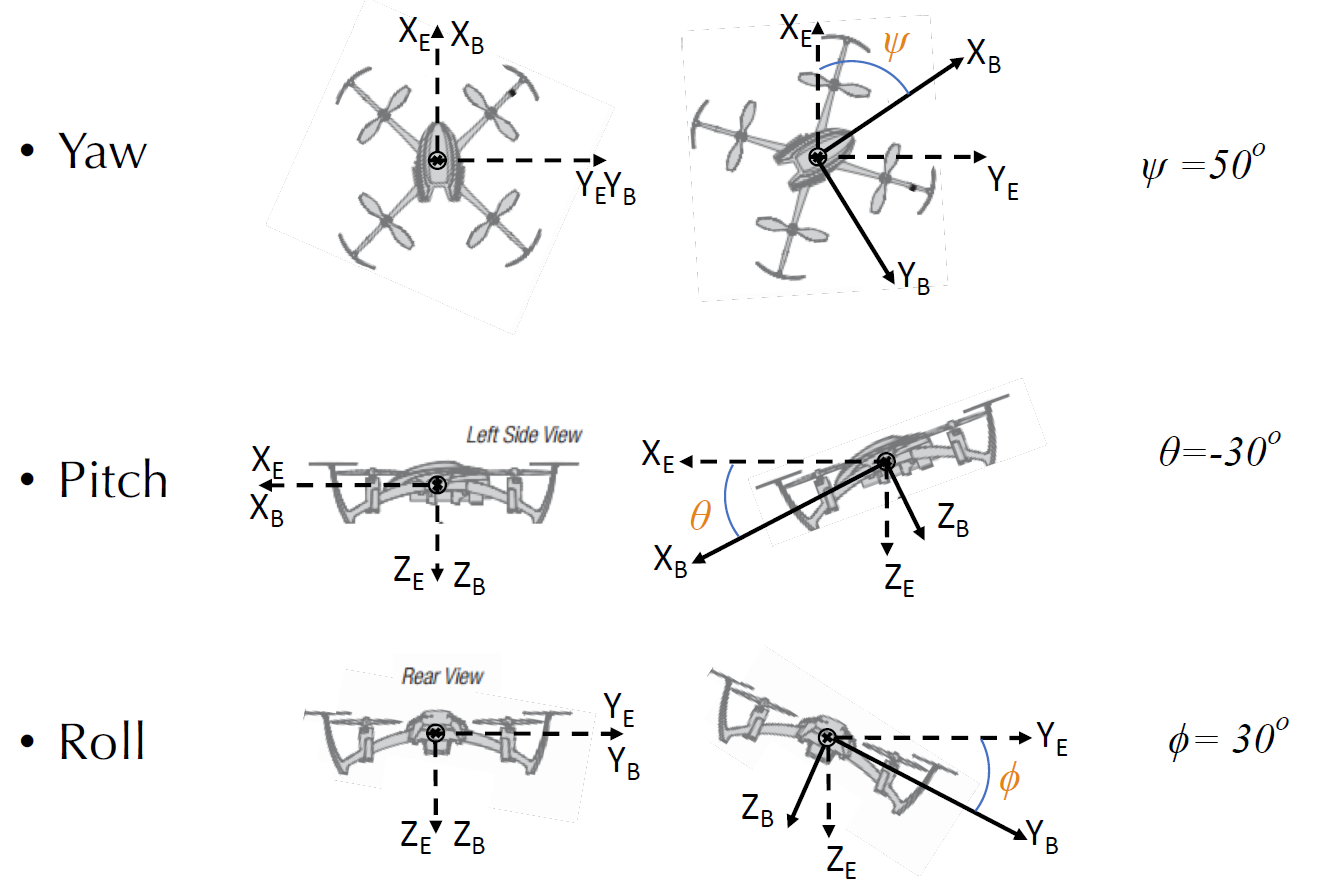
\includegraphics{F:/\#\#\#Learning@EPFL/\#MasterSemester_21Spring/Notes4Review_21Spring/pics/aerial/week1_rpy.png}
  \caption{week1\_rpy}
  \end{figure}
\end{itemize}

\begin{quote}
Violating one or more of these conditions implies that \textbf{the
quadcopter starts to move}
\end{quote}

\subsubsection{Moving Up and Down}\label{header-n269}

\begin{itemize}
\item
  \textbf{condition1}: Forces Not balanced
  \(F_1+ F_2+ F_3+ F_4+ mg \neq 0\)
\end{itemize}

\subsubsection{Rotating in Yaw}\label{header-n273}

\begin{figure}
\centering
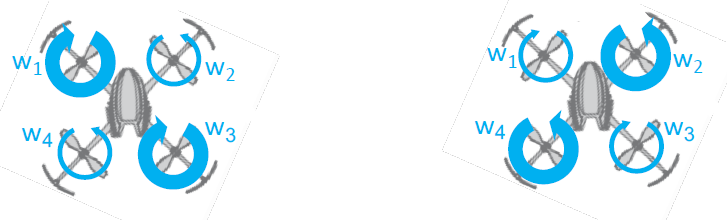
\includegraphics{F:/\#\#\#Learning@EPFL/\#MasterSemester_21Spring/Notes4Review_21Spring/pics/aerial/week1_rollpitch.png}
\caption{week1\_rollpitch}
\end{figure}

\begin{itemize}
\item
  Rotor speeds not balanced (torque balanced) \((w1+w3)-(w2+w4) \neq 0\)

  \(\dot{\psi}=k_{\psi}\left(\left({w}_{2}+{w}_{4}\right)-\left({w}_{1}+{w}_{3}\right)\right)\)
\item
  Note: opposite motor pair should increase/decrease motor speeds to
  keep hovering, or it will keep flying up!
\end{itemize}

\subsubsection{Rotation in Roll/Pitch}\label{header-n281}

\begin{itemize}
\item
  Forces not parallel to gravity \(F_i \nparallel mg \)
\item
  moments not balanced \(M_1+M_2+M_3+M_4 \neq 0\)

  \(\dot{\phi}=k_{\phi}\left(\left(w_{1}+w_{4}\right)-\left(w_{2}+w_{3}\right)\right)\)

  \(\dot{\theta}=k_{\theta}\left(\left(w_{1}+w_{2}\right)-\left(w_{3}+w_{4}\right)\right)\)
\end{itemize}

\subsubsection{Summary of equations}\label{header-n289}

\begin{figure}
\centering
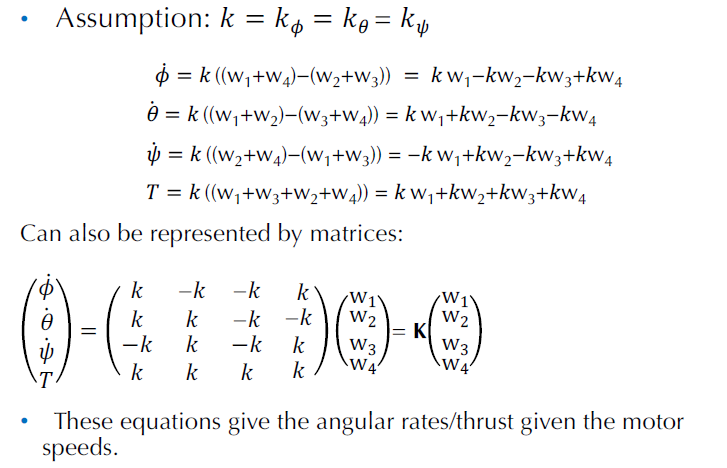
\includegraphics{F:/\#\#\#Learning@EPFL/\#MasterSemester_21Spring/Notes4Review_21Spring/pics/aerial/week1_speed2motion.png}
\caption{week1\_speed2motion}
\end{figure}

\begin{itemize}
\item
  to control the quadrotor state -\textgreater{} setting the rotor
  speeds for obtaining a desired angular rotation

  \textbf{inverse} operation
\end{itemize}

\subsubsection{Example-Translated flight}\label{header-n295}

\begin{quote}
Moving Forward

Translated flight \textbf{requires more thrust than hovering}, but not
always more power (see section 6)!
\end{quote}

\begin{itemize}
\item
  pitch down: decrease F\emph{1 and F}2
\item
  hover: increase F\emph{1 and F}2 to stop rotation
\item
  translate: keep balance between mg and thrust
  \(\mathbf{F} \cos \theta=-m g\)

  \begin{figure}
  \centering
  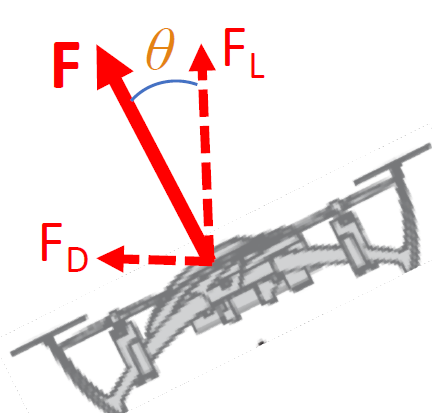
\includegraphics{F:/\#\#\#Learning@EPFL/\#MasterSemester_21Spring/Notes4Review_21Spring/pics/aerial/week1_move.png}
  \caption{week1\_move}
  \end{figure}
\item
  pitch back
\end{itemize}

\subsection{Types of Multicopters}\label{header-n309}

\begin{quote}
main feature; fully actuated multicopters
\end{quote}

\subsubsection{Configuration}\label{header-n312}

\begin{figure}
\centering
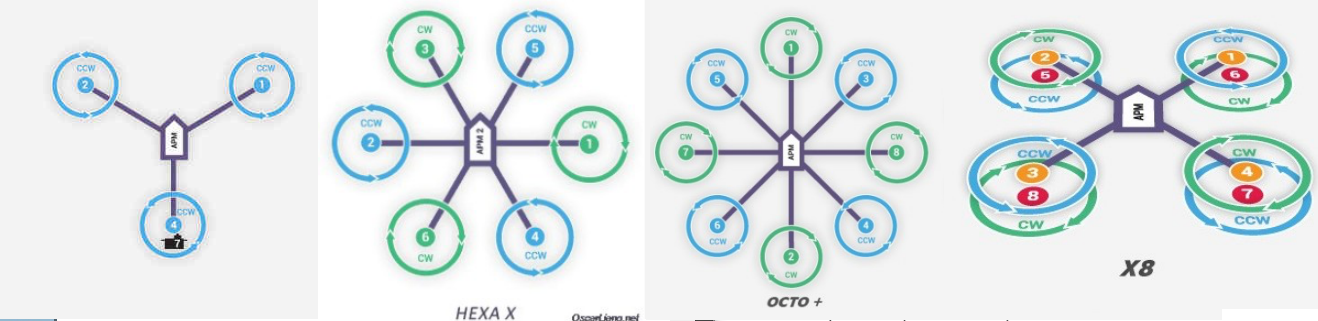
\includegraphics{F:/\#\#\#Learning@EPFL/\#MasterSemester_21Spring/Notes4Review_21Spring/pics/aerial/week1_config.png}
\caption{week1\_config}
\end{figure}

\begin{itemize}
\item
  Tricopter

  \begin{itemize}
  \item
    More yaw authority compared to quadcopters

    direct control of yaw
  \item
    More complex mechanical design due to the \textbf{servo} in tail

    need additional servo to roll/pitch the back motor
  \end{itemize}
\item
  Hexacopter/Octocopter

  \begin{itemize}
  \item
    More lifting capacity -\textgreater{} more payload
  \item
    \textbf{Redundancy}, so robust to failure
  \item
    Larger size; expensive
  \end{itemize}
\item
  X8 configuration

  \begin{itemize}
  \item
    More lifting capacity
  \item
    \textbf{More efficiency} thanks to the \textbf{coaxial
    configurations}
  \end{itemize}
\end{itemize}

\subsubsection{Fully Actuated Multicopters}\label{header-n340}

\begin{quote}
underactuated multicopters -\textgreater{} all propellers are rotated in
the same plane
\end{quote}

\paragraph{Features}\label{header-n343}

\begin{itemize}
\item
  Rotors disks are in different planes
\item
  Fully Actuated to control 6 DoF (heave, roll, pitch and yaw, x and y
  translation) by using 6 motors
\end{itemize}

\paragraph{Pros}\label{header-n349}

\begin{itemize}
\item
  Translational and rotational \textbf{dynamics} are \textbf{decoupled}
\item
  \textbf{improved robustness to disturbances} and to perform complex
  manipulation tasks
\item
  Possibility to plan \textbf{more complex trajectories}
\end{itemize}

\paragraph{Cons}\label{header-n357}

\begin{itemize}
\item
  Decreased energetic efficiency
\end{itemize}

\subsection{Energetics}\label{header-n361}

\begin{quote}
What is the power consumption of a multicopter during flight?

How to extend multicopters flight time?
\end{quote}

\begin{itemize}
\item
  Multicopters have high power requirements

  inefficient compared to fixed-wing or flapping-wing aircraft

  \begin{itemize}
  \item
    consume about 200 W/kg on average
  \item
    Centimeter scale quad with LiPo -\textgreater{} 5-7min
  \item
    Decimeter scale quad with LiPo -\textgreater{}20-30min

    changes corresponding to \textbf{weather conditions} and
    \textbf{aggressiveness of flight}
  \end{itemize}
\end{itemize}

\subsubsection{Energy in hovering}\label{header-n377}

\begin{figure}
\centering
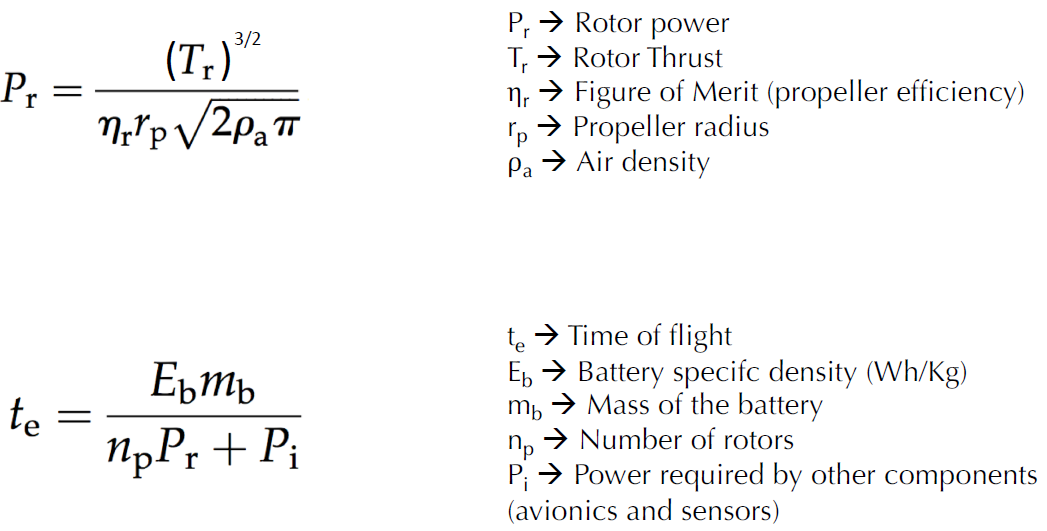
\includegraphics{F:/\#\#\#Learning@EPFL/\#MasterSemester_21Spring/Notes4Review_21Spring/pics/aerial/week1_energetics.png}
\caption{week1\_energetics}
\end{figure}

\begin{itemize}
\item
  Power calculation of single motor when drone in hovering

  \begin{itemize}
  \item
    Propeller efficiency ranges from 0.85 to about 0.9
  \item
    \(r_p \sqrt{\pi}\) is the squire root of the disk area
  \end{itemize}
\item
  Flight time

  \begin{itemize}
  \item
    \(P_i\) has high variability
  \end{itemize}
\end{itemize}

\subsubsection{Energy in forward flight of
quadcopter}\label{header-n392}

\begin{itemize}
\item
  Power consumption during forward flight normalized by the power
  consumption at hover

  \begin{figure}
  \centering
  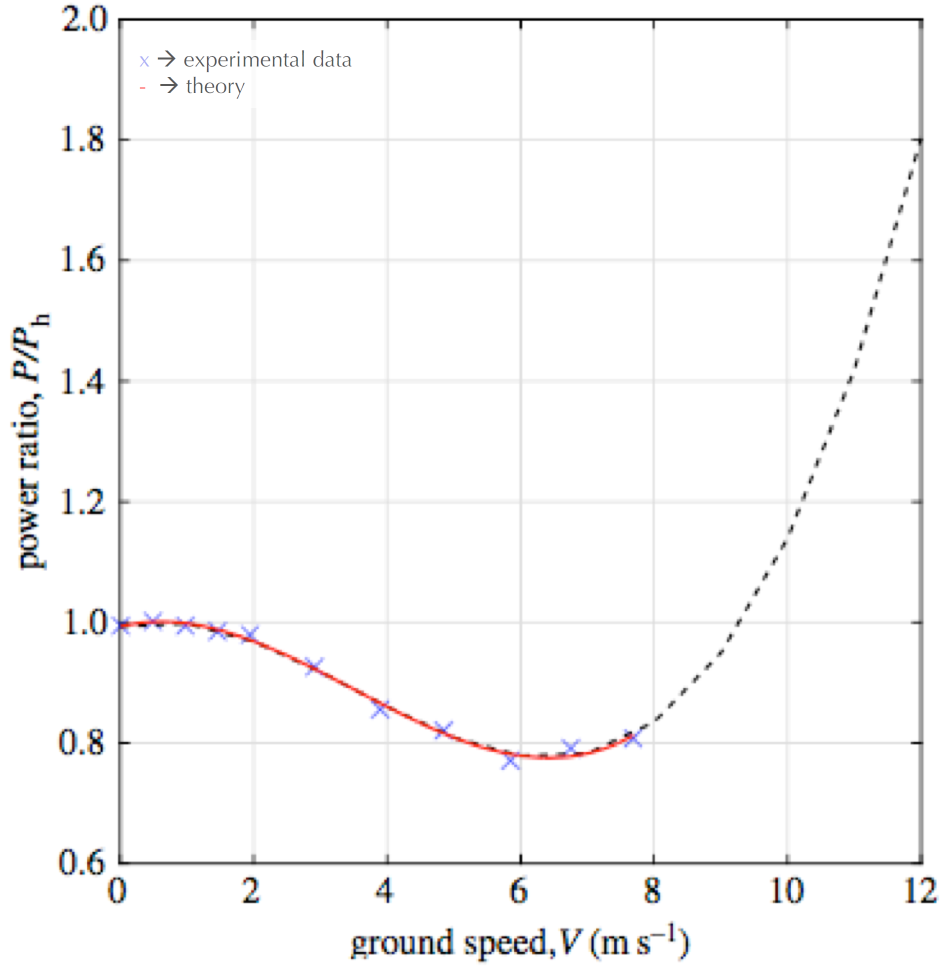
\includegraphics{F:/\#\#\#Learning@EPFL/\#MasterSemester_21Spring/Notes4Review_21Spring/pics/aerial/week1_translation_flight.png}
  \caption{week1\_translation\_flight}
  \end{figure}

  \begin{itemize}
  \item
    lower power need but higher thrust -\textgreater{} aerodynamics

    tilting the quad to the side -\textgreater{} \textbf{artificially
    increase the angle of attack -\textgreater{} generate the increase
    in thrust in the given power}
  \item
    high power ratio again

    drag increases quickly again!
  \end{itemize}
\end{itemize}

\subsubsection{Increase flight time}\label{header-n404}

\begin{enumerate}
\def\labelenumi{\arabic{enumi}.}
\item
  Weight and drag reduction
\item
  Increase the specific power of the energy source

  switch from LiPo batteries to gasoline (far more energy stored)
\item
  Docking station for charging/battery swapping
\item
  Tether for power supply

  reduce battery
\item
  Improving efficiency via mechanical
\item
  Energy aware motion planning

  reduce acceleration (aggressive flight)
\item
  Multi-modal operation

  perching; walking and rolling
\end{enumerate}

\subsection{☑️ Checkpoints}\label{header-n424}

\begin{itemize}
\item
  What set of conditions corresponds to hovering in a quadcopter?

  Four conditions: balanced weight; parallel to weight; balanced moment
  (thrust x half frame); balanced rotation speed
\item
  What set of conditions corresponds to a rotation around the yaw axis
  in a quadcopter?

  imbalanced rotation speed
\item
  How the time of flight of multicopters can be increased?

  \begin{enumerate}
  \def\labelenumi{\arabic{enumi}.}
  \item
    Weight and drag reduction
  \item
    Increase the specific power of the energy source
  \item
    Docking station for charging/battery swapping
  \item
    Tether for power supply
  \item
    Improving efficiency via mechanical
  \item
    Energy aware motion planning
  \item
    Multi-modal operation
  \end{enumerate}
\item
  How the power consumption and total thrust evolve at different forward
  speeds in multicopters?

  first goes down as thus increases when angle of attack increases

  then goes down because the drag force increases again
\end{itemize}

\section{Attitude representations (week2)}\label{header-n453}

\begin{figure}
\centering
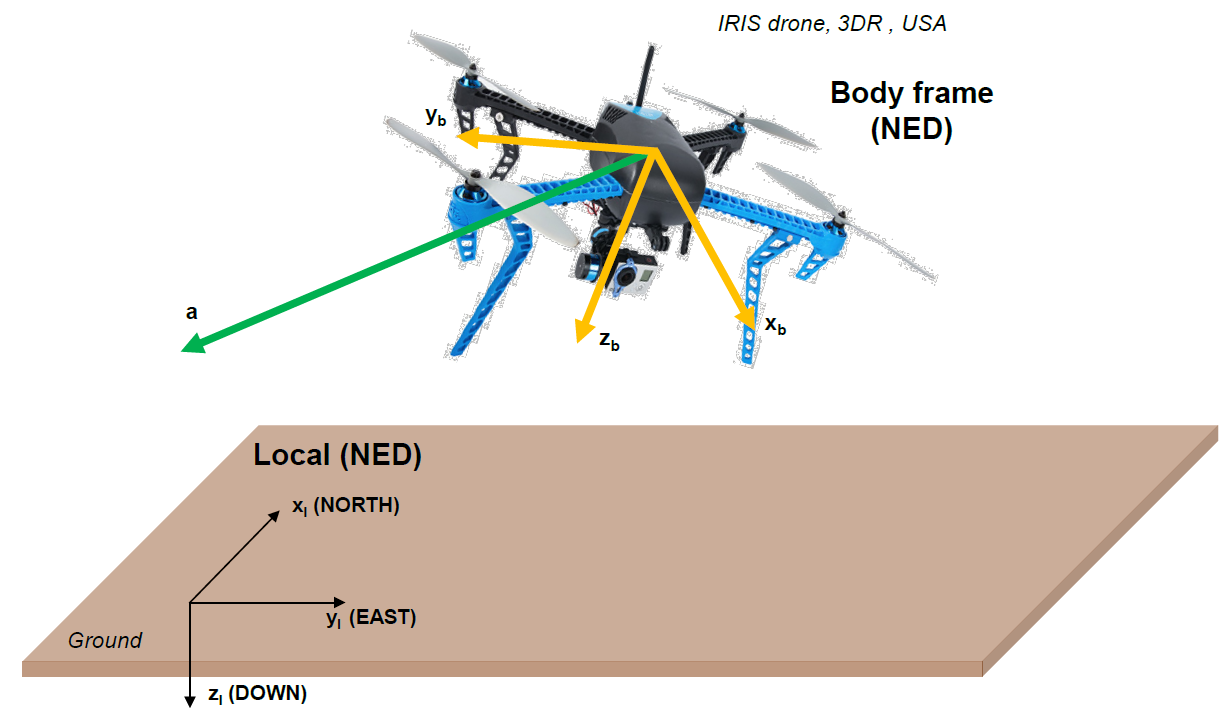
\includegraphics{F:/\#\#\#Learning@EPFL/\#MasterSemester_21Spring/Notes4Review_21Spring/pics/aerial/week2_frame.png}
\caption{week2\_frame}
\end{figure}

\begin{itemize}
\item
  how to convert state variables from body frame to earth frame
\end{itemize}

\subsection{3D Attitude representation- Euler Angles}\label{header-n458}

\begin{itemize}
\item
  Rotation matrices can be parametrize by Euler Angles

  \begin{itemize}
  \item
    Roll \(\phi\): rotation around x
  \item
    Pitch \(\theta\): rotation around y
  \item
    Yaw \(\psi\): rotation around z
  \end{itemize}

  \begin{figure}
  \centering
  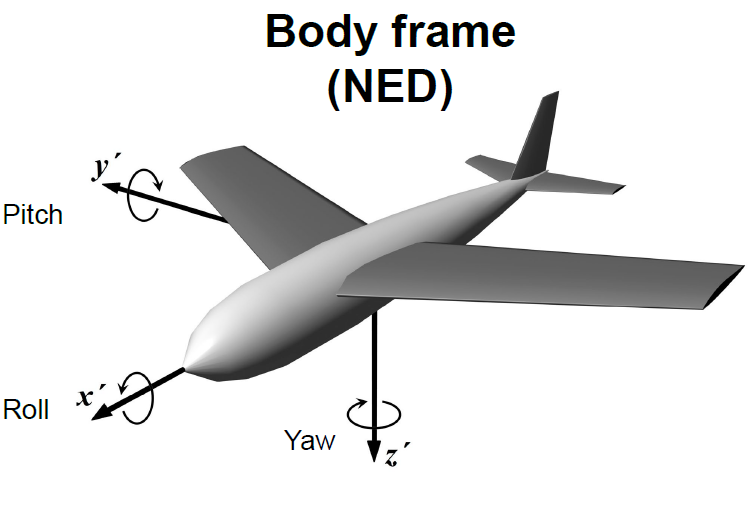
\includegraphics{F:/\#\#\#Learning@EPFL/\#MasterSemester_21Spring/Notes4Review_21Spring/pics/aerial/week2_euler.png}
  \caption{week2\_euler}
  \end{figure}
\item
  Yaw-Pitch-Roll rotation matrix (Z,Y,X) or Heading-Pitch-Roll (h-p-r)

  \begin{figure}
  \centering
  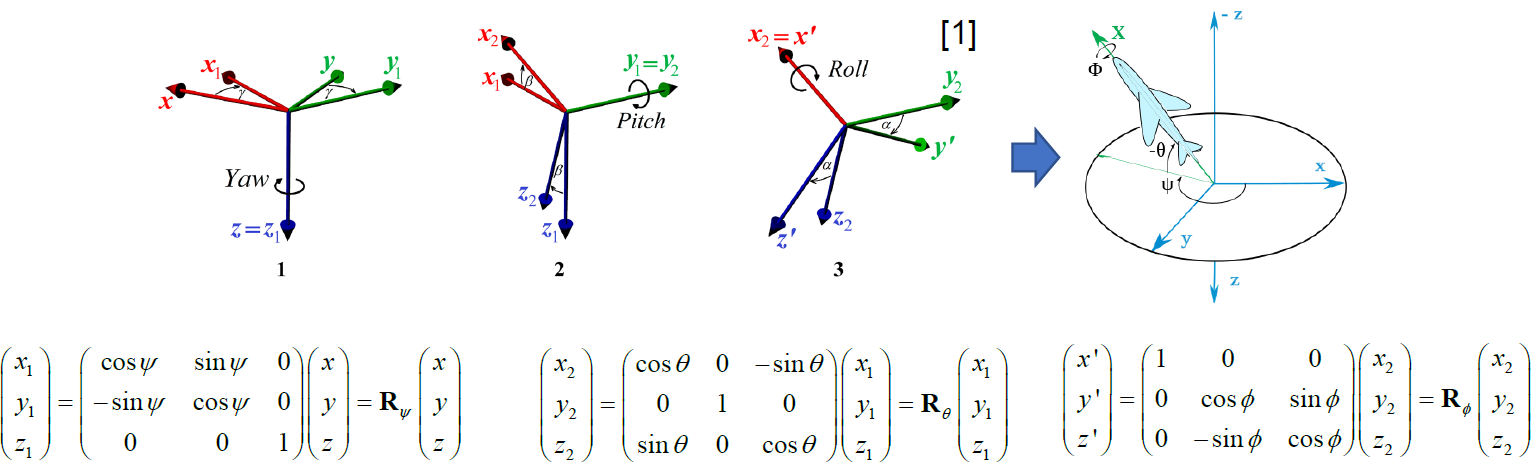
\includegraphics{F:/\#\#\#Learning@EPFL/\#MasterSemester_21Spring/Notes4Review_21Spring/pics/aerial/week2_euler_ypr.png}
  \caption{week2\_euler\_ypr}
  \end{figure}

  can be summarized as \(R=R_{\phi} R_{\theta} R_{\psi}\) (左乘)
\item
  🚧 Claw Example

  rotation + translation

  补充示例!!!
\item
  Issues: gimbal lock problem

  \begin{itemize}
  \item
    sensitive to singularities-when pitch angle is 90 degrees,
    \textbf{roll and yaw} \textbf{rotations give the same sensor
    readings}

    lost 1 DoF

    \(R=R_{\phi} R_{\frac{\pi}{2}} R_{\psi}=\left[\begin{array}{ccc}0 & 0 & -1 \\ \sin \phi \cos \psi-\cos \phi \sin \psi & \sin \phi \sin \psi+\cos \phi \cos \psi & 0 \\ \cos \phi \cos \psi+\sin \phi \sin \psi & \cos \phi \sin \psi-\sin \phi \cos \psi & 0\end{array}\right]=\)
    \(\left[\begin{array}{ccc}0 & 0 & -1 \\ \sin (\phi-\psi) & \cos (\phi-\psi) & 0 \\ \cos (\phi-\psi) & -\sin (\phi-\psi) & 0\end{array}\right]\)
  \item
    \textbf{fail to produce reliable estimates} when the pitch angle
    approaches 90 degrees.
  \item
    can only be solved by \textbf{switching to a different
    representation} methods, for example \textbf{quaternions}
  \end{itemize}
\end{itemize}

\subsection{Quaternion}\label{header-n489}

\begin{quote}
the union of scalar and vector
\end{quote}

\begin{figure}
\centering
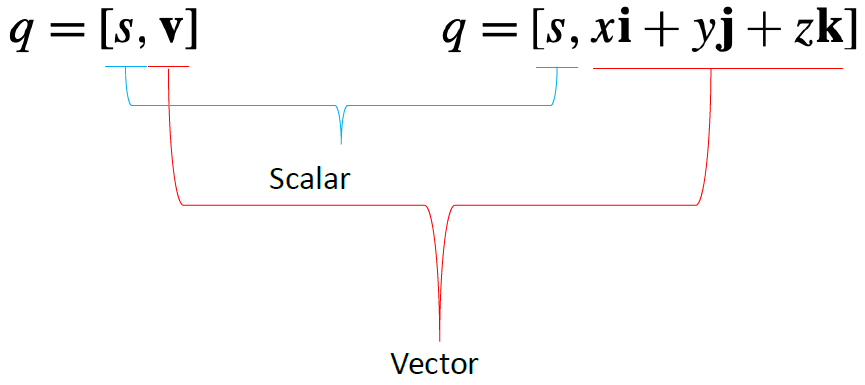
\includegraphics{F:/\#\#\#Learning@EPFL/\#MasterSemester_21Spring/Notes4Review_21Spring/pics/aerial/week2_quaternion.png}
\caption{week2\_quaternion}
\end{figure}

\begin{itemize}
\item
  rotation vector = quet * vector * quet\^{}(-1)

  \begin{figure}
  \centering
  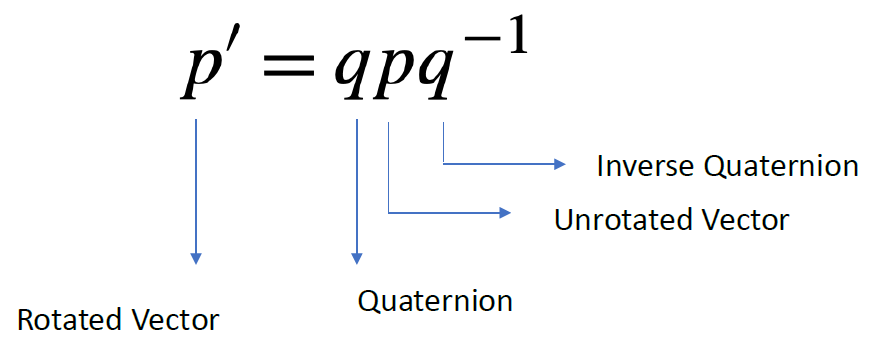
\includegraphics{F:/\#\#\#Learning@EPFL/\#MasterSemester_21Spring/Notes4Review_21Spring/pics/aerial/week2_rotata_quet.png}
  \caption{week2\_rotata\_quet}
  \end{figure}

  \begin{itemize}
  \item
    \( p = [0, \mathbf{p}]\) vector in 3-space
  \item
    \(q = [s, \lambda \hat{\mathbf{v}}]\) Must meet these requirements

    $\vert \hat{\mathbf{v}} \vert = 1$; \(s^2 + \lambda^2 = 1\)
  \end{itemize}
\item
  multiplication

  \begin{figure}
  \centering
  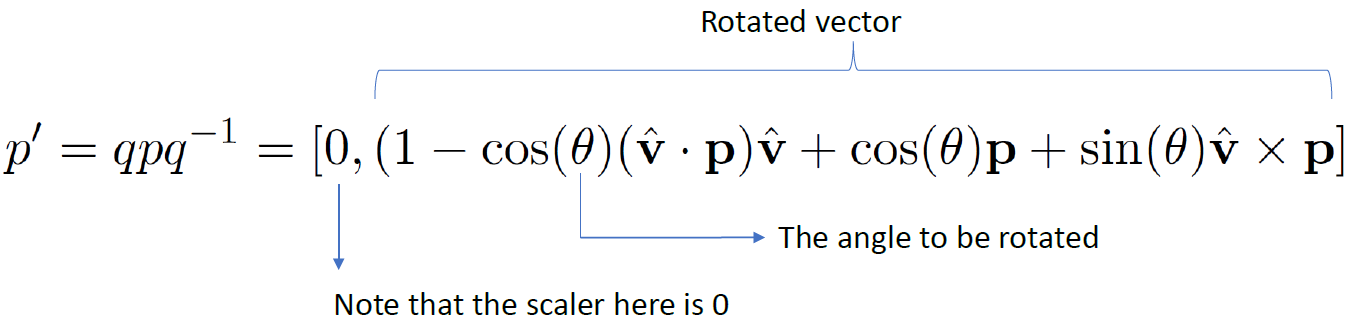
\includegraphics{F:/\#\#\#Learning@EPFL/\#MasterSemester_21Spring/Notes4Review_21Spring/pics/aerial/week2_euler_mul.png}
  \caption{week2\_euler\_mul}
  \end{figure}

  \(q=\left[\cos \frac{1}{2} \theta, \sin \frac{1}{2} \theta \hat{\mathbf{v}}\right]\)
  works for relative to x axis (\(\theta\))

  week2\emph{quaternion}mat.png

  \begin{figure}
  \centering
  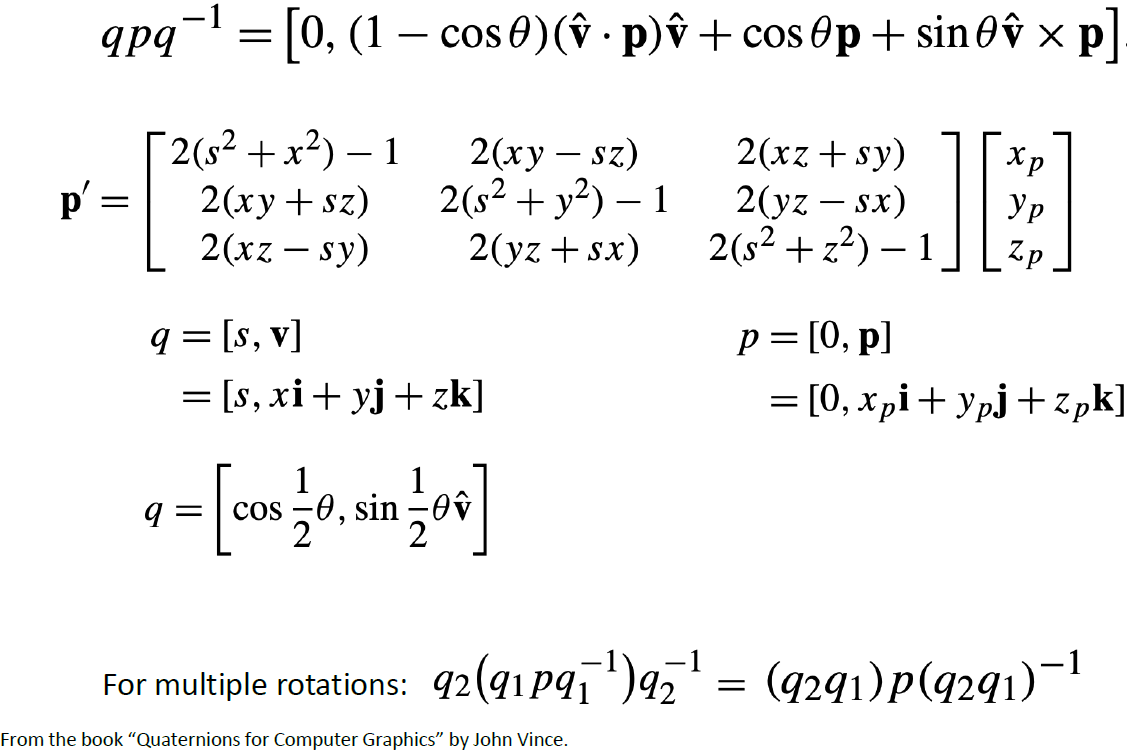
\includegraphics{F:/\#\#\#Learning@EPFL/\#MasterSemester_21Spring/Notes4Review_21Spring/pics/aerial/week2_quaternion_mat.png}
  \caption{week2\_quaternion\_mat}
  \end{figure}
\end{itemize}

\textbf{🚧 Claw Example}

rotation + translation using quaternions

\subsubsection{Conversion}\label{header-n511}

\begin{itemize}
\item
  Euler angles to quaternion
\item
  Quaternion to Euler angles (arctan2 is recommended)
\end{itemize}

\subsection{Complex examples}\label{header-n517}

\begin{quote}
frame: image/centered -\textgreater{} camera -\textgreater{} gimbal
-\textgreater{} body -\textgreater{} local
\end{quote}

\(v_{l}=p+R_{p}^{l} v_{p}=p+R_{b}^{l} R_{g}^{b} R_{c}^{g} R_{i}^{c} R_{p}^{i} v_{p}\)

\textbf{🚧 注意谁相对谁!!!}

\subsection{✖️ Checkpoints}\label{header-n522}

\begin{itemize}
\item
  nothing left in this course
\end{itemize}

\section{Control (week2\&3)}\label{header-n526}

\begin{quote}
结合exercise进行再次查看
\end{quote}

\subsection{Cascaded control Architecture}\label{header-n529}

\begin{itemize}
\item
  drone architecture

  \begin{figure}
  \centering
  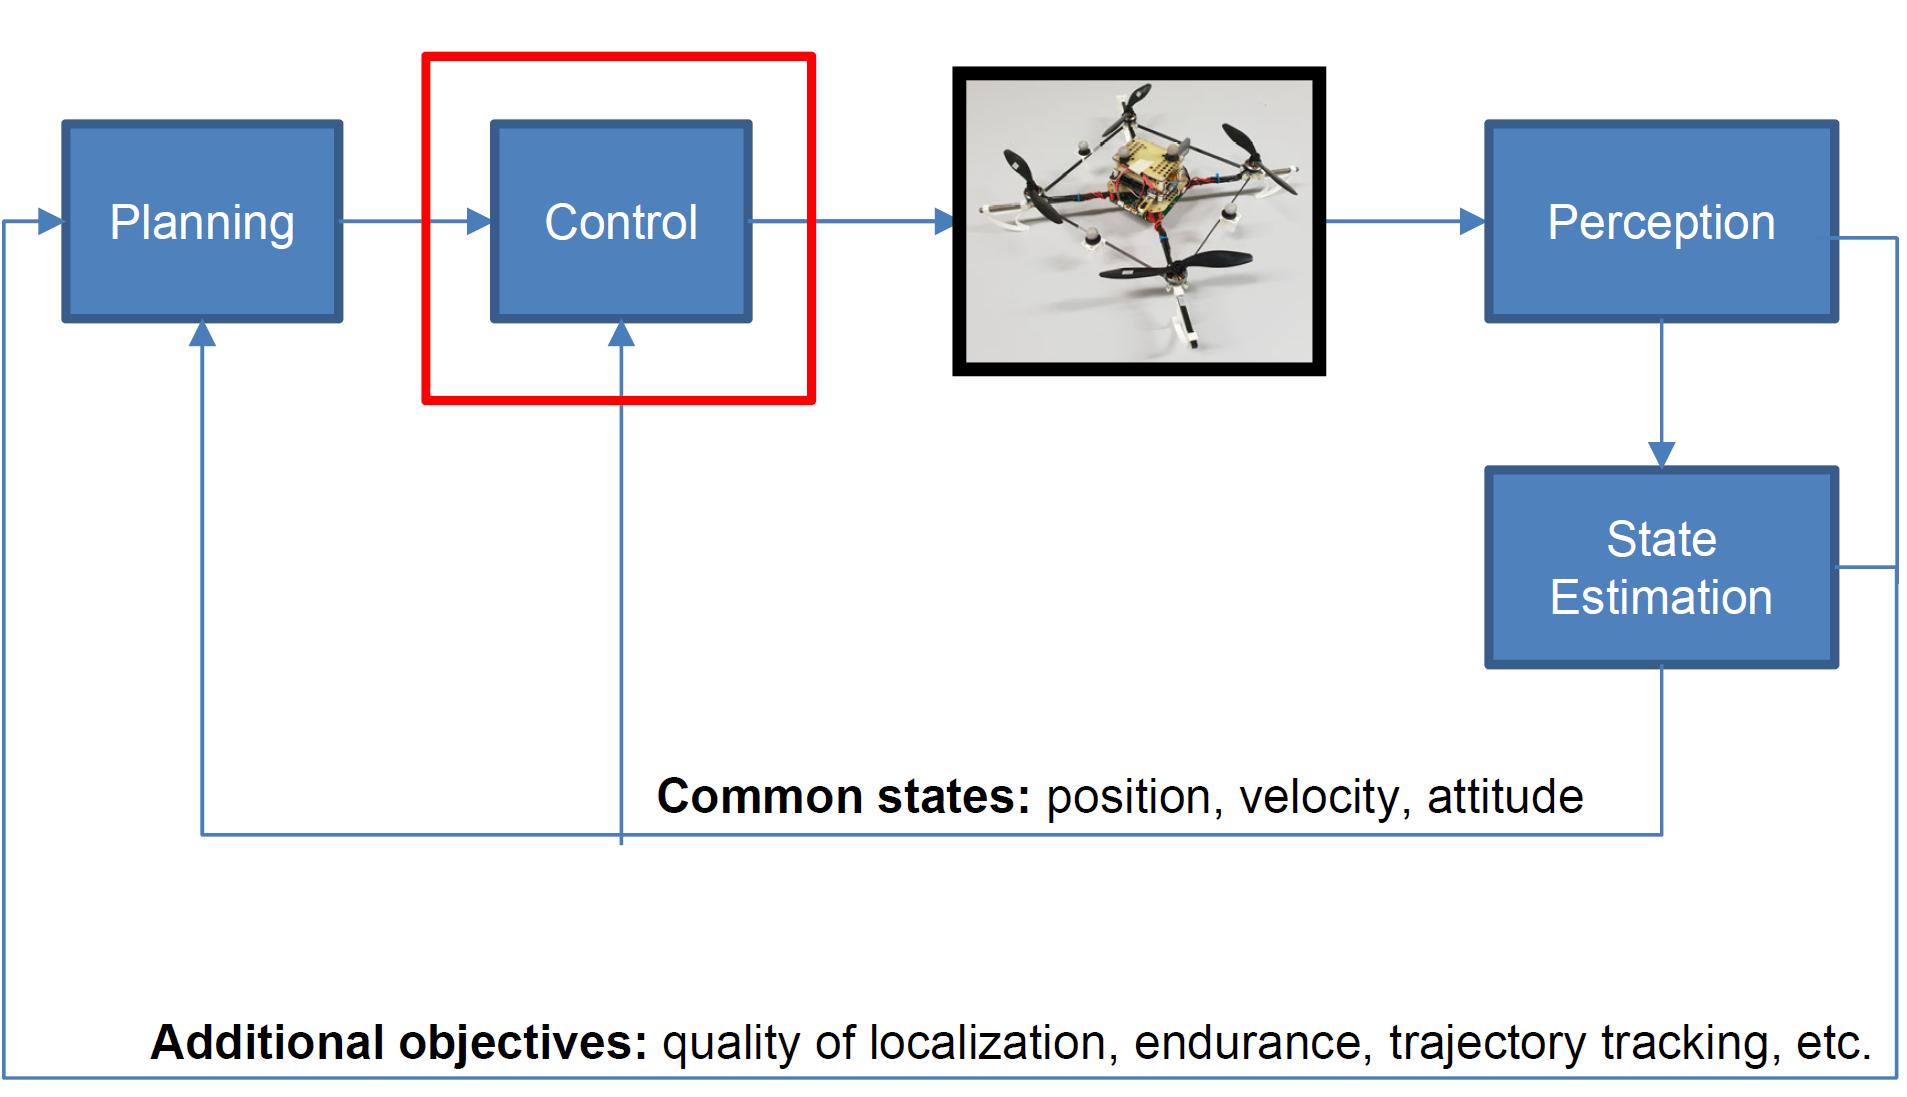
\includegraphics{F:/\#\#\#Learning@EPFL/\#MasterSemester_21Spring/Notes4Review_21Spring/pics/aerial/week2_control_diagram.png}
  \caption{week2\_control\_diagram}
  \end{figure}
\item
  communication: glue to connect different parts (FCU to onboard
  computer to ground station)
\item
  PID controller

  \begin{figure}
  \centering
  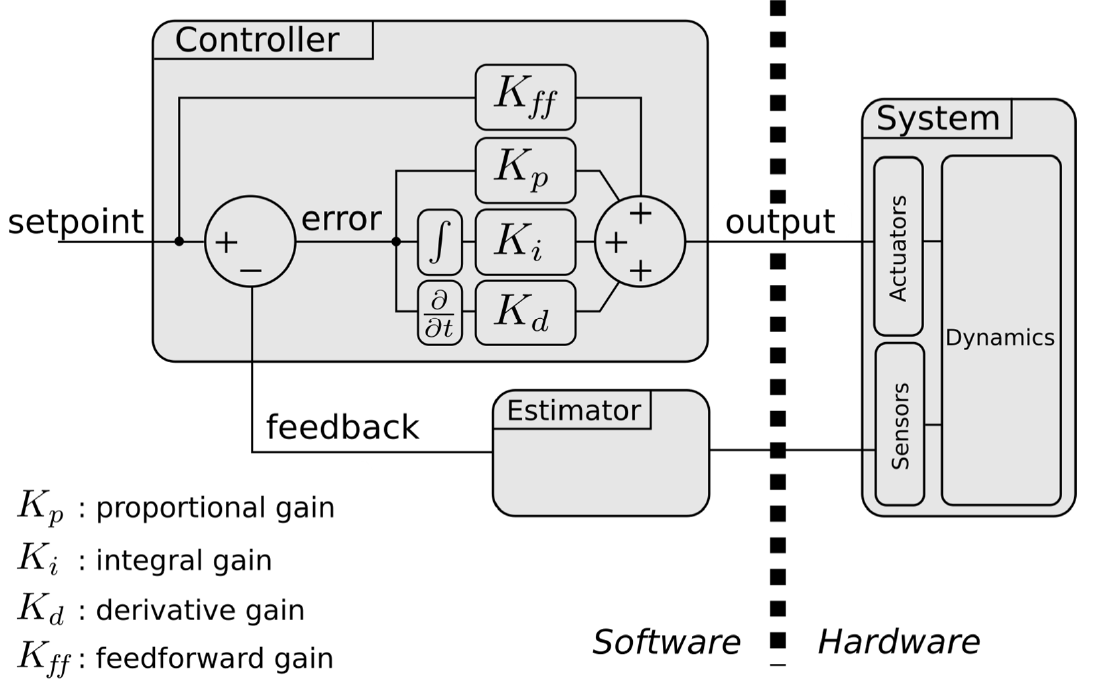
\includegraphics{F:/\#\#\#Learning@EPFL/\#MasterSemester_21Spring/Notes4Review_21Spring/pics/aerial/week2_pid.png}
  \caption{week2\_pid}
  \end{figure}

  \begin{itemize}
  \item
    Open-loop
  \item
    Feedforward control

    \begin{itemize}
    \item
      responds to its control signal in a \textbf{pre-defined way}
    \item
      based on a \textbf{previous knowledge} of the system
    \end{itemize}
  \item
    Feedback control
  \end{itemize}
\item
  control example

  \begin{longtable}[]{@{}lllll@{}}
  \toprule
  Examples & Free-flight glider & Passively stable helicopter & Racing
  drone & Autonomous Delivery drone\tabularnewline
  \midrule
  \endhead
  Sensors & None & None & IMU & IMU + GPS + Vision + Mag\tabularnewline
  Controllers & None & None & (Attitude), Rate & Position, Velocity,
  Attitude, Rate\tabularnewline
  Setpoint & None & Manual actuator setpoint & Manual rate setpoint &
  Autonomous navigation/Manual\tabularnewline
  \bottomrule
  \end{longtable}
\item
  challenges

  \begin{itemize}
  \item
    underactuated system for quadcopter
  \item
    approximate aerodynamic model
  \item
    control inputs are idealized (the \textbf{real model of the motors}
    can be quite hard to model)
  \end{itemize}
\end{itemize}

\begin{figure}
\centering
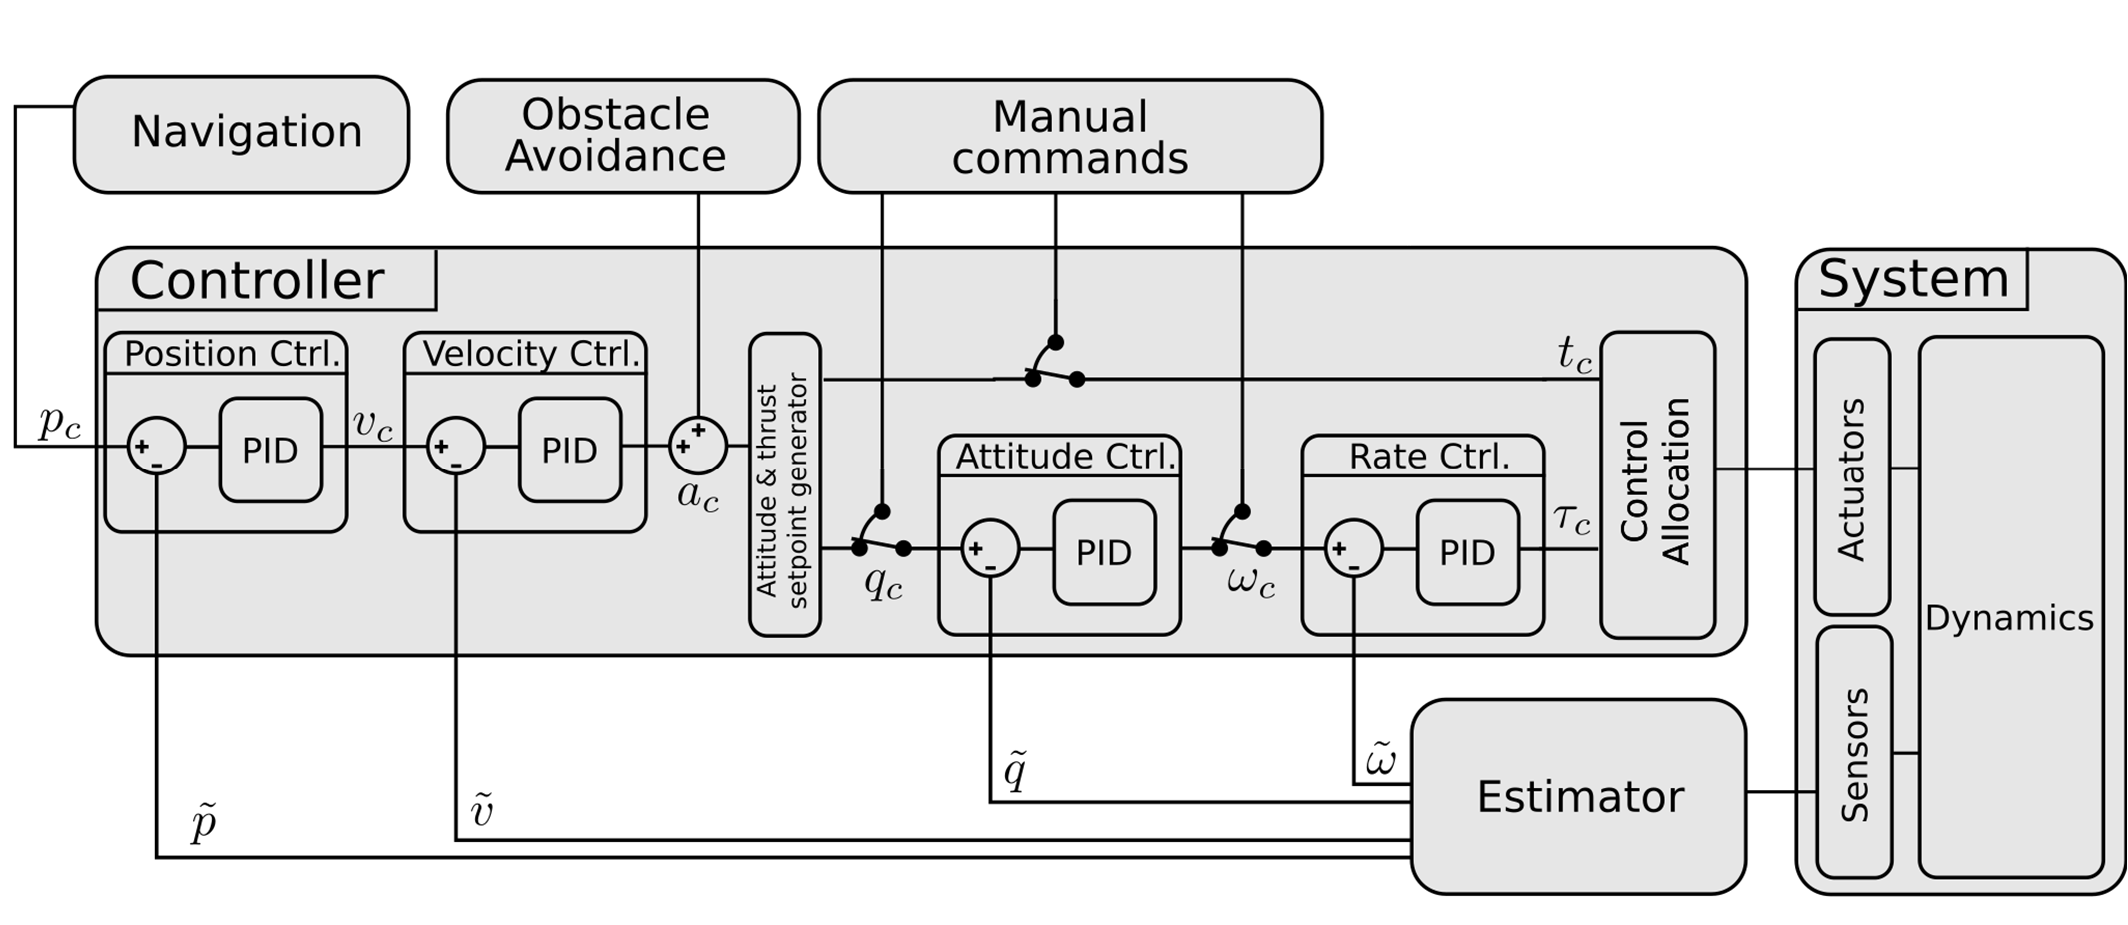
\includegraphics{F:/\#\#\#Learning@EPFL/\#MasterSemester_21Spring/Notes4Review_21Spring/pics/aerial/week2_cascaded_control.png}
\caption{week2\_cascaded\_control}
\end{figure}

\begin{itemize}
\item
  features

  \begin{itemize}
  \item
    insert the obstacle avoidance together with velocity setpoint
  \item
    manual commands send thrust and attitude rate commands
  \item
    \textbf{the lowest level of the controller, the higher bandwidth it
    needs}
  \end{itemize}
\item
  Pros

  \begin{itemize}
  \item
    Decouple translational and rotational dynamics
  \item
    Facilitate implementation of the controller

    implement one by one
  \item
    Better failure diagnosis capability

    modular control architecture for debugging them one by one
  \end{itemize}
\item
  Question: why a more advanced controller?

  \begin{itemize}
  \item
    linear assumption vs nonlinear system
  \item
    more advanced system can bring optimal performance
  \end{itemize}
\end{itemize}

\subsection{Control allocation}\label{header-n616}

\begin{quote}
convert \textbf{thrust \& torque} setpoint into \textbf{actuator}
commands

account for different geometries
\end{quote}

\begin{figure}
\centering
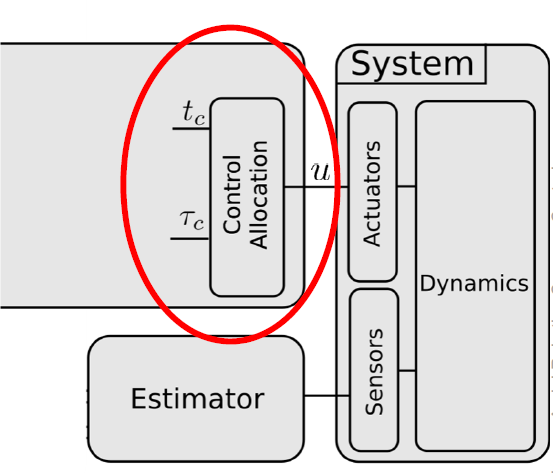
\includegraphics{F:/\#\#\#Learning@EPFL/\#MasterSemester_21Spring/Notes4Review_21Spring/pics/aerial/week2_control_allocation.png}
\caption{week2\_control\_allocation}
\end{figure}

\begin{itemize}
\item
  from \textbf{thrust \& torque} setpoint into \textbf{actuator}

  \(\left[\begin{array}{c}u_{0} \\ \vdots \\ u_{N-1}\end{array}\right]=B\left[\begin{array}{l}\tau_{x} \\ \tau_{y} \\ \tau_{z} \\ t_{z}\end{array}\right]\)
  \(u\) : actuator commands (Nx1)

  \(\mathcal{T}:\) moment setpoints (3x1)

  \(t:\) thrust setpoint \((1 \times 1)\)
\end{itemize}

\subsubsection{Method}\label{header-n627}

\begin{figure}
\centering
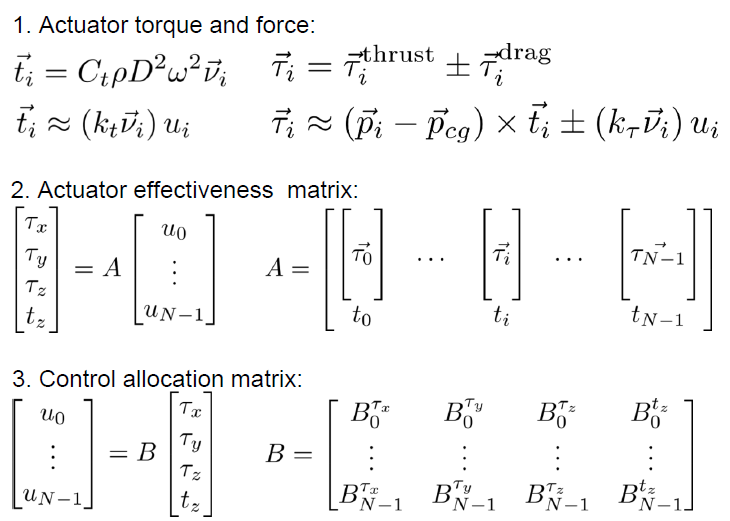
\includegraphics{F:/\#\#\#Learning@EPFL/\#MasterSemester_21Spring/Notes4Review_21Spring/pics/aerial/week2_allocation_method.png}
\caption{week2\_allocation\_method}
\end{figure}

\begin{enumerate}
\def\labelenumi{\arabic{enumi}.}
\item
  Compute generated force and torque of each actuator
\item
  Build matrix "Actuator \textbf{Effectiveness}"
\item
  Compute \textbf{allocation matrix} B as the \textbf{pseudo-inverse} of
  A

  not always square, so using pseudo-inverse (\(B = A^+\))
\end{enumerate}

\subsubsection{Remark}\label{header-n637}

\begin{itemize}
\item
  less effective at producing yaw torque
\item
  yaw torque requires more actuator effort than roll and pitch torque

  \begin{figure}
  \centering
  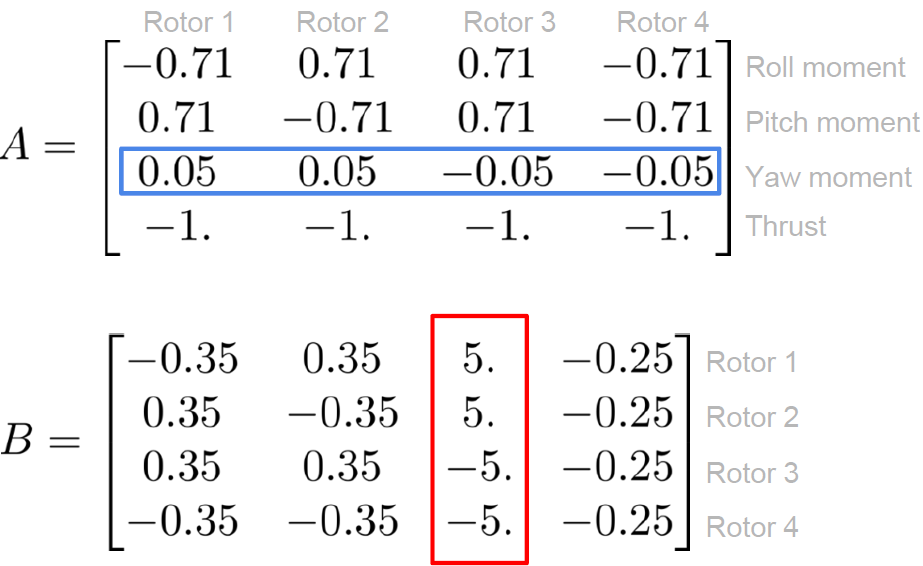
\includegraphics{F:/\#\#\#Learning@EPFL/\#MasterSemester_21Spring/Notes4Review_21Spring/pics/aerial/week2_control_allocation_example.png}
  \caption{week2\_control\_allocation\_example}
  \end{figure}
\end{itemize}

\subsection{Rate control}\label{header-n644}

\textbf{Input} body rate setpoint -\textgreater{} \textbf{Output} torque
to each angle rate

\subsection{Attitude control}\label{header-n646}

\textbf{Input} quaternions setpoint -\textgreater{} \textbf{Output}
torque to each angle rate

\begin{itemize}
\item
  How to compute the quaternion error

  \(\boldsymbol{q}_{e r r}=\boldsymbol{q}_{\boldsymbol{r e f}} \otimes \boldsymbol{q}_{m}^{*}\)
\item
  axis error

  \(\left[\begin{array}{c}
  \Phi_{e} \\
  \Theta_{e} \\
  \Psi_{e}
  \end{array}\right] \approx \operatorname{sgn}\left(q_{e}^{0}\right)\left[\begin{array}{l}
  2 q_{e}^{1} \\
  2 q_{e}^{2} \\
  2 q_{e}^{3}
  \end{array}\right]\)
\end{itemize}

\subsubsection{Full quaternion based attitude control for a
quadrotor}\label{header-n655}

\begin{quote}
Fresk, E. and Nikolakopoulos, G., 2013, July. Full quaternion based
attitude control for a quadrotor. In 2013 European control conference
(ECC) (pp. 3864- 3869). IEEE.
\end{quote}

\begin{itemize}
\item
  without any transformations and calculations in the Euler's angle
  space
\item
  quaternions

  \begin{itemize}
  \item
    scalar + vector part

    \(\boldsymbol{q}=q_{0}+q_{1} \boldsymbol{i}+q_{2} \boldsymbol{j}+q_{3} \boldsymbol{k} = [q_0, q_1, q_2, q_3]^{\mathsf{T}}\)
  \item
    Multiplication of two quaternions p, q is being performed by the
    \textbf{Kronecker product}
  \item
    \(p \otimes q\) represents the combined rotation
  \item
    quaternion multiplication is non-commutative 不遵循交换律
  \item
    All quaternions are assumed to be of \textbf{unitary length}
    单位长度
  \item
    The \textbf{complex conjugate} of a quaternion has the same
    definition as normal complex numbers 复共轭

    \(\operatorname{Conj}(\boldsymbol{q})=\boldsymbol{q}^{*}=\left[\begin{array}{llll}q_{0} & -q_{1} & -q_{2} & -q_{3}\end{array}\right]^{T}\)
  \item
    if the length of the quaternion is unitary then the \textbf{inverse
    is the same as its conjugate} 逆即是复共轭

    \(\operatorname{Inv}(\boldsymbol{q})=\boldsymbol{q}^{-1}=\frac{\boldsymbol{q}^{*}}{\|\boldsymbol{q}\|^{2}} = {q}^{*}\)
  \end{itemize}
\item
  \textbf{Rotation transformation} is built by two quaternion
  multiplications-the normal and its conjugate

  \begin{itemize}
  \item
    rotates the \textbf{vector v from the fixed frame} to the body frame
    represented by q

    \(\boldsymbol{w}=\boldsymbol{q} \otimes\left[\begin{array}{l}0 \\ \mathbf{v}\end{array}\right] \otimes \boldsymbol{q}^{*}\)

    where \(\textbf{v}\) can be rewritten as location in x, y and z
    axis. For example,

    \(R_{x}(\boldsymbol{q})=\boldsymbol{q} \otimes\left[\begin{array}{l}0 \\ 1 \\ 0 \\ 0\end{array}\right] \otimes \boldsymbol{q}^{*}=\left[\begin{array}{c}q_{0}^{2}+q_{1}^{2}-q_{2}^{2}-q_{3}^{2} \\ 2\left(q_{1} q_{2}+q_{0} q_{3}\right) \\ 2\left(q_{1} q_{3}-q_{0} q_{2}\right)\end{array}\right]\)
  \item
    \(u\) is the rotation axis (unit vector) and \(\alpha\) is the angle
    of rotation

    \(\boldsymbol{q}=\cos \left(\frac{\alpha}{2}\right)+\boldsymbol{u} \sin \left(\frac{\alpha}{2}\right)\)
  \end{itemize}
\item
  Calculating quaternions error dynamics

  \begin{itemize}
  \item
    desired \(\mathbf{q}_{ref}\), measured \(\mathbf{q}_{m}\), error
    \(\mathbf{q}_{err}\)-\/-multiplying the reference with the conjugate
    of the estimated quaternion in Kronecker

    \(\boldsymbol{q}_{e r r}=\boldsymbol{q}_{\boldsymbol{r e f}} \otimes \boldsymbol{q}_{m}^{*}\)
  \end{itemize}
\item
  Angular errors: the reference is \textbf{demanding a rotation more
  than π radians}, the closest rotation is the \textbf{inverted
  direction} and this is found by examining q0. If q0 \textless{} 0 then
  the desired orientation is more than π radians away

  \(\left[\begin{array}{c}
  \Phi_{e} \\
  \Theta_{e} \\
  \Psi_{e}
  \end{array}\right] \approx \operatorname{sgn}\left(q_{e}^{0}\right)\left[\begin{array}{l}
  2 q_{e}^{1} \\
  2 q_{e}^{2} \\
  2 q_{e}^{3}
  \end{array}\right]\)

  其中sgn函数就对应着计算\(q_0\)的正负
\end{itemize}

\subsection{Control strategies for multicopters}\label{header-n702}

\begin{itemize}
\item
  \textbf{Inner} loops for attitude dynamics \textbf{stabilization}
\item
  \textbf{Outer} loops for \textbf{translational dynamics}
\end{itemize}

\subsubsection{Linear}\label{header-n708}

\paragraph{Examples}\label{header-n709}

\begin{itemize}
\item
  Proportional Integral Derivative (PID)
\item
  Linear Quadratic Regulator (LQR)
\item
  LQG
\end{itemize}

\paragraph{Features}\label{header-n717}

\begin{itemize}
\item
  a linear \textbf{approximation} of the system dynamics
\item
  used when the attitude of the multicopter involves \textbf{angles that
  are close to zero}
\end{itemize}

\paragraph{PID controller}\label{header-n723}

\begin{itemize}
\item
  Pros: Easy to design; Intuitive to tune manually (not necessarily easy
  on a real drone)
\item
  Cons: Imprecise nature of the model due to inaccurate modelling;
  Limits the performance
\item
  Effects of increasing a parameter independently

  \begin{figure}
  \centering
  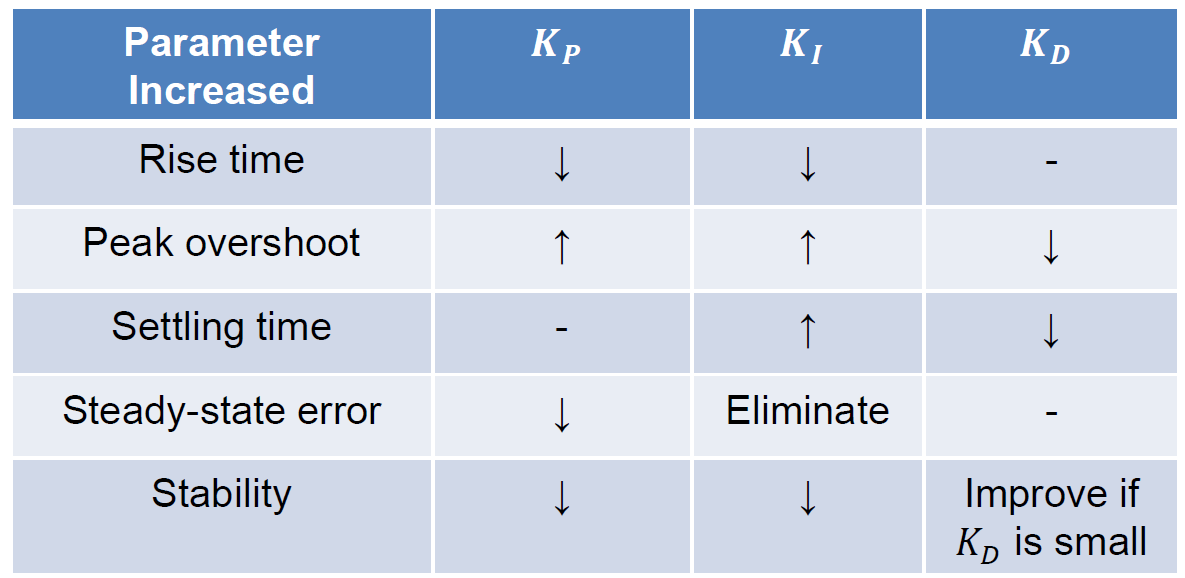
\includegraphics{F:/\#\#\#Learning@EPFL/\#MasterSemester_21Spring/Notes4Review_21Spring/pics/aerial/week3_pid_effect.png}
  \caption{week3\_pid\_effect}
  \end{figure}
\end{itemize}

\paragraph{LQR/LQG}\label{header-n732}

\begin{itemize}
\item
  Features

  \begin{itemize}
  \item
    a multirotor (linearized around an equilibrium point) by
    \textbf{minimizing a suitable cost function}
  \item
    Pros: optimal control method and better than PID (LQR); not need
    complete knowledge of the state and can rely on estimator/observer
    (LQG)
  \item
    Cons: requires tuning of Q and R Matrixes
  \end{itemize}
\item
  Practical example-Foldable Drone

  \begin{itemize}
  \item
    Attitude control (providing \textbf{torques}) requires adaptation
    since morphology has an impact on the rotation dynamics
  \item
    \textbf{should update matrix matrix A during flight}
  \end{itemize}
\item
  Effect of Q and R matrixes

  \begin{itemize}
  \item
    design parameters to penalize (1) the \textbf{state} variables and
    (2) the \textbf{control} signals
  \item
    Large value: stabilize the system with less change in S\textbf{tate
    (Q) and Control input (R)}
  \item
    Small value: stabilize the system without ``caring too much'' about
    ...
  \end{itemize}
\end{itemize}

\subsubsection{Nonlinear}\label{header-n759}

\paragraph{Examples}\label{header-n760}

\begin{itemize}
\item
  Model Predictive Control (MPC)
\item
  Artificial Neural Networks
\end{itemize}

\paragraph{Features}\label{header-n766}

\begin{itemize}
\item
  The \textbf{stability domain} of a drone controlled with a nonlinear
  controller can be \textbf{bigger}
\item
  \textbf{a better model} of the drone can lead to better performances
\item
  \textbf{allows to take explicitly into account aerodynamic effects and
  forces} acting on the drones
\end{itemize}

\subsection{An introduction to fully actuated multirotor
UAVs}\label{header-n774}

\begin{itemize}
\item
  conventional ones have coupling between the horizontal translational
  and rotational dynamics
\item
  fully actuated can help decouple translation and rotation; have direct
  control to corresponding DoF

  key: \textbf{allocation matrix changes}

  \begin{itemize}
  \item
    Fixed-tilt

    easier controller; don't need additional motors; lightweight; cannot
    achieve optimal performance
  \item
    Variable-tilt: change tilt of propellers to achieve desired motion

    can achieve optimal configuration in given task but with complex
    mechatronics and control
  \end{itemize}
\end{itemize}

\subsection{☑️ Checkpoints}\label{header-n788}

\begin{itemize}
\item
  What is the size of the control allocation matrix of an hexacopter
  with \textbf{4 controlled degrees of freedom}?

  \begin{itemize}
  \item
    hexacopter 六轴,6motors
  \item
    Effectiveness matrix: 4x6
  \item
    \textbf{Controller allocation}: 6x4

    Output: 6 motors; input B x (3torque + 1thrust)

    最底层的控制,就是输入是torque+thrust,输出是n个电机的转速
  \item
    Effectiveness: transformation relationship to torque and thrust for
    each rotor
  \end{itemize}
\item
  Why do we use the \textbf{pseudo inverse} instead of standard matrix
  inverse to compute the control allocation matrix from the actuator
  effectiveness matrix?

  there existing other layout of multicopters except for quadcopters
  with 4 rotors
\item
  What happens when a rate setpoint {[}0 0 1{]} is applied?

  rotate counterclockwise with 1 rad/s in yaw angle
\item
  What are the input and output of the rate controller?

  Input: angle rate setpoint + estimated angle rate

  Output: generated angle \textbf{torque}
\item
  What happens when an attitude setpoint {[}0 0 pi/2{]} is applied?

  rotate counterclockwise with pi/2 in yaw angle
\item
  What are the input and output of the attitude controller in a cascaded
  architecture?

  Input: desired quaternion setpoint \textbf{+ estimated} quaternion

  Output: generated angle rotation rate
\item
  How to compute attitude error quaternion from the estimated attitude
  quaternion and the attitude setpoint quaternion?

  \begin{enumerate}
  \def\labelenumi{\arabic{enumi}.}
  \item
    compute quaternion error

    \(\boldsymbol{q}_{e r r}=\boldsymbol{q}_{\boldsymbol{r e f}} \otimes \boldsymbol{q}_{m}^{*}\)
  \item
    calculate angular errors

    \( \left[\begin{array}{c} \Phi_{e} \\ \Theta_{e} \\ \Psi_{e} \end{array}\right] \approx \operatorname{sgn}\left(q_{e}^{0}\right)\left[\begin{array}{l} 2 q_{e}^{1} \\ 2 q_{e}^{2} \\ 2 q_{e}^{3} \end{array}\right]\)
  \end{enumerate}
\end{itemize}

\section{State Estimation (week3\&4)}\label{header-n829}

\subsection{Introduction to State Estimation}\label{header-n830}

\begin{itemize}
\item
  \textbf{STATE}: variables used to describe the mathematical state of a
  dynamical system
\item
  \textbf{ESTIMATION}: finding an approximation of state variables even
  if the data is incomplete, uncertain, or unstable
\item
  \textbf{estimate} something which you \textbf{can not see or measure
  directly}
\end{itemize}

\subsubsection{Why State Estimation in Robotics?}\label{header-n838}

\begin{itemize}
\item
  Perfect model \& sensor are not available; \textbf{Errors} exist in
  \textbf{both sensors \& models}

  \begin{itemize}
  \item
    State of the robot (proprioception)
  \item
    State of the environment (exteroception)
  \end{itemize}
\item
  \textbf{State Estimation on Aerial Robots}

  Height; \textbf{Attitude; Angular velocity} (Most important as they
  are the \textbf{primary variables used for the stabilization} of the
  UAV); linear velocity

  \begin{itemize}
  \item
    main sensors

    \begin{itemize}
    \item
      \textbf{Inertial} Measurement Unit (IMU)
    \item
      \textbf{Height} Measurement (Acoustic, infrared, barometric, laser
      based)
    \item
      Others: Global Navigation Satellite System (GNSS, outdoor) or
      VICON (indoor); Camera, Kinect, LIDAR
    \end{itemize}
  \end{itemize}
\end{itemize}

\subsection{Estimation for deterministic systems}\label{header-n860}

\subsubsection{State Observer (or Luenberger
Observer)}\label{header-n861}

\begin{itemize}
\item
  minimize the error between measured and estimated values
\end{itemize}

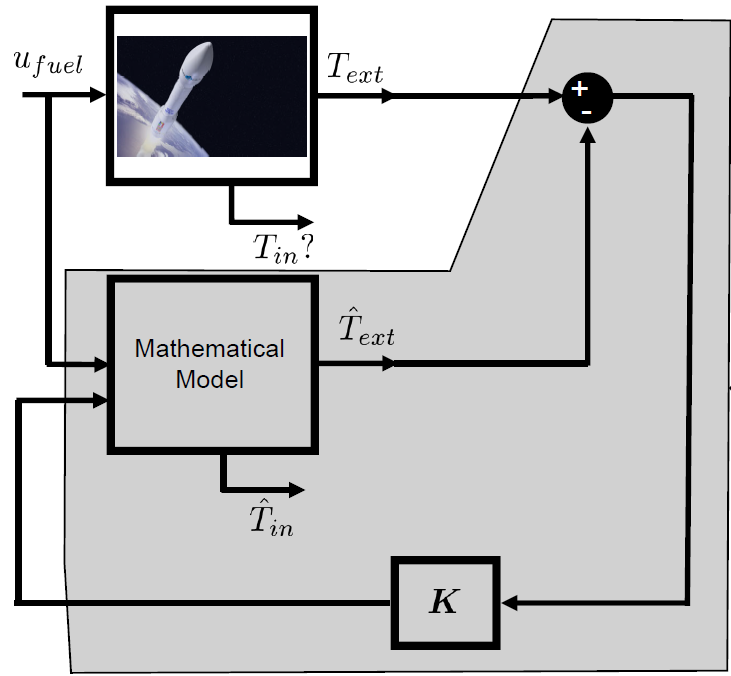
\includegraphics{F:/\#\#\#Learning@EPFL/\#MasterSemester_21Spring/Notes4Review_21Spring/pics/aerial/week3_state_observer.png}
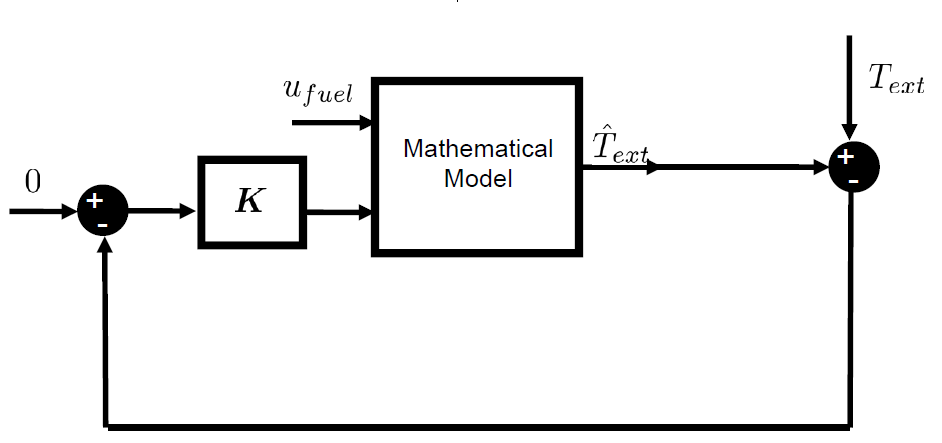
\includegraphics{F:/\#\#\#Learning@EPFL/\#MasterSemester_21Spring/Notes4Review_21Spring/pics/aerial/week3_state_observer2.png}

\begin{itemize}
\item
  how do we choose the ``feedback loop'' gain K ?
\end{itemize}

\subsubsection{Dynamical Systems}\label{header-n869}

\begin{figure}
\centering
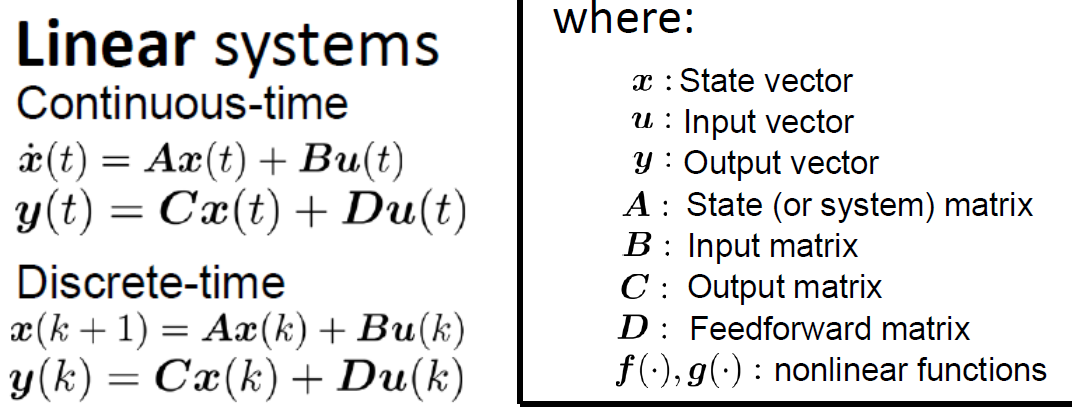
\includegraphics{F:/\#\#\#Learning@EPFL/\#MasterSemester_21Spring/Notes4Review_21Spring/pics/aerial/week3_dynamical_system.png}
\caption{week3\_dynamical\_system}
\end{figure}

\subsubsection{Estimation error}\label{header-n871}

\begin{figure}
\centering
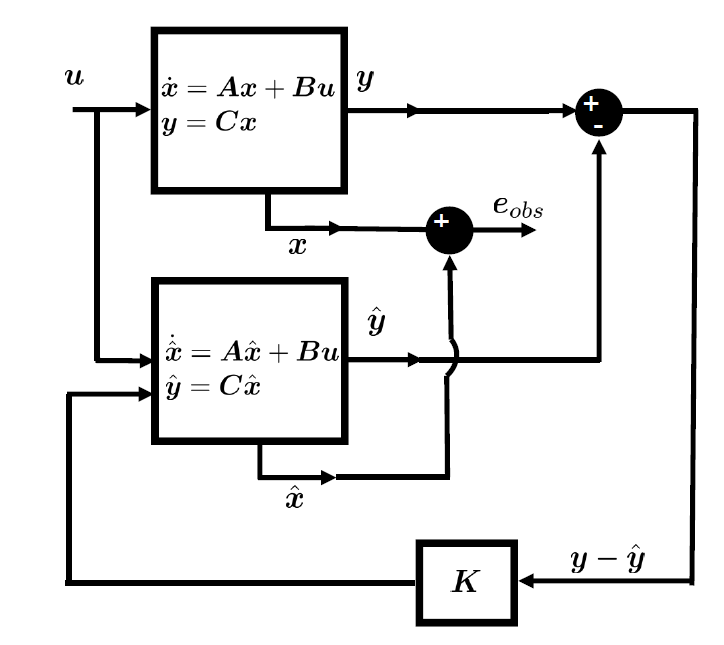
\includegraphics{F:/\#\#\#Learning@EPFL/\#MasterSemester_21Spring/Notes4Review_21Spring/pics/aerial/week4_observer.png}
\caption{week4\_observer}
\end{figure}

\begin{itemize}
\item
  observer error

  \(\dot{e}_{o b s}=(\boldsymbol{A}-\boldsymbol{K} \boldsymbol{C}) \boldsymbol{e}_{o b s} \rightarrow 0\)
  =\textgreater{}
  \(e_{o b s}(t)=e^{(\boldsymbol{A}-\boldsymbol{K} \boldsymbol{C}) t} e_{o b s}\left(t_{0}\right)\)

  \begin{itemize}
  \item
    with linear model

    \(\dot{x} = Ax + Bu\)

    \(\dot{\hat{x}} = A\hat{x} + Bu + K (y-\hat{y})\)

    \(e_{obs} = x - \hat{x}\)
  \end{itemize}
\item
  if A-KC \textless{}0, the error will lead to 0 when t -\textgreater{}
  infinity
\item
  How to choose K?

  \begin{itemize}
  \item
    gives control on the decay rate of the error function
  \item
    similar to P gain in control (if too big, estimation will oscillate)
  \end{itemize}
\end{itemize}

\subsection{State Estimation for stochastic systems}\label{header-n892}

\subsubsection{Recap of fundamental concepts}\label{header-n893}

\begin{itemize}
\item
  Mean and variance encode the \textbf{a‐priori knowledge} of the random
  variable

  \begin{itemize}
  \item
    w: Process noise
  \item
    v: Measurement noise
  \end{itemize}

  \(\dot{\boldsymbol{x}}=\boldsymbol{A} \boldsymbol{x}+\boldsymbol{B} \boldsymbol{u}+\boldsymbol{w}\)
  \(\boldsymbol{y}=\boldsymbol{C} \boldsymbol{x}+\boldsymbol{D} \boldsymbol{u}+v\)
\item
  What is the \textbf{a‐priori information} about uncertainty in our
  problems?

  W/V are known but w/v are zero-mean

  \begin{itemize}
  \item
    W: \textbf{covariance matrix} associated to \textbf{process} noise
  \item
    V: c\textbf{ovariance matrix} associated to \textbf{measurement}
    noise
  \end{itemize}
\item
  What is the statistical \textbf{independence} among the values of a
  random variable in time?

  \(E\left[\boldsymbol{w}(k) \boldsymbol{w}^{T}(k+n)\right]=0 \quad \forall n>0\)
  \(E\left[\boldsymbol{v}(k) \boldsymbol{v}^{T}(k+n)\right]=0 \quad \forall n>0\)
  \(+\) \(E[\boldsymbol{w}(k)]=E[\boldsymbol{v}(k)]=0\)

  \textbf{white noise} stochastic processes -\textgreater{} 期望值都是0
\end{itemize}

\subsubsection{Kalman filter (KF)}\label{header-n915}

\begin{itemize}
\item
  example: estimate drone's roll angle

  \begin{itemize}
  \item
    x: Drone's roll angle
  \item
    u: Roll Body rate
  \item
    y: Drone's roll angle (through IMU)
  \item
    \(w \sim N (0, Q)\): process error \textbf{(only in the dynamics not
    in estimator!)}
  \item
    \(v \sim N (0, R)\): measurement error \textbf{(only in the dynamics
    not in estimator!)}
  \end{itemize}

  \begin{figure}
  \centering
  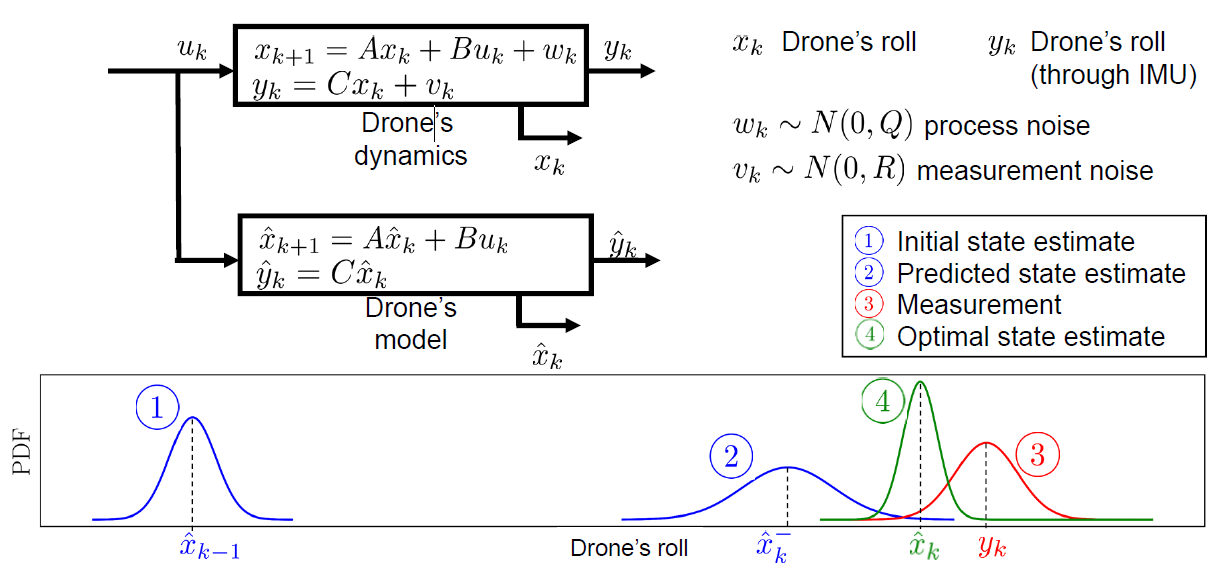
\includegraphics{F:/\#\#\#Learning@EPFL/\#MasterSemester_21Spring/Notes4Review_21Spring/pics/aerial/week5_kf.png}
  \caption{week5\_kf}
  \end{figure}

  \begin{itemize}
  \item
    initial state estimate
  \item
    -\textgreater{} predicted state estimate
  \item
    + measurement
  \item
    =\textgreater{} Optimal state estimate
  \end{itemize}

  \begin{figure}
  \centering
  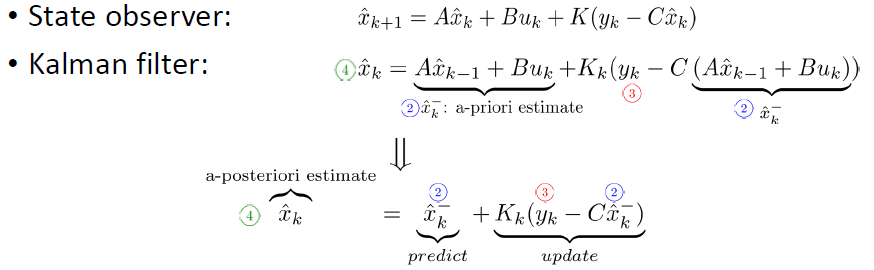
\includegraphics{F:/\#\#\#Learning@EPFL/\#MasterSemester_21Spring/Notes4Review_21Spring/pics/aerial/week4_kf_equ.png}
  \caption{week4\_kf\_equ}
  \end{figure}

  Prediction (A-Priori) + Update
\end{itemize}

use Gaussians to implement a Bayesian filter. That's all the
\textbf{Kalman filter} is - a Bayesian filter that uses Gaussians

\paragraph{PREDICTION}\label{header-n943}

\begin{itemize}
\item
  state \(\hat{x}_{k}^{-}=A \hat{x}_{k-1}+B u_{k}\)
\item
  error covariance \(P_{k}^{-}=A P_{k-1} A^{T}+Q\)

  keep track not only the state but also the covariance (will keep
  increase)
\end{itemize}

\paragraph{UPDATE}\label{header-n950}

\begin{itemize}
\item
  KF Gain \(K_{k}=\dfrac{P_{k}^{-} C^{T}}{C P_{k}^{-} C^{T}+R}\)

  \begin{itemize}
  \item
    trust more in model y\_k

    R-\textgreater{} 0 =\textgreater{} K\emph{k = 1/C =\textgreater{}
    x}k = y\_k/C
  \item
    trust more in measurement x\_k

    P\emph{k -\textgreater{} 0 =\textgreater{}K}k = 0
    =\textgreater{}x\emph{k = x}k\^{}\{\_\}
  \end{itemize}
\item
  Update state
  \(\hat{x}_{k}=\hat{x}_{k}^{-}+K_{k}\left(y_{k}-C \hat{x}_{k}^{-}\right)\)
\item
  \(P_{k}=\left(I-K_{k} C\right) P_{K}^{-}\)

  minimize the Covariance
\end{itemize}

\subsubsection{sensor fusion on a quadrotor}\label{header-n966}

use multiply KF to achieve better estimation

\(\hat{x}_{k_{1 \times 1}}=\hat{x}_{k_{1 \times 1}}^{-}+K_{k_{1 \times n}}\left(y_{k_{n \times 1}}-C_{n \times 1} \hat{x}_{k_{1 \times 1}}^{-}\right)\)

\subsubsection{Intro to EKF, UKF and particle
filters}\label{header-n969}

\paragraph{EKF}\label{header-n970}

\begin{itemize}
\item
  \textbf{linearizes} the nonlinear function \textbf{around the mean of
  the current state estimate}
\end{itemize}

\subparagraph{Overview}\label{header-n974}

\begin{figure}
\centering
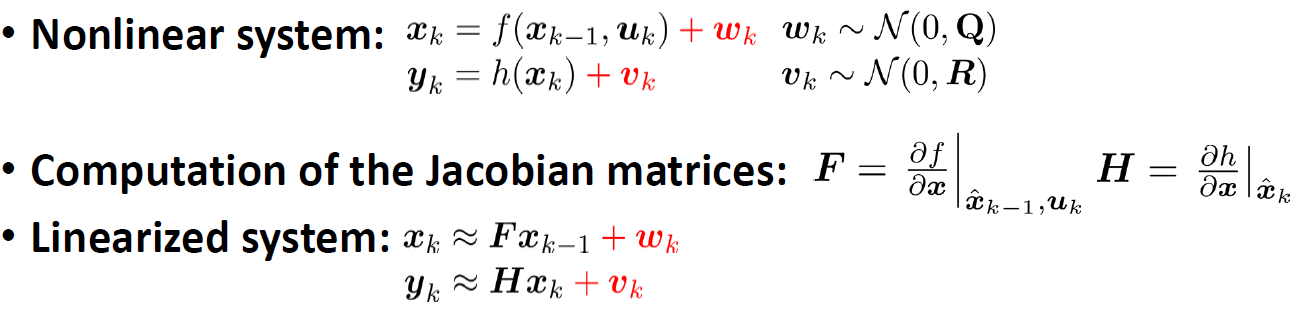
\includegraphics{F:/\#\#\#Learning@EPFL/\#MasterSemester_21Spring/Notes4Review_21Spring/pics/aerial/week4_ekf_equ.png}
\caption{week4\_ekf\_equ}
\end{figure}

\begin{itemize}
\item
  applied to nonlinear system
\item
  linearize around the state estimate value by computing Jacobian
  matrices
\end{itemize}

\subparagraph{Equations}\label{header-n981}

\begin{itemize}
\item
  Predication

  \(\hat{\boldsymbol{x}}_{k}^{-}=f\left(\hat{\boldsymbol{x}}_{k-1}^{-}, \boldsymbol{u}_{k}\right)\)

  \(P_{k}^{-}=F P_{k-1} F^{T}+Q\)

  F-Computed Jacobian matrix

  \(\boldsymbol{F}=\left.\frac{\partial f}{\partial \boldsymbol{x}}\right|_{\hat{\boldsymbol{x}}_{k-1}, \boldsymbol{u}_{k}}\)
\item
  Update

  Near optimal Kalman Filter gain

  \(K_{k}=\dfrac{P_{k}^{-} H^{T}}{H P_{k}^{-} H^{T}+R_k}\)
\end{itemize}

\paragraph{UKF}\label{header-n993}

\begin{itemize}
\item
  take several points to compute/approximate probability distribution
\item
  choose sigma points according to algorithms
\end{itemize}

\paragraph{Particle filters}\label{header-n999}

\begin{itemize}
\item
  Combines the results to estimate the mean and covariance of the state
\item
  !computationally intensive
\item
  Different UKF

  \begin{itemize}
  \item
    Not limited to a Gaussian distribution
  \item
    points are chosen randomly
  \end{itemize}
\end{itemize}

\begin{figure}
\centering
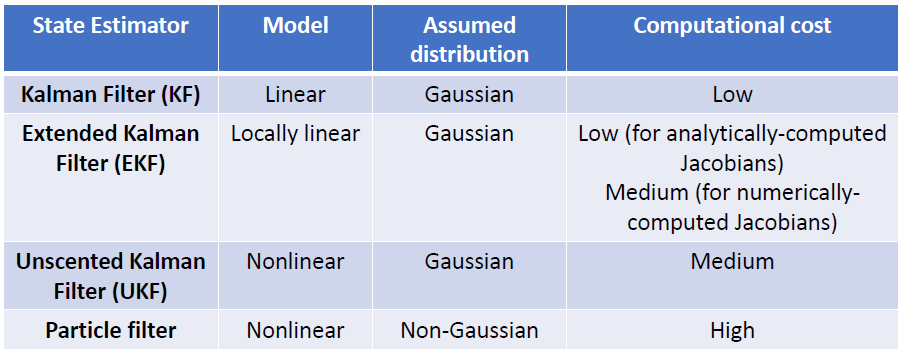
\includegraphics{F:/\#\#\#Learning@EPFL/\#MasterSemester_21Spring/Notes4Review_21Spring/pics/aerial/week5_state_estimation.png}
\caption{week5\_state\_estimation}
\end{figure}

\subsection{State Estimation in aerial robotics}\label{header-n1013}

\subsubsection{in lab settings}\label{header-n1014}

\begin{itemize}
\item
  use MoCap to estimate position and velocity
\end{itemize}

\subsubsection{Outdoor}\label{header-n1018}

\begin{itemize}
\item
  Camera, Depth camera Sensor, ToF Range Sensor to estimate pose and
  height
\end{itemize}

\subsection{☑️ Checkpoints}\label{header-n1022}

\begin{itemize}
\item
  What structure does the Luenberger Observer remind you?

  closed-loop estimation for deterministic systems
\item
  What does the Kalman Filter (KF) gain do?

  determine to trust either more on measurement or a-prior/model
\item
  For which kind of dynamical systems the KF is useful?

  linear continuous system

  !cannot work in discontinuous system
\item
  What do we need to know a-priori if we want to apply the KF?

  state mean \(x_k\) and error covariance \(P_k\)
\item
  What are the advantages/disadvantages of the \textbf{UKF} w.r.t an
  \textbf{EKF}?

  EKF

  \begin{itemize}
  \item
    \textbf{need} linearization
  \item
    Not an optimal estimator (especially nonlinear)
  \item
    may quickly diverge (when incorrect model/wrong covariance init)
  \item
    may difficult to compute Jacobians
  \end{itemize}
\item
  What are the advantages/disadvantages of a \textbf{particle filter}
  w.r.t an \textbf{UKF}?

  PF

  \begin{itemize}
  \item
    Not limited to a Gaussian distribution
  \item
    need more points → more computational time
  \item
    More accurate as long as having enough particles
  \end{itemize}
\end{itemize}

\section{🚧 Navigation (week5)}\label{header-n1059}

\subsection{Velocity control}\label{header-n1060}

\begin{itemize}
\item
  🚧 如果低速飞行,不去调整yaw,不然可能会引起震荡!
\end{itemize}

\subsection{Waypoint Navigation}\label{header-n1064}

\subsection{Dubins Paths}\label{header-n1065}

\subsection{Vector fields}\label{header-n1066}

\subsection{☑️ Checkpoints}\label{header-n1067}

\begin{itemize}
\item
  Which component of the \textbf{acceleration setpoint is converted to
  roll angle?} To \textbf{pitch} angle?

  \begin{itemize}
  \item
    roll 
  \item
    pitch
  \end{itemize}
\item
  Why is navigation based on fixed position setpoint inappropriate for
  fixed-wing drones?

  \begin{itemize}
  \item
    cannot do sharp turning
  \end{itemize}
\item
  What type of segment compose a Dubins path?

  \begin{itemize}
  \item
    arcs of a minimal radius
  \item
    straight lines
  \end{itemize}
\item
  In which case can we construct a RLR Dubins path?

  distance of waypoints is less than the minimal diameter 
\item
  What happens when \textbf{centrifugal acceleration} is not taken into
  account in the formulation of a circle following vector field?

  It will not follow the vectors and cross the circle lines
\end{itemize}

\section{🚧 VIO \& SLAM (week5)}\label{header-n1094}

\subsection{VIO}\label{header-n1095}

\subsection{SLAM}\label{header-n1096}

\subsection{☑️ Checkpoints}\label{header-n1097}

\begin{itemize}
\item
  What is VIO/SLAM useful for?

  \begin{itemize}
  \item
    VIO: Visual inertial odometry

    process of estimating the drone state (position, orientation, and
    velocity) by using only the inputs from Camera(s) and IMU(s)
  \item
    SLAM: Simultaneous Localization and Mapping
  \end{itemize}
\item
  What are the sensors that can be used to do VIO/SLAM?

  Camera(s) and IMU(s)
\item
  What is loop closure?

  the \textbf{recognition} of when the robot has returned to a
  \textbf{previously mapped region} and the use of this information to
  \textbf{reduce the uncertainty in the map estimate.}
\item
  What are the main three VIO paradigms?

  \begin{itemize}
  \item
    Filters

    \begin{itemize}
    \item
      Restrict inference process to \textbf{latest state of the system}
    \end{itemize}
  \item
    Fixed-lag smoothers

    \begin{itemize}
    \item
      Restrict inference process \textbf{to a given time window}
    \end{itemize}
  \item
    Full smoothers

    \begin{itemize}
    \item
      Estimate the \textbf{entire history of the states}
    \item
      More accurate
    \item
      Real‐time operation can become unfeasible
    \end{itemize}
  \end{itemize}
\item
  Why do we use a camera and an IMU for VIO?

  \begin{itemize}
  \item
    \textbf{Cheap and complementary to each other}
  \item
    Camera: \textbf{Precise} during \textbf{slow motion} and provide
    \textbf{rich information}

    Limited output rate; Not robust to scenes with low texture, high
    speed motions
  \item
    IMU: \textbf{Scene independent} and \textbf{High} output
    \textbf{rate}

    Poor signal-to-noise ratio at low accelerations and angular
    velocities; Estimated motion tends to accumulate drift quickly
  \end{itemize}
\end{itemize}

\section{Fixed-wing drones (week6)}\label{header-n1146}

\subsection{Introduction}\label{header-n1147}

\subsection{Structure}\label{header-n1148}

\subsection{Flight Mechanics}\label{header-n1149}

\subsubsection{Control surface}\label{header-n1150}

\begin{itemize}
\item
  Ailerons

  \begin{itemize}
  \item
    attached to the outboard trailing edge of both wings
  \item
    rotate the aircraft around the longitudinal axis (\textbf{roll})
  \end{itemize}
\item
  elevators

  \begin{itemize}
  \item
    hinged to the trailing edge of the horizontal stabilizer
  \item
    around the horizontal or lateral axis (pitch)
  \end{itemize}
\item
  rudder

  \begin{itemize}
  \item
    hinged to the trailing edge of the vertical stabilizer
  \item
    causes an aircraft to yaw or move about the vertical axis
  \end{itemize}
\end{itemize}

\subsubsection{Stability}\label{header-n1173}

longitudinal -\textgreater{} pitching

lateral -\textgreater{} rolling

directional -\textgreater{} yawing

\subsection{Energetics}\label{header-n1177}

\subsubsection{Induced power}\label{header-n1178}

\begin{itemize}
\item
  \textbf{Induced} drag is the drag on the wing that is due to lift
\end{itemize}

\subsubsection{Profile and parasite power}\label{header-n1182}

\begin{itemize}
\item
  The \textbf{total aerodynamic power} is obtained by multiplying the
  \textbf{drag force} by the \textbf{forward velocity}
\end{itemize}

\begin{figure}
\centering
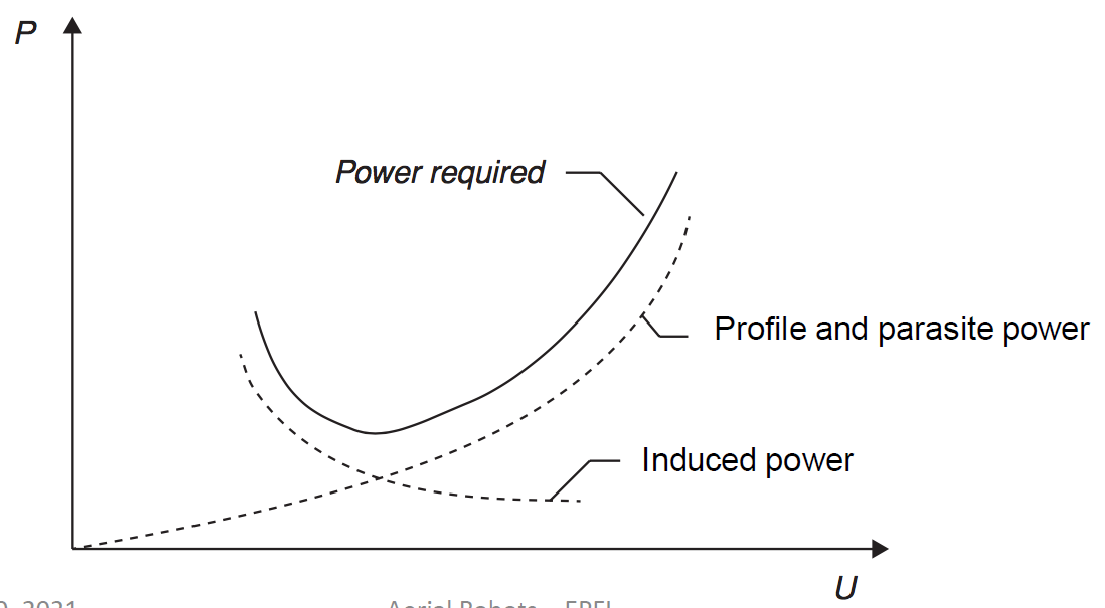
\includegraphics{F:/\#\#\#Learning@EPFL/\#MasterSemester_21Spring/Notes4Review_21Spring/pics/aerial/week6_power_fixed.png}
\caption{week6\_power\_fixed}
\end{figure}

\subsection{☑️ Checkpoints}\label{header-n1187}

\begin{itemize}
\item
  What are the main flight control surfaces in fixed-wing aircrafts?

  \begin{itemize}
  \item
    Ailerons

    \begin{itemize}
    \item
      attached to the outboard trailing edge of both wings
    \item
      rotate the aircraft around the longitudinal axis (\textbf{roll})
    \end{itemize}
  \item
    elevators

    \begin{itemize}
    \item
      hinged to the trailing edge of the horizontal stabilizer
    \item
      around the horizontal or lateral axis (pitch)
    \end{itemize}
  \item
    rudder

    \begin{itemize}
    \item
      hinged to the trailing edge of the vertical stabilizer
    \item
      causes an aircraft to yaw or move about the vertical axis
    \end{itemize}
  \end{itemize}
\item
  What are the \textbf{main stabilization strategies} in fixed-wing
  aircrafts?

  \begin{itemize}
  \item
    Longitudinal stability

    making CoG ahead of the aircraft
  \item
    Lateral stable

    \begin{itemize}
    \item
      Dihedral angle 翅膀上扬
    \item
      Keel effect and Weight distribution
    \end{itemize}
  \item
    Vertical stability-pitch

    making the side surface greater than ahead of the center of gravity
  \end{itemize}
\item
  How is a flying wing/Tailless aircraft controlled and stabilized?

  \begin{itemize}
  \item
    upward reflex (上扬边缘) or elevons (ailerons+elevator) keeps pitch
    in equilibrium
  \end{itemize}
\item
  What are the \textbf{main contributions to power consumption} in
  fixed-wing aircrafts?

  \begin{itemize}
  \item
    Pressure drag + Friction drag
  \item
    \textbf{Induced} drag + Profile drag (wing) + Parasite drag (body)

    \begin{itemize}
    \item
      Induced drag(powers proportional to 1/v)

      drag on the wing that is due to lift
    \item
      Profile drag, Parasite drag (powers proportional to v\^{}3) 
    \end{itemize}
  \end{itemize}
\end{itemize}

\section{Aerial Swarms (week7)}\label{header-n1247}

\subsection{Intro}\label{header-n1248}

\begin{itemize}
\item
  Drone light shows

  \textbf{Centralized} = agents transmit individual position to ground
  computer and receive next location
\item
  Collective Motion in nature

  \textbf{Decentralized} = agents rely on \textbf{local information and
  computation}
\end{itemize}

\subsection{Reynolds flocking algorithm (Reynolds,
1987)}\label{header-n1256}

\begin{itemize}
\item
  radius of communication or neighborhood R
\end{itemize}

\begin{figure}
\centering
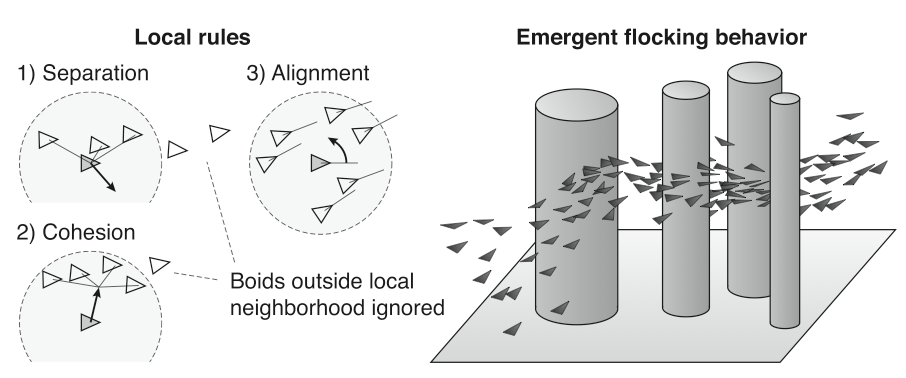
\includegraphics{F:/\#\#\#Learning@EPFL/\#MasterSemester_21Spring/Notes4Review_21Spring/pics/aerial/week7_swarm_reynolds.png}
\caption{week7\_swarm\_reynolds}
\end{figure}

\begin{itemize}
\item
  \textbf{Separation}: avoid collision
\item
  \textbf{Cohesion}: attempt to keep close
\item
  \textbf{Alignment}: attempt to match velocity
\end{itemize}

\subsubsection{Reynolds flocking: model}\label{header-n1268}

\begin{figure}
\centering
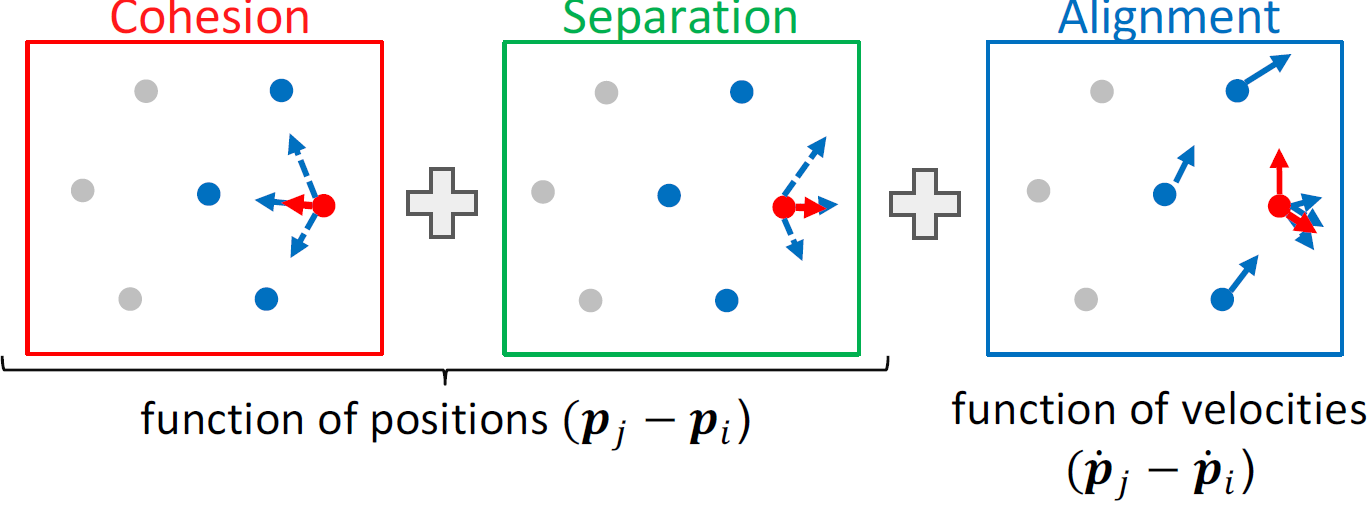
\includegraphics{F:/\#\#\#Learning@EPFL/\#MasterSemester_21Spring/Notes4Review_21Spring/pics/aerial/week7_swarm_reynolds_model.png}
\caption{week7\_swarm\_reynolds\_model}
\end{figure}

\begin{itemize}
\item
  Equations

  \begin{figure}
  \centering
  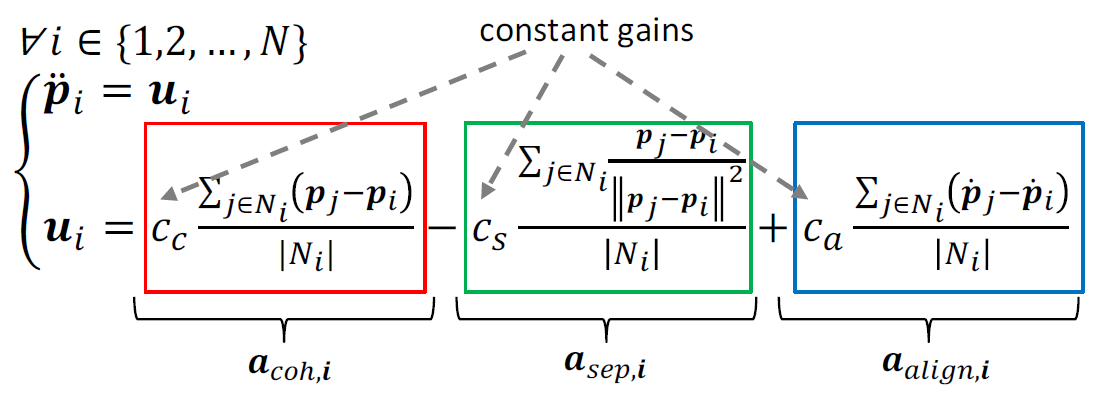
\includegraphics{F:/\#\#\#Learning@EPFL/\#MasterSemester_21Spring/Notes4Review_21Spring/pics/aerial/week7_swarm_reynolds_equ.png}
  \caption{week9\_swarm\_reynolds\_equ}
  \end{figure}

  \begin{itemize}
  \item
    Set of agents in neighborhood \(N\)
  \item
    identity of \(i\)-th agent
  \item
    position \({\mathbf{p}_i}\)
  \item
    velocity \(\dot{\mathbf{p}}_i\)
  \item
    acceleration \(\ddot{\mathbf{p}}_i\) = control command
  \item
    acceleration term due to the cohesion/separation/alignment
    \(\mathbf{a}_{coh,i}\), \(\mathbf{a}_{sep,i}\), and
    \(\mathbf{a}_{align,i}\)
  \item
    constant gains corresponding to the cohesion/separation/alignment
    \(C_c\), \(C_s\), and \(C_a\)
  \end{itemize}
\item
  Equilibrium

  \begin{figure}
  \centering
  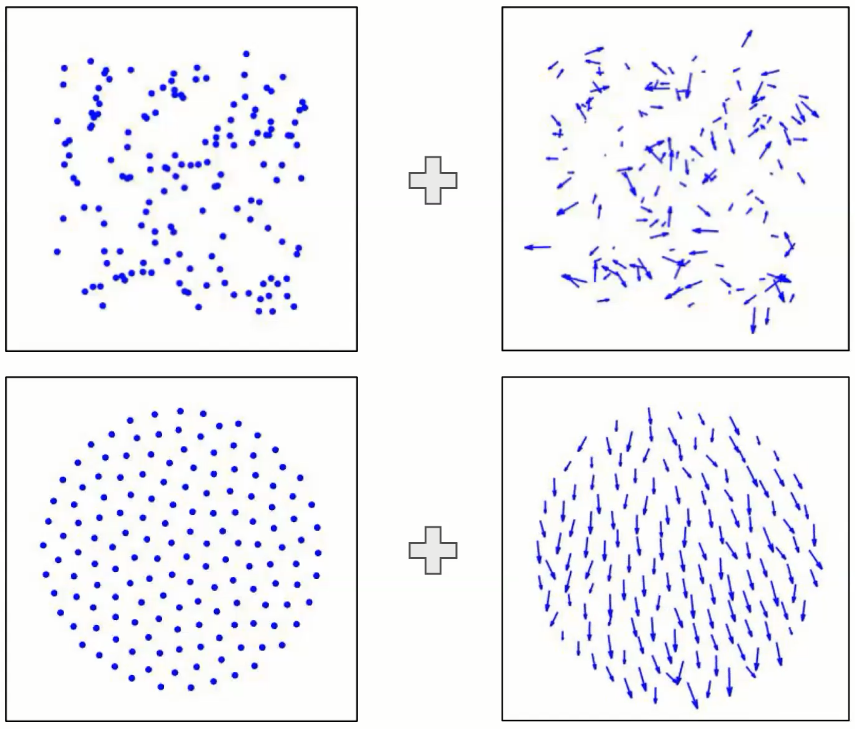
\includegraphics{F:/\#\#\#Learning@EPFL/\#MasterSemester_21Spring/Notes4Review_21Spring/pics/aerial/week7_swarm_reynolds_equilibrium.png}
  \caption{week7\_swarm\_reynolds\_equilibrium}
  \end{figure}

  \begin{itemize}
  \item
    Positions \textbf{converge} to a \underline{lattice formation}
    (晶格式)
  \item
    Velocities \textbf{converge} to the \underline{average of initial
    velocities}

    \(\lim _{t \rightarrow \infty} \dot{\boldsymbol{p}}_{i}=\frac{\sum_{i \in\{1,2, \ldots N\}} \dot{\boldsymbol{p}}_{i}(0)}{N}\)
  \end{itemize}
\end{itemize}

\subsubsection{Reynolds flocking with migration}\label{header-n1298}

\begin{itemize}
\item
  new \textbf{migration rule} steers the swarm towards a desired
  direction

  \begin{itemize}
  \item
    \textbf{replaces} the \textbf{alignment rule}
  \item
    \textbf{cohesion and separation rules are kept} to regulate the
    agents distances
  \end{itemize}

  \begin{figure}
  \centering
  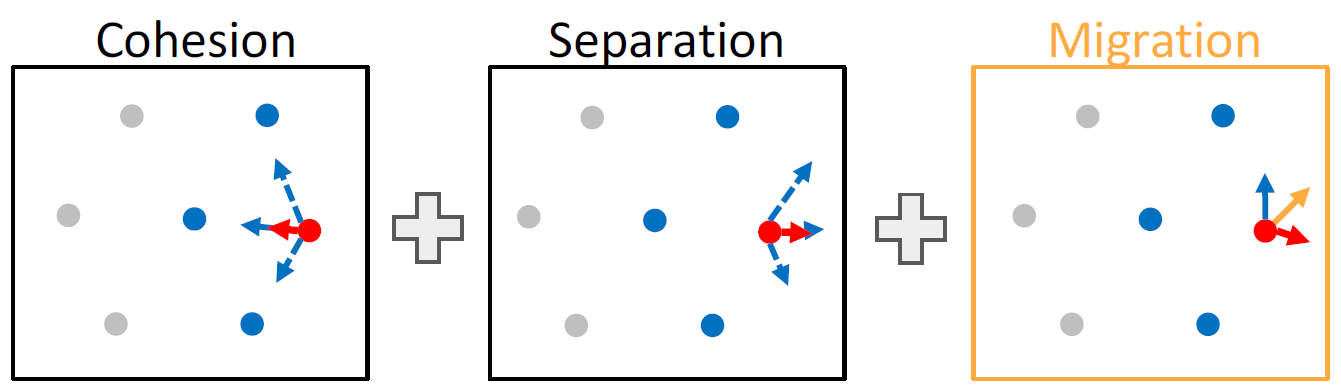
\includegraphics{F:/\#\#\#Learning@EPFL/\#MasterSemester_21Spring/Notes4Review_21Spring/pics/aerial/week7_swarm_reynolds_model_migration.png}
  \caption{week7\_swarm\_reynolds\_model\_migration}
  \end{figure}
\item
  Equation

  \(\ddot{\mathbf{p}}_{i}=\mathbf{u}_{i}\),
  \(\mathbf{u}_{i}=c_{c} \frac{\sum_{j \in N_{i}}\left(\mathbf{p}_{j}-\mathbf{p}_{i}\right)}{\left|N_{i}\right|}-c_{s} \frac{\sum_{j \in N_{i}} \frac{\mathbf{p}_{j}-p_{i}}{\left\|p_{j}-p_{i}\right\|^{2}}}{\left|N_{i}\right|}+c_m \frac{\mathbf{v}_{mig}-\dot{\mathbf{p}}_i}{1}\)

  \(\forall i \in\{1,2, \ldots, N\}\)

  \begin{itemize}
  \item
    parameters

    \begin{itemize}
    \item
      migration velocity \(\mathbf{v}_{mig}\)
    \item
      Denominator = 1 since \textbf{neighbors are not relevant for
      migration}
    \end{itemize}
  \end{itemize}
\end{itemize}

\subsection{Case: Aerial swarms for disaster
mitigation}\label{header-n1320}

\begin{figure}
\centering
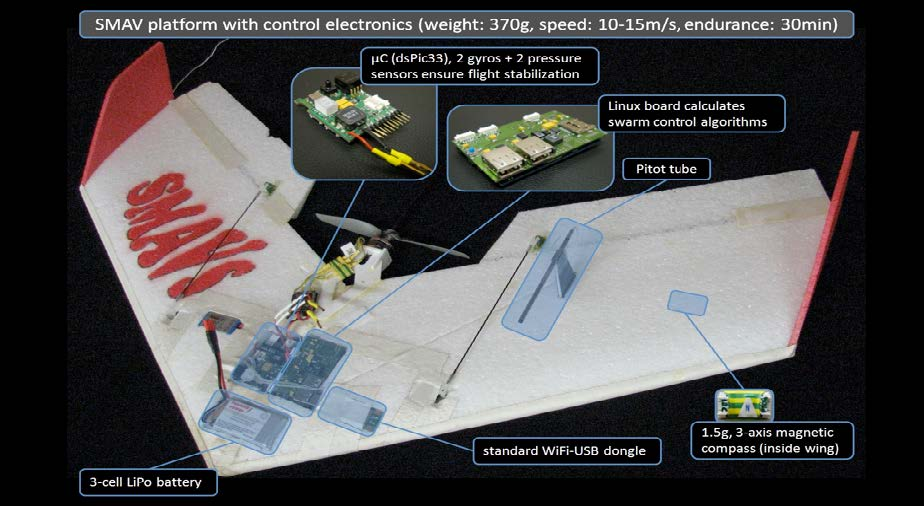
\includegraphics{F:/\#\#\#Learning@EPFL/\#MasterSemester_21Spring/Notes4Review_21Spring/pics/aerial/week7_swarm_project_example.jpg}
\caption{week7\_swarm\_project\_example}
\end{figure}

SMAV platform with control electronics

\subsubsection{Communication radius and turning
angle}\label{header-n1323}

\begin{itemize}
\item
  large communication radius -\textgreater{} can make sharp turn
  together because of knowing the position of other robots
\item
  smaller communication radius -\textgreater{} may separate and gather
  into a flocking often
\end{itemize}

\subsubsection{Virtual agents for flocking with fixed-wing
drones}\label{header-n1329}

\begin{itemize}
\item
  Winged drone flies around Virtual Agent which moves according to
  Reynolds rules

  \begin{figure}
  \centering
  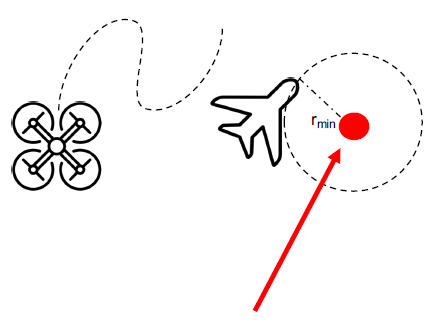
\includegraphics{F:/\#\#\#Learning@EPFL/\#MasterSemester_21Spring/Notes4Review_21Spring/pics/aerial/week7_swarm_virtual.png}
  \caption{week7\_swarm\_virtual}
  \end{figure}
\item
  Varga et al., Distributed Formation Control of Fixed Wing Micro Aerial
  Vehicles for Uniform Area Coverage, IROS 2015

  video: \url{https://youtu.be/FYsd2VckGA0}
\end{itemize}

\subsection{Reynolds flocking with obstacles (Virtual
agents)}\label{header-n1337}

\begin{itemize}
\item
  Obstacles are modelled as \textbf{virtual agents}

  \begin{itemize}
  \item
    Its \textbf{position} is the obstacle's \textbf{closest point} to
    the agent
  \item
    Its \textbf{velocity} is \textbf{perpendicular to the tangent} to
    the obstacle
  \end{itemize}

  \((\mathbf{p}_k, \dot{\mathbf{p}}_k)\) position and velocity of the
  virtual agent
\item
  Virtual agents exert \textbf{separation} and \textbf{alignment}
  effects, but not \textbf{cohesion} (not collide with the agent)
\end{itemize}

\begin{figure}
\centering
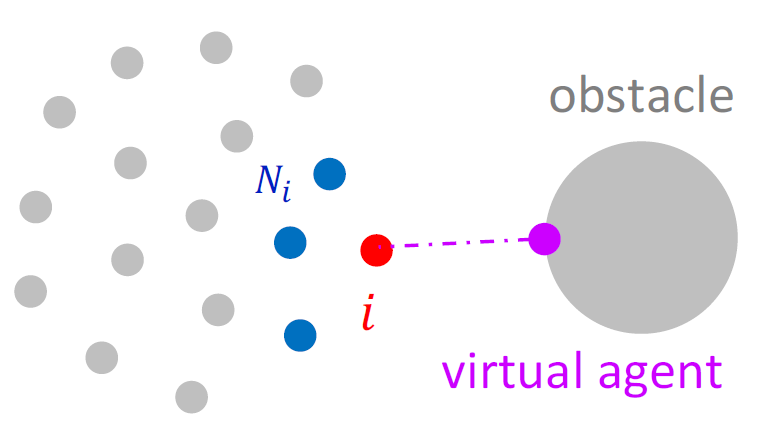
\includegraphics{F:/\#\#\#Learning@EPFL/\#MasterSemester_21Spring/Notes4Review_21Spring/pics/aerial/week7_swarm_reynolds_obs.png}
\caption{week7\_swarm\_reynolds\_obs}
\end{figure}

\begin{itemize}
\item
  Visualization

  \begin{figure}
  \centering
  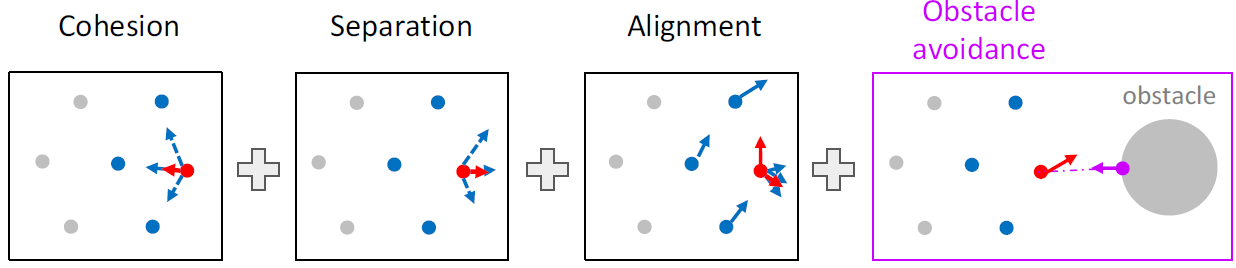
\includegraphics{F:/\#\#\#Learning@EPFL/\#MasterSemester_21Spring/Notes4Review_21Spring/pics/aerial/week7_swarm_reynolds_obs_viz.png}
  \caption{week7\_swarm\_reynolds\_obs\_viz}
  \end{figure}
\item
  Equation (two extra separation and alignment term regarding obstacles)

  \(\ddot{\mathbf{p}}_{i}=\mathbf{u}_{i}\)

  \(\mathbf{u}_{i}=c_{c} \frac{\sum_{j \in N_{i}}\left(\mathbf{p}_{j}-\mathbf{p}_{i}\right)}{\left|N_{i}\right|}-c_{s} \frac{\sum_{j \in N_{i}} \frac{\mathbf{p}_{j}-p_{i}}{\left\|p_{j}-p_{i}\right\|^{2}}}{\left|N_{i}\right|}+c_a \frac{\mathbf{v}_{mig}-\dot{\mathbf{p}}_i}{1} -\left[c_s \frac{\mathbf{p}_k - \mathbf{p}_i}{\Vert \mathbf{p}_k - \mathbf{p}_i \Vert^2} + c_a (\dot{\mathbf{p}}_k - \dot{\mathbf{p}}_i)\right]\)

  \(\forall i \in\{1,2, \ldots, N\}\)
\end{itemize}

\subsection{Other models}\label{header-n1359}

\subsubsection{Vicsek model: particles in confined environments
(密闭环境)}\label{header-n1360}

\begin{quote}
Vasarhelyi et al., Optimized flocking of autonomous drones in confined
environments, Science Robotics, 2019

DOI: \url{http://doi.org/10.1126/scirobotics.aat3536}

Video: https://youtu.be/E4XpyG4eMKE

Project web: http://hal.elte.hu/drones/scirob2018.html
\end{quote}

\begin{itemize}
\item
  Rules

  \begin{itemize}
  \item
    \textbf{Separation}
  \item
    \textbf{Self propulsion}: Makes the agent match a preferred speed
  \item
    \textbf{Friction}: \textbf{Viscosity} (internal friction) for
    alignment and oscillation \textbf{damping}
  \end{itemize}
\item
  Equation

  \(\left\{\begin{array}{l}\dot{\boldsymbol{p}}_{i}=\boldsymbol{u}_{i} \\ \boldsymbol{u}_{i}=\boldsymbol{v}_{s e p, i}+\boldsymbol{v}_{s p p, i}+\boldsymbol{v}_{\text {fric }, i}\end{array}\right.\)
\item
  The full equation contains 12 parameters and \textbf{requires
  heuristic methods for optimization}
\end{itemize}

\subsubsection{Olfati-Saber model}\label{header-n1381}

\begin{quote}
R. Olfati-Saber, Flocking for multi-agent dynamic systems: algorithms
and theory, IEEE Transactions on Automatic Control, 2006
\end{quote}

\begin{figure}
\centering
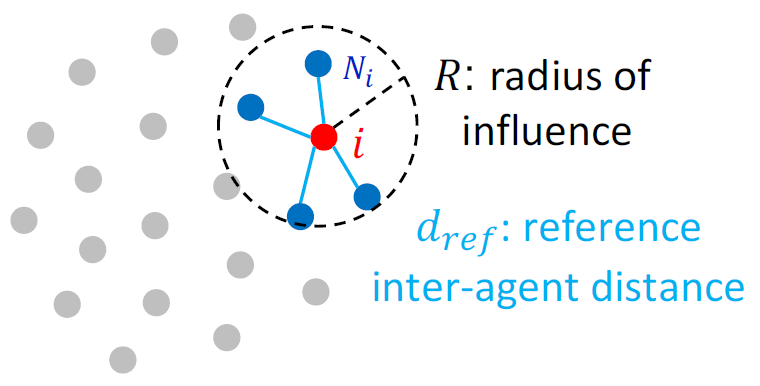
\includegraphics{F:/\#\#\#Learning@EPFL/\#MasterSemester_21Spring/Notes4Review_21Spring/pics/aerial/week7_swarm_olfati_model.png}
\caption{week7\_swarm\_olfati\_model}
\end{figure}

\begin{itemize}
\item
  Rules

  \begin{itemize}
  \item
    Distance matching

    \begin{itemize}
    \item
      Makes the agents \textbf{match a desired inter-agent distance}
    \item
      \textbf{Replaces cohesion and separation} rules of Reynolds model
    \item
      Mathematically defined as a potential function
    \end{itemize}
  \item
    Alignment: attempt to match the velocity and direction
  \end{itemize}

  \begin{figure}
  \centering
  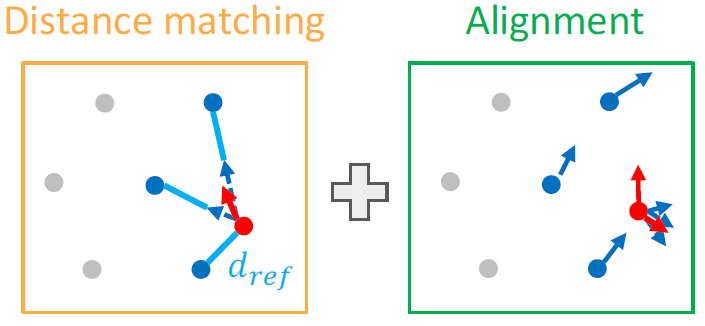
\includegraphics{F:/\#\#\#Learning@EPFL/\#MasterSemester_21Spring/Notes4Review_21Spring/pics/aerial/week7_swarm_olfati_model_viz.png}
  \caption{week7\_swarm\_olfati\_model\_viz}
  \end{figure}
\item
  Equation

  \(\ddot{\mathbf{p}}_{i}=\mathbf{u}_{i}\)

  \(\mathbf{u}_{i}=c_{d} \frac{\sum_{j \in N_{i}} \nabla \left(\rho(\mathbf{p}_{j}-\mathbf{p}_{i}) V (\Vert \mathbf{p}_{j}-\mathbf{p}_{i}\Vert) \right)}{\left|N_{i}\right|}-c_{a} \frac{\sum_{j \in N_{i}} (\dot{\mathbf{p}}_{j}-\dot{\mathbf{p}}_{i})}{\left|N_{i}\right|}\)

  \(\forall i \in\{1,2, \ldots, N\}\)

  \begin{itemize}
  \item
    radius of influence \(R\)
  \item
    desired inter-agent distance \(d_{ref}\)
  \item
    weighting function \(\rho\)
  \item
    distance matching function \(V\)
  \item
    gradient, derivative in three dimensions
    \(\nabla=\left(\frac{\partial}{\partial x}, \frac{\partial}{\partial y}, \frac{\partial}{\partial z}\right)\)
  \end{itemize}
\item
  \textbf{distance matching example}

  \begin{itemize}
  \item
    Components

    \begin{itemize}
    \item
      \textbf{weighting} function 越近影响越大
    \item
      \textbf{distance matching} function 越靠近\(d_{ref}\)越小,线性
    \item
      Result: \textbf{potential function}
    \end{itemize}
  \end{itemize}

  \begin{figure}
  \centering
  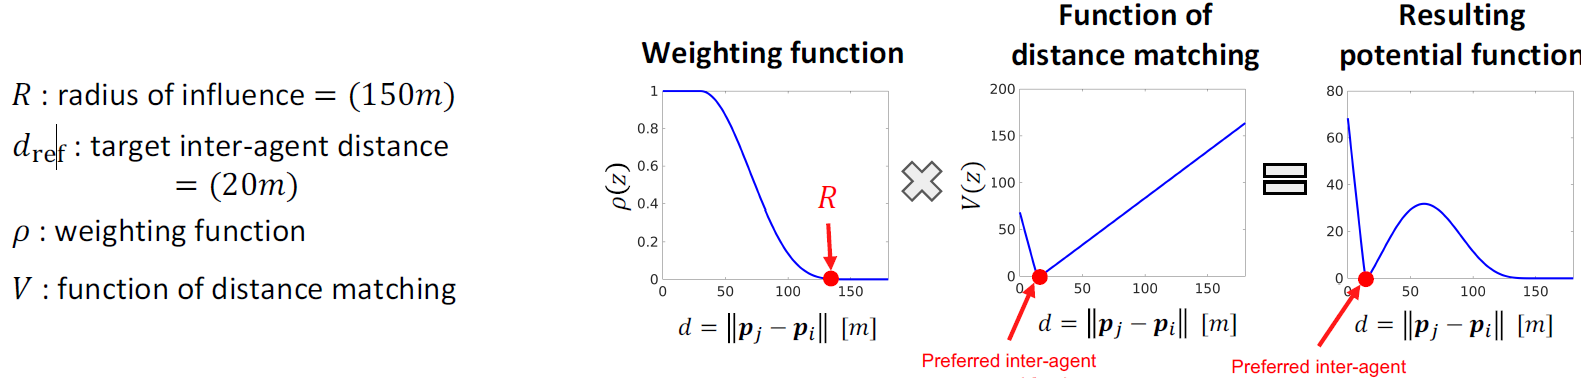
\includegraphics{F:/\#\#\#Learning@EPFL/\#MasterSemester_21Spring/Notes4Review_21Spring/pics/aerial/week7_swarm_olfati_model_dist_mat.png}
  \caption{week7\_swarm\_olfati\_model\_dist\_mat}
  \end{figure}

  \begin{itemize}
  \item
    Note

    \begin{itemize}
    \item
      Principle of minimum potential: \textbf{minimum} defines the
      stable equilibrium of the system
    \item
      \(d_{ref}\) is a stable equilibrium
    \item
      The force acting on an agent is zero in the minimum of the
      potential. For \(d=d_{ref}\), it holds
      \(\nabla(\rho V)=\mathbf{0}\)
    \end{itemize}
  \end{itemize}
\end{itemize}

\subsection{Drone Swarms}\label{header-n1440}

\begin{quote}
Coppola et al., A Survey on Swarming With Micro Air Vehicles:
Fundamental Challenges and Constraints, Front. Robot. AI, `20
\end{quote}

\begin{figure}
\centering
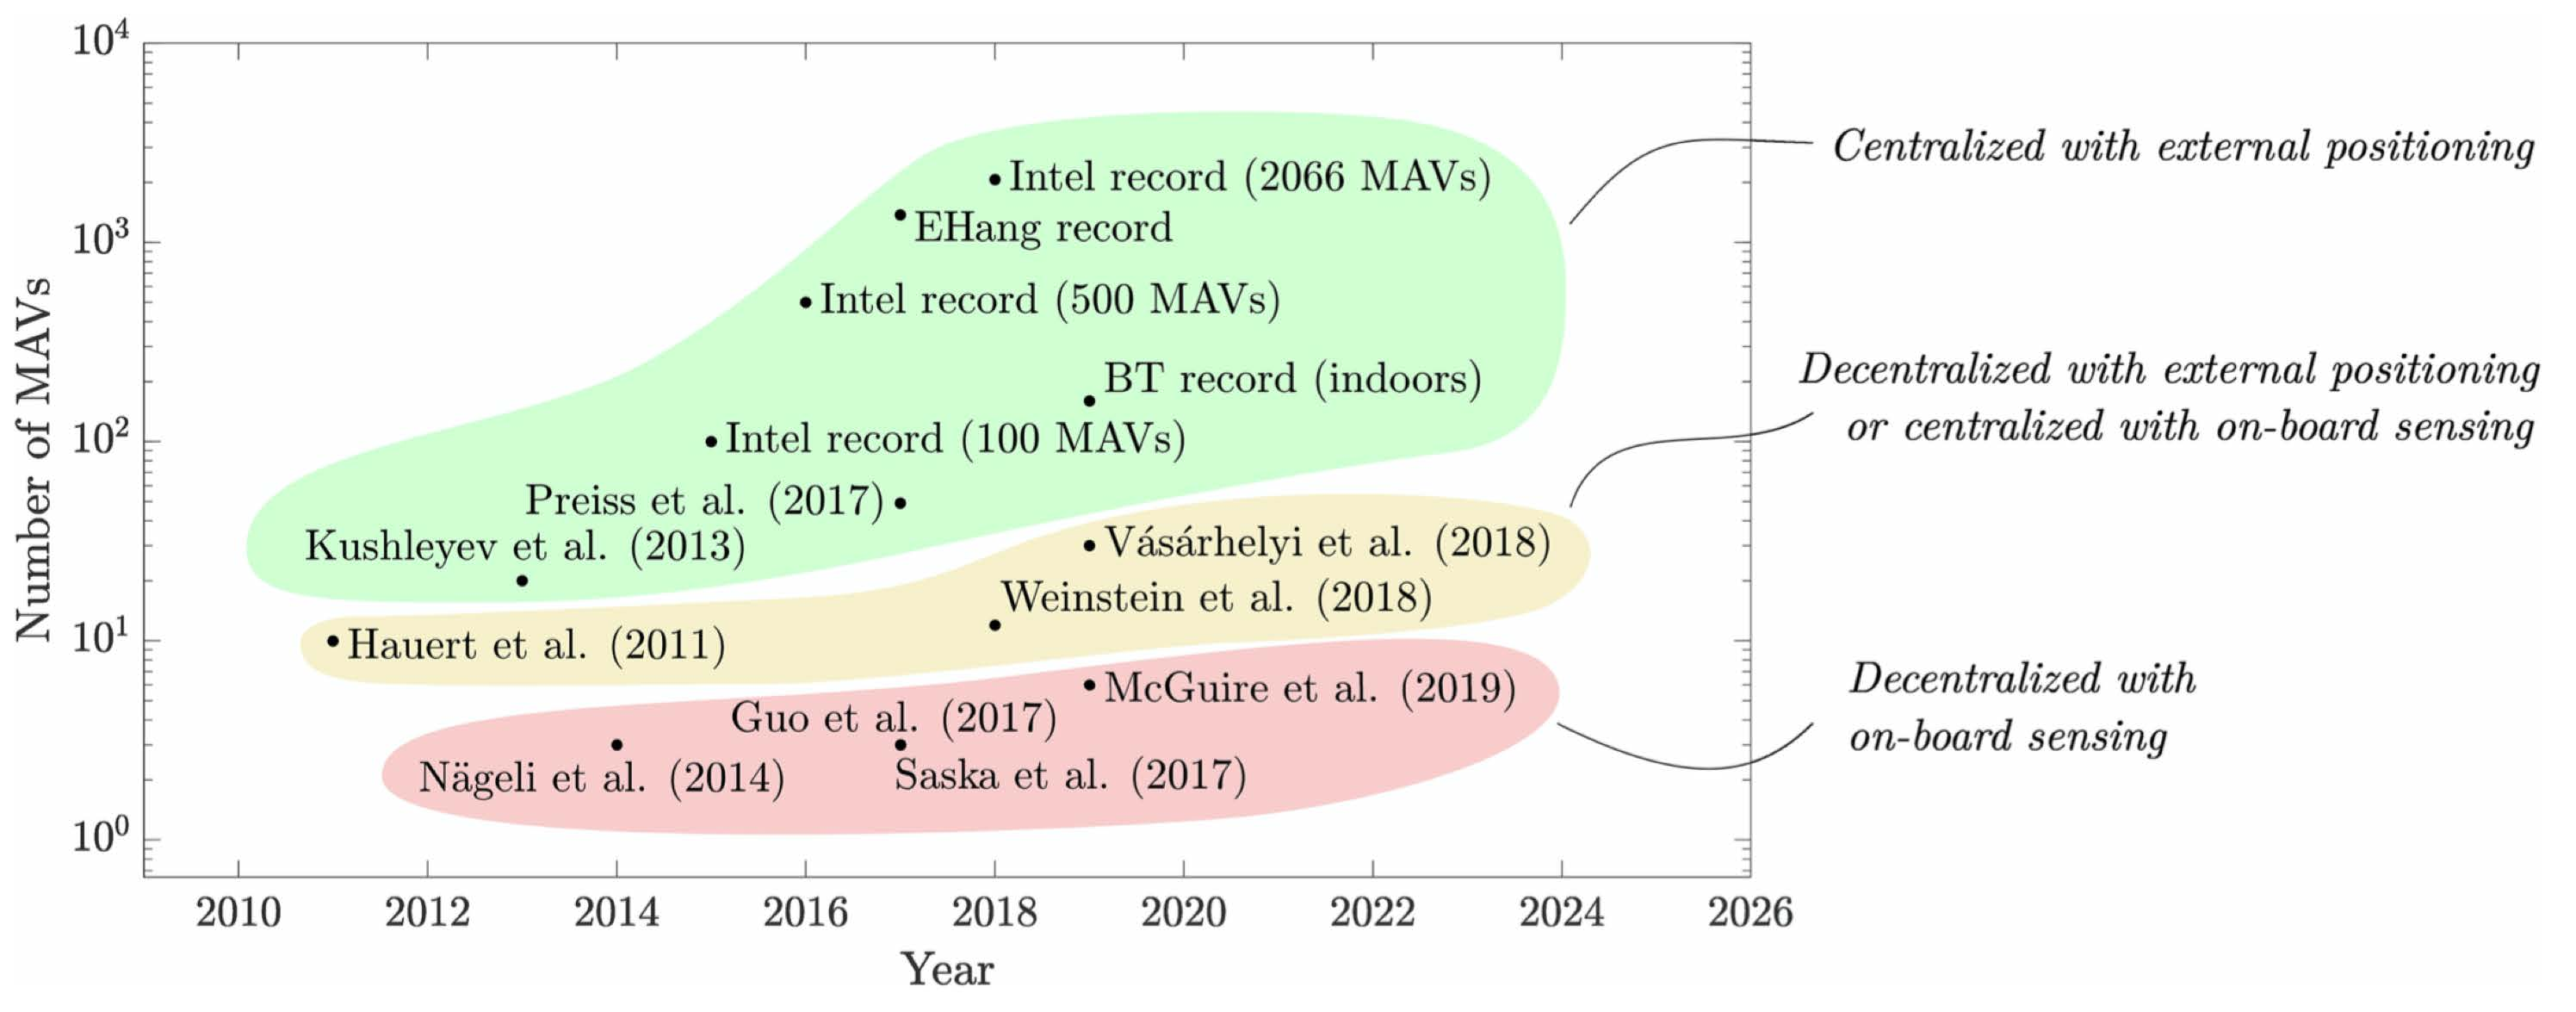
\includegraphics{F:/\#\#\#Learning@EPFL/\#MasterSemester_21Spring/Notes4Review_21Spring/pics/aerial/week7_swarm_survey.jpg}
\caption{week7\_swarm\_survey}
\end{figure}

The combination of centralized planning/control with external
positioning has \textbf{allowed to fly significantly larger swarms}. The
\textbf{numbers are lower} for the \textbf{works featuring decentralized
control with external positioning}, or centralized control with local
sensing

\textbf{Three categories}

\begin{enumerate}
\def\labelenumi{\arabic{enumi}.}
\item
  Centralized with external positioning

  \begin{quote}
  latest: September 20 2020

  3,051 drones

  News:
  https://www.guinnessworldrecords.com/news/2020/10/3051-drones-create-spectacular-record-breaking-light-show-in-china
  (Company: https://www.dmduav.com/)

  YouTube: https://youtu.be/44KvHwRHb3A

  Bilibili: https://www.bilibili.com/video/BV1jt4y1q762
  \end{quote}
\item
  Decentralized with external positioning or centralized with on-board
  sensing

  Vasarhelyi et al. (2019)
\item
  Decentralized with on-board sensing

  Saska et al. (2017)
\end{enumerate}

\subsection{Visual information in flocking}\label{header-n1461}

\subsubsection{Soria2019IRC-influence of limited visual sensing using
Reynolds}\label{header-n1462}

\begin{quote}
Soria et al., The influence of limited visual sensing on the Reynolds
flocking algorithm, 2019
\end{quote}

\begin{itemize}
\item
  generate flocks with different fields of view

  \begin{figure}
  \centering
  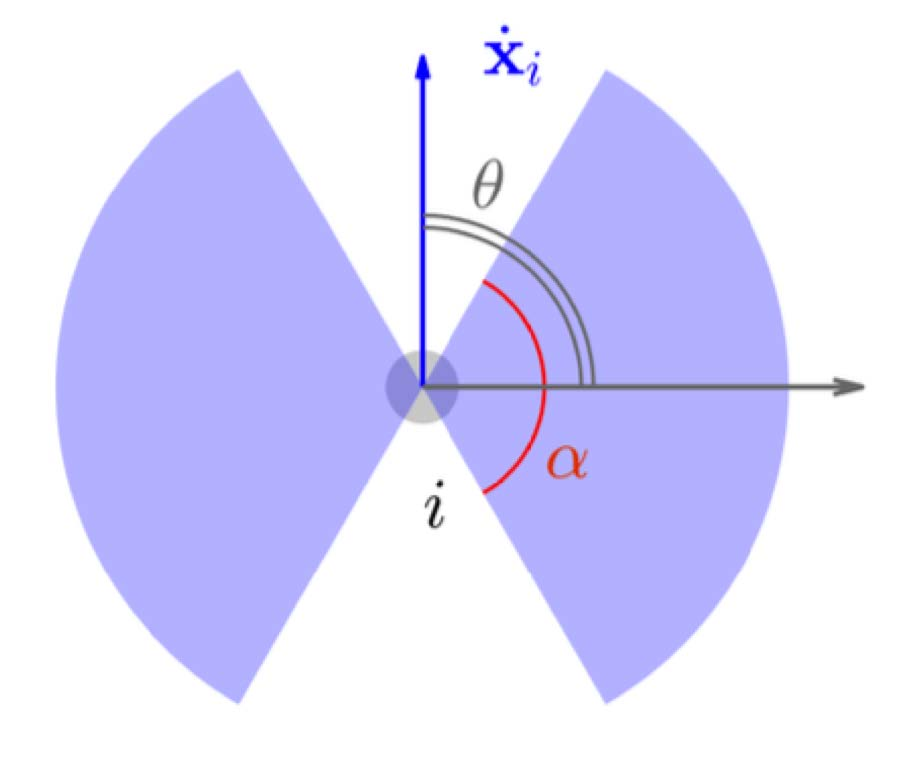
\includegraphics{F:/\#\#\#Learning@EPFL/\#MasterSemester_21Spring/Notes4Review_21Spring/pics/aerial/week7_swarm_limited_vision.jpg}
  \caption{week7\_swarm\_limited\_vision}
  \end{figure}

  \begin{itemize}
  \item
    azimuth/方位角 \(\theta [^{\circ}]\)
  \item
    width \(\alpha [^{\circ}]\)
  \end{itemize}

  \begin{figure}
  \centering
  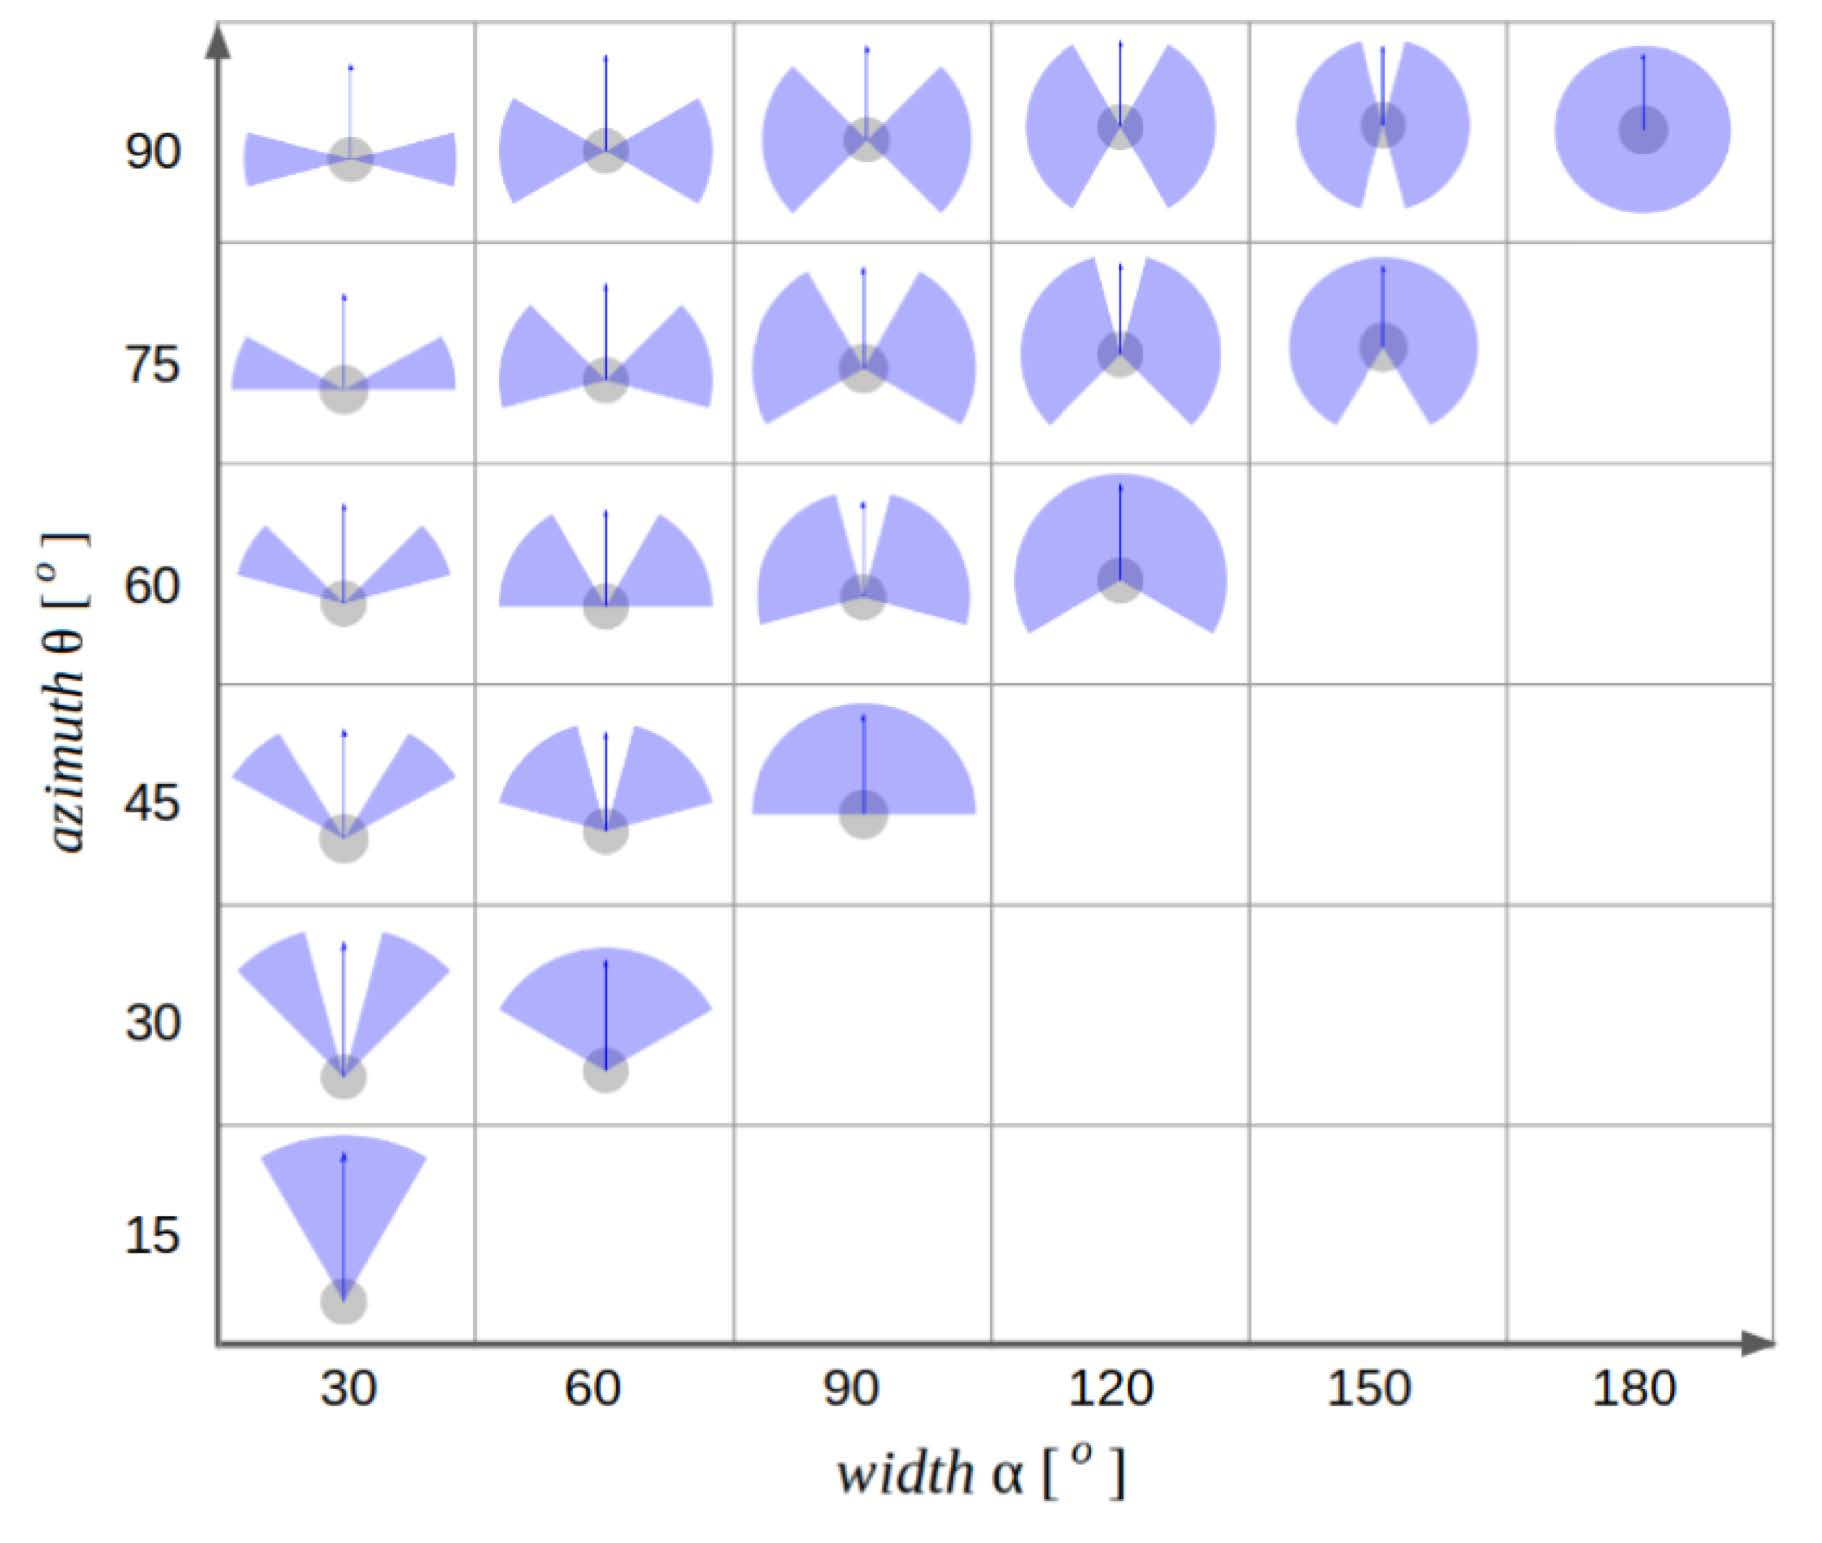
\includegraphics{F:/\#\#\#Learning@EPFL/\#MasterSemester_21Spring/Notes4Review_21Spring/pics/aerial/week7_swarm_limited_vision_tests.jpg}
  \caption{week7\_swarm\_limited\_vision\_tests}
  \end{figure}
\item
  measure flocking performance (all individuals in the flock have the
  same visual configuration)

  \begin{itemize}
  \item
    \textbf{Order}: measure of alignment
  \item
    \textbf{Safety}: ability to avoid collisions
  \item
    \textbf{Union}: ability to stay informed on neighbors
  \item
    \textbf{Connectivity}: ability to broadcast messages among drones
  \end{itemize}

  \begin{figure}
  \centering
  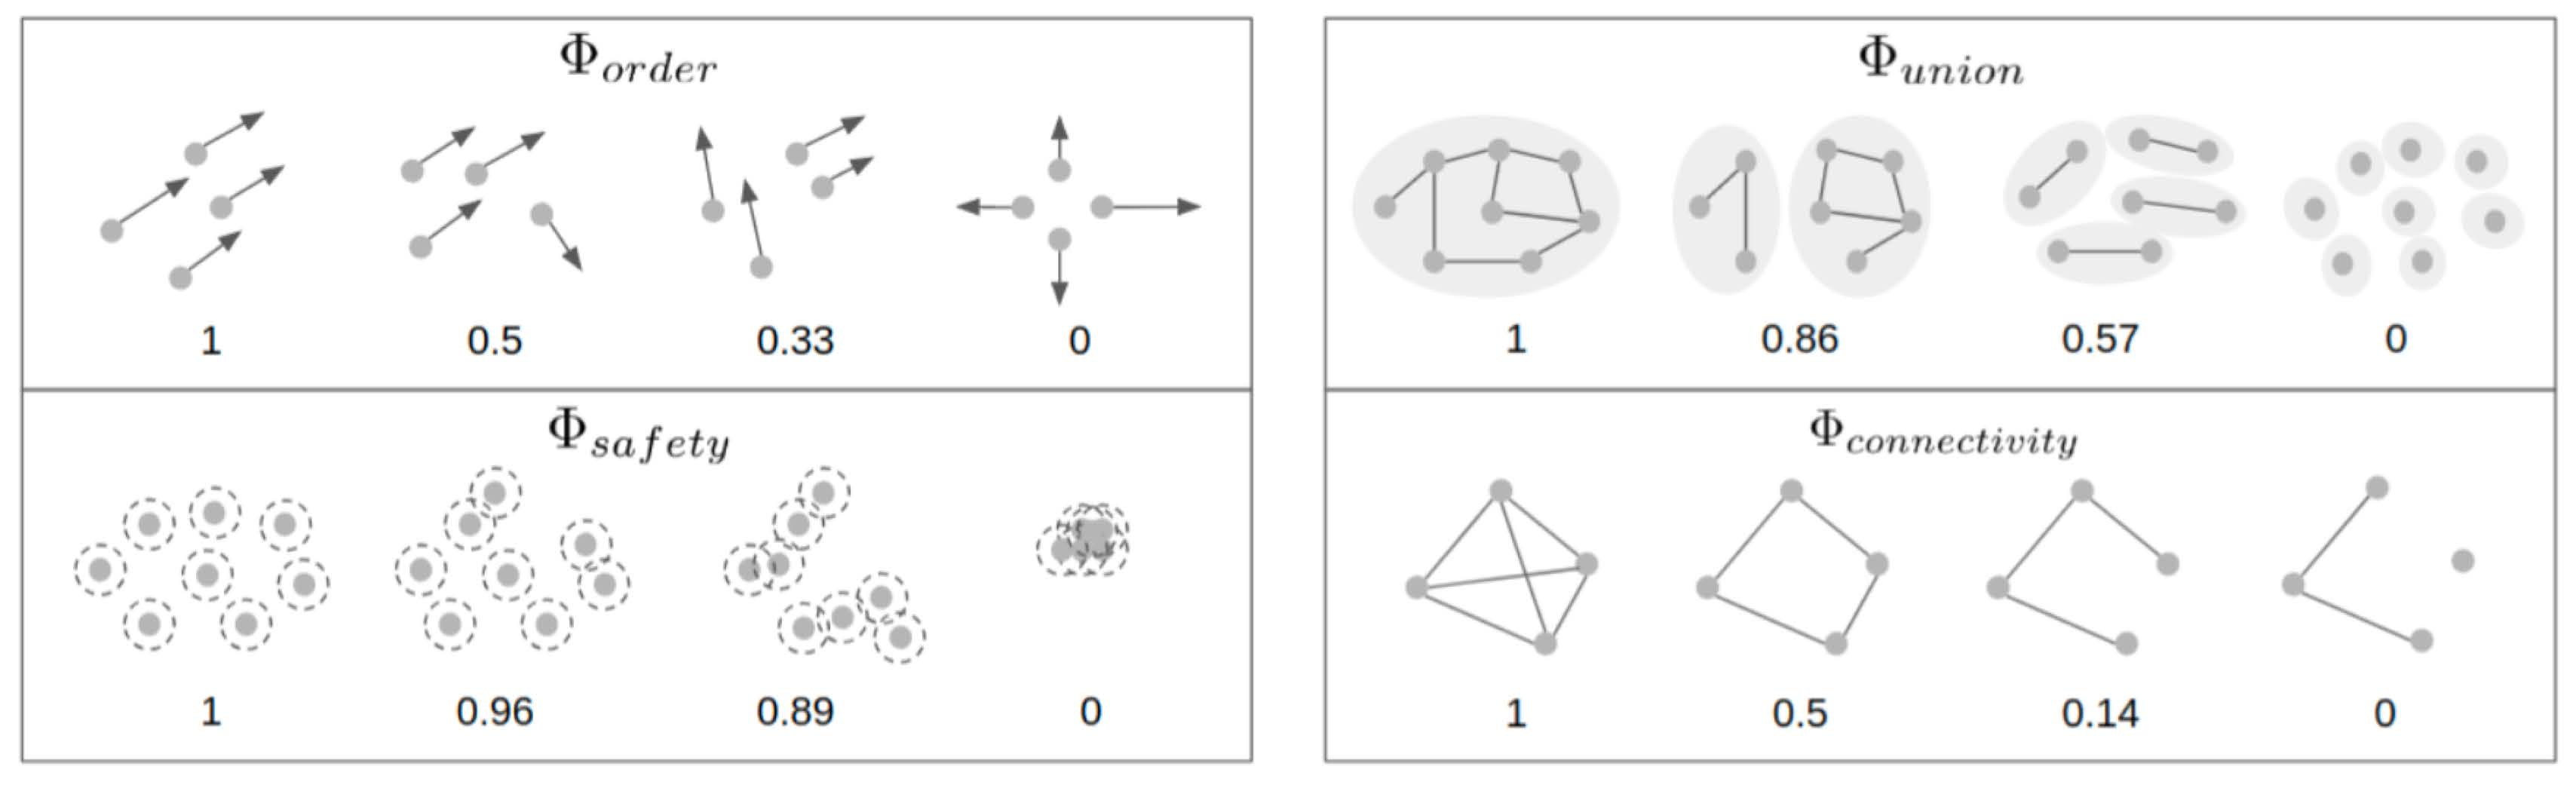
\includegraphics{F:/\#\#\#Learning@EPFL/\#MasterSemester_21Spring/Notes4Review_21Spring/pics/aerial/week7_swarm_limited_vision_metrics.jpg}
  \caption{week7\_swarm\_limited\_vision\_metrics}
  \end{figure}
\item
  results

  \begin{figure}
  \centering
  \includegraphics{F:/\#\#\#Learning@EPFL/\#MasterSemester_21Spring/Notes4Review_21Spring/pics/aerial/week7_swarm_limited_vision_results.png}
  \caption{week7\_swarm\_limited\_vision\_results}
  \end{figure}

  \begin{itemize}
  \item
    focus on order and safety (alignment and collision prevention
    capability)
  \item
    largest azimuth and FoV has best performance
  \item
    increase in either azimuth or FoV only will degrade the performance
  \item
    safety can be achieved even with lower FoV
  \end{itemize}
\end{itemize}

\subsubsection{Schilling2019RAL-Learning to flock in simulation with
vision}\label{header-n1499}

\begin{quote}
Schilling et al., Learning Vision-Based Flight in Drone Swarms by
Imitation, RAL2019
\end{quote}

\begin{itemize}
\item
  use 6 cameras in each side
\item
  training on a dataset to generate the velocity vector for the drone
\end{itemize}

\begin{figure}
\centering
\includegraphics{F:/\#\#\#Learning@EPFL/\#MasterSemester_21Spring/Notes4Review_21Spring/pics/aerial/week7_swarm_vision_Schilling19RAL.png}
\caption{week7\_swarm\_vision\_Schilling19RAL}
\end{figure}

\begin{itemize}
\item
  Stages

  \begin{itemize}
  \item
    Dataset generation: Flocking algorithm as ground truth
  \item
    Training phase: Learn \textbf{mapping between vision and control
    output}
  \item
    Vision-based control: \textbf{Neural controller for collision-free
    and cohesive flight}
  \end{itemize}
\item
  Note

  \begin{itemize}
  \item
    work well in simulation indoor environment
  \item
    it can be robust when individuals has different migration points
  \item
    cannot generalize well in background clutter and different lighting
    condition
  \end{itemize}
\end{itemize}

\subsubsection{Schilling2021RAL-Learning to flock outdoor with
vision}\label{header-n1527}

\begin{quote}
Schilling et al., Vision-Based Drone Flocking in Outdoor Environments,
RAL2021
\end{quote}

\begin{figure}
\centering
\includegraphics{F:/\#\#\#Learning@EPFL/\#MasterSemester_21Spring/Notes4Review_21Spring/pics/aerial/week7_swarm_vision_Schilling2021RAL.png}
\caption{week7\_swarm\_vision\_Schilling2021RAL}
\end{figure}

\begin{itemize}
\item
  Setup

  \begin{itemize}
  \item
    Drone with only with 4 cameras in four side
  \item
    RTK GNSS is used to compute performance
  \item
    train YOLOv3 tiny to recognize other drones using YOLO
  \end{itemize}
\item
  Control method

  \begin{figure}
  \centering
  \includegraphics{F:/\#\#\#Learning@EPFL/\#MasterSemester_21Spring/Notes4Review_21Spring/pics/aerial/week7_swarm_vision_Schilling2021RAL_control.png}
  \caption{week7\_swarm\_vision\_Schilling2021RAL\_control}
  \end{figure}

  \begin{enumerate}
  \def\labelenumi{\arabic{enumi}.}
  \item
    Real-time drone detection

    \begin{itemize}
    \item
      Input: images from 4 cameras
    \item
      Output: x,y coordinates of perceived drones in image frame
      coordinates

      known size to compute corresponding distance
    \end{itemize}
  \item
    Multi-agent state tracking

    \begin{itemize}
    \item
      Input: Locations of drones \& noise models
    \item
      Output: \textbf{Range and bearing} of all perceived drones with
      \textbf{noise}
    \end{itemize}
  \item
    Potential-field-based control

    \begin{itemize}
    \item
      Input: Range and bearing of all perceived drones
    \item
      Output: \textbf{velocity vector} resulting from Reynolds algorithm
    \end{itemize}
  \end{enumerate}
\end{itemize}

\subsection{☑️ Check points}\label{header-n1567}

\begin{itemize}
\item
  What information does each agent receive in the Reynolds flocking
  algorithm?

  position and velocity of self and neighbor agents
\item
  How are obstacles modeled in Reynold's flocking

  virtual agent; integrate into equations with \textbf{alignment and
  separation term} (non cohesion)
\item
  How is a migration point incorporated in flocking algorithms

  add a migration velocity term
\item
  What does the Olfati-Saber algorithm ensure?

  No collision. The \textbf{acting force} will be zero when reach the
  preferred distance \(d_{ref}\)
\item
  What are the three steps of vision-based drone flocking algorithm?

  \begin{enumerate}
  \def\labelenumi{\arabic{enumi}.}
  \item
    Real-time \textbf{drone detection}
  \item
    Multi-agent \textbf{state tracking}
  \item
    Potential-field-based \textbf{control}
  \end{enumerate}

  images from 4 cameras -\textgreater{} x,y coordinates of perceived
  drones in images -\textgreater{} Range and bearing of all perceived
  drones -\textgreater{} velocity vector
\end{itemize}

\section{Flapping-Wing (week8)}\label{header-n1591}

\subsection{Introduction}\label{header-n1592}

\begin{itemize}
\item
  \textbf{lift} and \textbf{thrust} generation, and \textbf{maneuvers}
  mostly obtained by \textbf{using the wings}
\item
  imitate the flapping-wing flight of birds, bats, and insects
\item
  \textbf{scale down better} then rotary crafts and fixed wing UAVs
\item
  \textbf{Challenges}:

  \begin{itemize}
  \item
    Increased mechanical and control complexity
  \item
    Complex modelling due to unsteady aerodynamics
  \end{itemize}
\end{itemize}

\subsection{Structure}\label{header-n1607}

\begin{quote}
categories were determined to be the tail (1) and wing design (2)
\end{quote}

\begin{itemize}
\item
  requires the use of a \textbf{tail for stability and/or control}
  purposes
\item
  g\textbf{enerate the lift and thrust forces} necessary for flight
  using flapping wings
\end{itemize}

\begin{figure}
\centering
\includegraphics{F:/\#\#\#Learning@EPFL/\#MasterSemester_21Spring/Notes4Review_21Spring/pics/aerial/week8_flapping.png}
\caption{week8\_flapping}
\end{figure}

\subsection{Flight mechanics - Lift generation}\label{header-n1616}

\begin{itemize}
\item
  Flapping Wings

  two wings are flapped to \textbf{produce both lift and thrust}, thus
  overcoming gravity and drag to provide sustained flight
\item
  Clapping

  Increase of lift during the ``clapping

  \textbf{cancels out the vertical oscillations}
\item
  Morphing/folding

  flap their wings downward, fold them in toward their body

  minimum wing area during the upward flap -\textgreater{} minimize
  undesired negative lift
\end{itemize}

\subsubsection{Lift generation in hovering flight}\label{header-n1629}

\paragraph{Asymmetric hovering}\label{header-n1630}

\paragraph{Symmetric hovering}\label{header-n1631}

\begin{itemize}
\item
  produced during the entire wing stroke exploiting different unsteady
  mechanisms.

  \begin{itemize}
  \item
    Leading edge vortex
  \item
    Rotational forces
  \item
    Clap-and-flight motion
  \end{itemize}
\end{itemize}

\paragraph{Lift generation in forward flight}\label{header-n1642}

Downstroke/Upstroke

\subsection{Flight mechanics - Maneuvering}\label{header-n1644}

\begin{quote}
flapping wing MAVs can use the tail and / or the wings for control.
\end{quote}

\begin{itemize}
\item
  ail actuation

  \begin{itemize}
  \item
    Aircraft tail
  \item
    Aircraft tail with propeller for yaw and elevator for pitch
  \item
    Inverted V-tail
  \end{itemize}
\item
  Wing actuation

  \begin{itemize}
  \item
    Changing the angle of incidence
  \item
    Tensioning the wing (拉紧机翼)
  \end{itemize}
\end{itemize}

\subsection{Energetics}\label{header-n1664}

\subsection{☑️ Checkpoints}\label{header-n1665}

\begin{itemize}
\item
  What are the main types of \textbf{tail} designs found in flapping
  wing MAVs?

  \begin{itemize}
  \item
    Static
  \item
    Active
  \item
    Tailless
  \end{itemize}
\item
  What are the main types of \textbf{wings} designs found in flapping
  wing MAVs?

  \begin{itemize}
  \item
    Flapping
  \item
    Clapping
  \item
    Morphing/Folding
  \end{itemize}
\item
  What are the \textbf{main mechanisms} for \textbf{lift generation} in
  symmetric hovering flight?

  \begin{itemize}
  \item
    Leading edge vortex
  \item
    Rotational forces
  \item
    Clap-and-flight motion
  \end{itemize}
\item
  What are the main \textbf{steering strategies} in flapping flight
  MAVs?

  \begin{itemize}
  \item
    Tail actuation

    \begin{itemize}
    \item
      Aircraft tail
    \item
      Aircraft tail with propeller for yaw and elevator for pitch
    \item
      Inverted V-tail
    \end{itemize}
  \item
    Wing actuation

    \begin{itemize}
    \item
      Changing the angle of incidence
    \item
      Tensioning the wing (拉紧机翼)
    \item
      Controlling the stroke (拍打角度)
    \end{itemize}
  \end{itemize}
\end{itemize}

\section{Drone Regulations (week8)}\label{header-n1715}

\begin{quote}
Author: Markus Farner

https://www.bazl.admin.ch/bazl/en/home/good-to-know/drohnen.html
\end{quote}

\begin{itemize}
\item
  Unmanned Aircraft Systems (UAS) \textgreater{}= Drones; UAS = Remotely
  piolted aircraft systems / autonomous aircraft systems
\end{itemize}

\begin{figure}
\centering
\includegraphics{F:/\#\#\#Learning@EPFL/\#MasterSemester_21Spring/Notes4Review_21Spring/pics/aerial/week9_regulation_uas.png}
\caption{week9\_regulation\_uas}
\end{figure}

\begin{itemize}
\item
  Rules in Aviation: Federal Office of Civil Aviation Switzerland
\item
  Everything which is not forbidden is allowed -\textgreater{}
  Switzerland

  Trust, less difficult for innovation
\end{itemize}

\subsection{3 Pillar Concept / Drone Categories}\label{header-n1729}

\begin{enumerate}
\def\labelenumi{\arabic{enumi}.}
\item
  Open-Within the legal framework (No Authorization required)
\item
  Specific-Not sufficiently safe (Authorization required)
\item
  Certified-Approved to accepted standards
\end{enumerate}

\subsection{Act}\label{header-n1737}

\begin{itemize}
\item
  \textbf{Ordinance on Special Category Aircraft}

  \begin{itemize}
  \item
    No authorization required for commercial flights
  \item
    No distinction between Unmanned Aircraft and Model Aircraft
  \end{itemize}
\item
  \textbf{DETEC Ordinance on Special Category Aircraft}

  \begin{itemize}
  \item
    No authorization below \textbf{30kg}
  \item
    Within direct visual contact (VLOS)
  \item
    Not within a distance \textless{}=100m around crowds
  \end{itemize}
\item
  \textbf{ANSP (Skyguide) or Airport responsibility}

  \begin{itemize}
  \item
    \textgreater{} \textbf{5km} Distance to civil \& military
    airports/aerodromes
  \item
    \textless{} \textbf{150m} AGL (Above Ground Level) within a CTR
  \end{itemize}
\item
  Act in EU

  \begin{itemize}
  \item
    Open/Specific/Certified
  \item
    Difference

    \begin{itemize}
    \item
      restrictions: MTOM \textbf{25kg}
    \item
      maximum flying altitude: \textbf{120m} 
    \end{itemize}
  \end{itemize}
\end{itemize}

\subsection{Specific Category}\label{header-n1774}

\begin{quote}
Application for an operating permit on the basis of the \textbf{SORA
(Specific Operations Risk Assessment)}
\end{quote}

\textbf{Operational Volume = Flight Geography + Contingency Volume }

\begin{figure}
\centering
\includegraphics{F:/\#\#\#Learning@EPFL/\#MasterSemester_21Spring/Notes4Review_21Spring/pics/aerial/week9_regulation_SORA.jpg}
\caption{week9\_regulation\_SORA}
\end{figure}

\begin{itemize}
\item
  ❓ Robustness Levels: Integrity + Assurance
\end{itemize}

\subsection{U-Space}\label{header-n1782}

\begin{quote}
The U-space is a collection of decentralized services that collectively
aim to safely and efficiently integrate drones into the airspace and
enable drone operations alongside manned flight.

https://www.bazl.admin.ch/bazl/en/home/good-to-know/drohnen/wichtigsten-regeln/uspace.html.html

https://www.skyguide.ch/en/events-media-board/u-space-live-demonstration/
\end{quote}

airspace in block to avoid collision and report the location for further
path calculation

\begin{itemize}
\item
  U-space is capable of ensuring the \textbf{smooth operation of all
  categories of drones, all types of missions and all drone users} in
  all operating environment
\end{itemize}

\subsection{☑️ Checkpoints}\label{header-n1791}

\begin{itemize}
\item
  Federal Office of Civil Aviation FOCA
\item
  What defines the three drone categories?

  \begin{enumerate}
  \def\labelenumi{\arabic{enumi}.}
  \item
    \textbf{Open}-within the legal framework (No Authorization required)

    low risk; maximum flying altitude: 120m
  \item
    \textbf{Specific}-Not sufficiently safe (Authorization required)

    enhanced risk
  \item
    \textbf{Certified}-Approved to accepted standards

    risk comparable to manned aviation
  \end{enumerate}
\item
  What is the SORA declaration?

  \begin{itemize}
  \item
    stands for Specific Operations Risk Assessment
  \item
    used for Specific Drone Categories
  \item
    assigning to a UAS-operation two classes of risk, i.e., ground risk
    model and air risk model
  \end{itemize}

  the multi-stage process of risk assessment aiming at risk analysis of
  certain unmanned aircraft operations, as well as defining necessary
  mitigations and robustness levels
\item
  Is FOCA authorization sufficient for operating drones in the
  ``Specific'' category?

  No. FOCA authorization is required for the "Specific" category, but it
  is not sufficient because \textbf{other federal, cantonal, and
  communal authorities may require additional authorizations}
\item
  What is U-space?

  🚧 U-Space \textbf{provides a framework} to facilitate the
  implementation of \textbf{all} types of \textbf{operation} in all
  \textbf{classes} of airspace and all \textbf{types} of environment,
  while ensuring an orderly \textbf{coexistence with manned aviation and
  air traffic control.}

  from U-Space: The airspace of the future
\end{itemize}

\section{UAS Hardware (week9)}\label{header-n1824}

\subsection{Introduction}\label{header-n1825}

\begin{quote}
main component required
\end{quote}

\begin{enumerate}
\def\labelenumi{\arabic{enumi}.}
\item
  The aerial vehicle

  \begin{itemize}
  \item
    Air frame
  \item
    Actuators for propulsion and control
  \item
    Energy source
  \item
    Autopilot

    \begin{itemize}
    \item
      Sensors for attitude estimation
    \item
      Electronics for regulation, control and communication
    \item
      Sensor and avoid system
    \end{itemize}
  \end{itemize}
\item
  Payload

  \begin{itemize}
  \item
    Cameras
  \item
    Environmental sensors (wind, temperature, humidity)
  \item
    Robotic arms for manipulation
  \end{itemize}
\item
  Ground Control Station

  \begin{itemize}
  \item
    Communication systems
  \item
    Interface to monitor internal parameters and to send commands to the
    vehicle
  \end{itemize}
\end{enumerate}

\subsection{Frame and materials}\label{header-n1863}

\subsubsection{materials comparison}\label{header-n1864}

\begin{longtable}[]{@{}lllll@{}}
\toprule
Material & Composite & ABS/PLA & Wood & Foam\tabularnewline
\midrule
\endhead
Pros & Stiff, lightweight & Easy to manufacture by 3D printing or
injection molding & Lightweight and cheap & Lightweight and soft,
resistance to collision\tabularnewline
Cons & Expensive, complex to manufacture & Heavier, less stiff & complex
to work with & limited load\tabularnewline
Comment & - & useful for prototyping & - & absorb energy, less prone to
damage\tabularnewline
\bottomrule
\end{longtable}

\subsubsection{metric when considering materials}\label{header-n1890}

\begin{itemize}
\item
  Young's modulus
  {[}\href{https://en.wikipedia.org/wiki/Young\%27s_modulus}{wiki}{]}

  弹性模量,正向应力与正向应变的比值

  \begin{itemize}
  \item
    measure of \textbf{stiffness}
  \item
    defines the relationship between stress and strain
  \item
    Foam \textless{} ABS/PLA/Wood \textless{} Carbon fiber
  \end{itemize}

  \begin{figure}
  \centering
  \includegraphics{F:/\#\#\#Learning@EPFL/\#MasterSemester_21Spring/Notes4Review_21Spring/pics/aerial/week9_UAS_Hardware_Young_modulus.png}
  \caption{week9\_UAS\_Hardware\_Young\_modulus}
  \end{figure}
\item
  Specific modulus
  {[}\href{https://en.wikipedia.org/wiki/Specific_modulus}{wiki}{]}

  比模量,单位密度的弹性模量,劲度-质量比,在航天工业中有广泛应用。

  \begin{itemize}
  \item
    elastic modulus per mass density of a material
  \item
    stiffness to weight ratio
  \item
    \textbf{High specific modulus materials} find wide application in
    UAVs where \textbf{minimum structural weight} is required.
  \end{itemize}

  \begin{figure}
  \centering
  \includegraphics{F:/\#\#\#Learning@EPFL/\#MasterSemester_21Spring/Notes4Review_21Spring/pics/aerial/week9_UAS_Hardware_specific_modulus.jpg}
  \caption{week9\_UAS\_Hardware\_specific\_modulus}
  \end{figure}
\end{itemize}

\subsection{Energy sources}\label{header-n1914}

\begin{quote}
Goal: power the robots to fly

Metric: energy density, power density, charging time and so on
\end{quote}

\subsubsection{Category}\label{header-n1918}

\begin{itemize}
\item
  Nickel-Cadmium (NiCd) \textbar{} 镍镉

  \begin{itemize}
  \item
    Mature and cheap
  \item
    Low energy and power density -\textgreater{} short flight time
  \end{itemize}
\item
  Nickel-Metal Hydrate (NiMh) \textbar{} \textbf{镍氢电池}

  \begin{quote}
  由\href{https://zh.wikipedia.org/wiki/鎳鎘電池}{镍镉电池}(NiCd
  battery)改良而来的,其以能吸收氢的金属代替\href{https://zh.wikipedia.org/wiki/镉}{镉}(Cd)。它以相同的价格提供比镍镉电池更高的电容量、较不明显的\href{https://zh.wikipedia.org/wiki/記憶效應_(電池)}{记忆效应}、以及较低的环境污染(不含有毒的镉)

  {[}\href{https://zh.wikipedia.org/wiki/\%E9\%95\%8D\%E6\%B0\%A2\%E7\%94\%B5\%E6\%B1\%A0}{wiki-zh}{]}
  \end{quote}

  \begin{itemize}
  \item
    Higher energy density than NiCd
  \end{itemize}
\item
  Lithium-Polymer (Li-Po) \textbar{} 锂离子聚合物电池

  \begin{itemize}
  \item
    rapidly growing market and performance
  \item
    Higher energy and power density compared to NiCd
  \item
    Regular geometry for easy integration, e.g., cuboid or cuboid
  \end{itemize}
\item
  Fuel

  \begin{itemize}
  \item
    \textbf{Highest energy and power density}
  \item
    \textbf{complex and higher weight}-requires tank, distribution
    system and maintenance
  \end{itemize}
\item
  Fuel cell

  \begin{itemize}
  \item
    Electrochemical reaction of hydrogen fuel with oxygen
  \end{itemize}
\end{itemize}

\subsubsection{Energy and power density}\label{header-n1956}

\begin{itemize}
\item
  energy density

  amount of energy stored per unit volume or mass
\item
  power density

  \begin{quote}
  how fast or quickly to discharge into mechanics
  \end{quote}

  amount of power (time rate of energy) per unit volume or mass
\item
  Conclusion

  \begin{itemize}
  \item
    Fuel has \textbf{highest energy and power density}
  \item
    Fuel cell has highest energy but lower power density
  \item
    LiB has higher energy and power density than NiMH and NiCd
  \end{itemize}
\end{itemize}

\begin{figure}
\centering
\includegraphics{F:/\#\#\#Learning@EPFL/\#MasterSemester_21Spring/Notes4Review_21Spring/pics/aerial/week9_UAS_Hardware_energy_density.jpg}
\caption{week9\_UAS\_Hardware\_energy\_density}
\end{figure}

\subsubsection{Li-Po batteries}\label{header-n1976}

\begin{figure}
\centering
\includegraphics{F:/\#\#\#Learning@EPFL/\#MasterSemester_21Spring/Notes4Review_21Spring/pics/aerial/week9_UAS_Hardware_LiPo_battery.jpg}
\caption{week9\_UAS\_Hardware\_LiPo\_battery}
\end{figure}

\begin{itemize}
\item
  most commonly-used UAV energy source
\item
  Each \textbf{battery} composed of one or more \textbf{cells} connected
  in series

  S=series, P=Parallel
\item
  Each cell has

  \begin{itemize}
  \item
    nominal voltage of 3.7 V
  \item
    a maximum voltage of 4.2 V
  \item
    a capacity (mAh)

    e.g., 1000 mAh
  \item
    a specific discharge and charge rate (C)

    e.g., Discharge rate with 25-50C = 25-50 A of max continuous
    discharge current; Charge rate 2C = 2 A
  \end{itemize}
\end{itemize}

\paragraph{Discharge Curves of Li-Po battery}\label{header-n1997}

\begin{figure}
\centering
\includegraphics{F:/\#\#\#Learning@EPFL/\#MasterSemester_21Spring/Notes4Review_21Spring/pics/aerial/week9_UAS_Hardware_discharge_curve.jpg}
\caption{week9\_UAS\_Hardware\_discharge\_curve}
\end{figure}

\begin{itemize}
\item
  not linear of time
\item
  the discharge curve is determined by \textbf{the amount of current
  (expressed in ``C'')} drawn from the battery.
\item
  higher discharge rates -\textgreater{} faster rising temperature
  -\textgreater{} poses overheating risks.
\end{itemize}

\begin{quote}
\textbf{Book}: G. C. H. E. Decroon, M. Perçin, B. D. W. Remes, R.
Ruijsink, and C. De Wagter, The delfly: Design, aerodynamics, and
artificial intelligence of a flapping wing robot. 2015.
\end{quote}

\paragraph{Energy Curve of Li-Po battery}\label{header-n2008}

\begin{figure}
\centering
\includegraphics{F:/\#\#\#Learning@EPFL/\#MasterSemester_21Spring/Notes4Review_21Spring/pics/aerial/week9_UAS_Hardware_energy_curve.jpg}
\caption{week9\_UAS\_Hardware\_energy\_curve}
\end{figure}

\begin{itemize}
\item
  How much energy the same LiPo battery can provide until its voltage
  drops below a certain voltage
\item
  10 times higher battery load (discharge rate) -\textgreater{} 17 times
  shorter flight time

  nonlinear relationship
\end{itemize}

\subsection{Actuators}\label{header-n2016}

\subsubsection{Actuators for propulsion}\label{header-n2017}

\begin{longtable}[]{@{}llll@{}}
\toprule
& \textbf{Electric motors} & Combustion engine &
Hybrid\(^2\)\tabularnewline
\midrule
\endhead
\textbf{Pros} & clean and quite; Reliable and easy to maintain; Fast to
change operational state (accelerate and decelerate) & High weight to
power ratio using fuel & Long endurance; Suited for fast change of
speed\tabularnewline
\textbf{Cons} & Limited weight to power ratio due to battery &
Vibration, dirt, and noise; Requires tuning; Not suited for fast change
of speed\(^1\) & Complex and expensive\tabularnewline
\bottomrule
\end{longtable}

\begin{enumerate}
\def\labelenumi{\arabic{enumi}.}
\item
  Combustion engine is not suited for fast change of speed (problem in
  controlling quadcopters)
\item
  Hybrid systems (fuel generator coupled with electric motor)

  e.g. \href{https://skyfront.com/product-list}{skyfront} drone with 4.5
  hour endurance (demonstrated) and 3 kg payload capacity
\end{enumerate}

\paragraph{Electric motor example-Brushless DC electric
motors}\label{header-n2040}

\begin{figure}
\centering
\includegraphics{F:/\#\#\#Learning@EPFL/\#MasterSemester_21Spring/Notes4Review_21Spring/pics/aerial/week9_UAS_Hardware_brushless_motor.png}
\caption{week9\_UAS\_Hardware\_brushless\_motor}
\end{figure}

\begin{itemize}
\item
  Brushless: no electrical physical connection
\item
  Pros

  \begin{itemize}
  \item
    High efficiency and high torque/power density
  \item
    High speed range
  \item
    Large range of thrust (from \(10^{-2}\) to \(10^{2}\) N)
  \end{itemize}
\item
  Cons

  \begin{itemize}
  \item
    manufacturing complexity -\textgreater{} expensive
  \item
    Control is complex and expensive requiring and \textbf{electronic
    speed controller (ESC, 电控)}
  \end{itemize}
\item
  Main motor data

  \begin{itemize}
  \item
    3 primary data:

    \begin{itemize}
    \item
      Size
    \item
      \textbf{Nominal} voltage (number of battery cells, e.g., 3S)
    \item
      Speed constant KV (No load rpm/Volt)

      \begin{itemize}
      \item
        High KV -\textgreater{} high speed and low torque
      \item
        Low KV -\textgreater{} low speed and high torque
      \end{itemize}
    \end{itemize}
  \end{itemize}
\end{itemize}

\subsubsection{Actuators for control/maneuvering}\label{header-n2079}

\paragraph{Servomotors}\label{header-n2080}

\begin{quote}
need to deflect the control surfaces
\end{quote}

\begin{itemize}
\item
  rotary or linear actuators
\end{itemize}

\begin{figure}
\centering
\includegraphics{F:/\#\#\#Learning@EPFL/\#MasterSemester_21Spring/Notes4Review_21Spring/pics/aerial/week9_UAS_Hardware_servomotor.png}
\caption{week9\_UAS\_Hardware\_servomotor}
\end{figure}

\begin{itemize}
\item
  3 wires (B-Ground, R-Voltage, Y-Signal) - send power and signal to
  control circuit
\item
  brush motor in small scale and connected to gear drive (set correct
  speed and torque, connect to potentiometer)

  potentiometer (电位器) sensor for angular position control
\end{itemize}

\paragraph{Examples of Servomotors}\label{header-n2093}

\begin{longtable}[]{@{}ll@{}}
\toprule
\underline{Rotary servos} with push rod & Linear servos\tabularnewline
\midrule
\endhead
\includegraphics{F:/\#\#\#Learning@EPFL/\#MasterSemester_21Spring/Notes4Review_21Spring/pics/aerial/week9_UAS_Hardware_rotary_servo.png}
&
\includegraphics{F:/\#\#\#Learning@EPFL/\#MasterSemester_21Spring/Notes4Review_21Spring/pics/aerial/week9_UAS_Hardware_linear_servo.png}\tabularnewline
Weight: 1 to 500 g & Weight: 1 to 5 g\tabularnewline
- & to control elevators, flaps and ailerons\tabularnewline
\bottomrule
\end{longtable}

\subsection{Propellers}\label{header-n2107}

\begin{quote}
to convert power (delivered by a rotating shaft) into thrust
\end{quote}

\subsubsection{Characteristics}\label{header-n2110}

\begin{itemize}
\item
  \textbf{Diameter}

  \begin{itemize}
  \item
    the length of prop from tip to tip
  \item
    larger diameter are more efficient
  \end{itemize}
\item
  \textbf{Pitch}

  \begin{itemize}
  \item
    measure how far will fly up
  \item
    higher at the root (center) and lower at the tip
  \end{itemize}
\item
  \textbf{Number of blades}

  \begin{itemize}
  \item
    majority of propellers used in UAVs have two blades because of
    efficiency
  \item
    3 or 4 blades are more compact for a given thrust
  \end{itemize}
\end{itemize}

\subsubsection{Pitch and efficiency at different cruise
speed}\label{header-n2133}

\begin{itemize}
\item
  the blade pitch could be varied in flight 
\item
  propeller advance ratio \(J\) VS Propeller efficiency \(\eta_p\)

  \(J= V/nD\), \textbf{flight} speed \(V\), \textbf{angular} speed
  \(n\), and Diameter D -\textgreater{} tip speed

  choose the suitable propeller according to the \textbf{diameter and
  pitch} to achieve better \textbf{efficiency curve}

  \begin{figure}
  \centering
  \includegraphics{F:/\#\#\#Learning@EPFL/\#MasterSemester_21Spring/Notes4Review_21Spring/pics/aerial/week9_UAS_Hardware_pitch_efficiency.png}
  \caption{week9\_UAS\_Hardware\_pitch\_efficiency}
  \end{figure}
\item
  \textbf{Variable pitch propeller with servo} -\textgreater{} achieve
  best efficiency all the time

  \begin{figure}
  \centering
  \includegraphics{F:/\#\#\#Learning@EPFL/\#MasterSemester_21Spring/Notes4Review_21Spring/pics/aerial/week9_UAS_Hardware_variable_propeller.png}
  \caption{week9\_UAS\_Hardware\_variable\_propeller}
  \end{figure}
\end{itemize}

\subsubsection{Choose the right combination actuator and
propeller}\label{header-n2145}

\begin{quote}
match the propeller and the motor to maximize propulsive efficiency
\end{quote}

\begin{itemize}
\item
  modelling (http://web.mit.edu/drela/Public/web/qprop/motorprop.pdf)
\item
  calculation software (http://ecalc.ch/)
\item
  testing
\end{itemize}

\subsection{Sensors}\label{header-n2155}

\begin{itemize}
\item
  Proprioceptive sensors: measure the internal state of the UAV, mainly
  for control

  \begin{itemize}
  \item
    IMU: accelerometer, gyroscope and magnetometer
  \item
    Pressure / altitude sensors
  \item
    GPS
  \item
    Velocity (Airspeed sensors)
  \item
    Power sensor
  \end{itemize}
\item
  Exteroceptive sensors: provide information about the UAS environment
  and are usually carried as a payload

  \begin{itemize}
  \item
    Camera and sonar for obstacle detection and avoidance
  \item
    Environmental sensors
  \item
    Camera for video streaming, thermal or hyperspectral imaging
  \end{itemize}
\end{itemize}

\subsubsection{Gyroscopes}\label{header-n2179}

\begin{quote}
measure changes in vehicle orientation
\end{quote}

\begin{itemize}
\item
  Type: Mechanical; Optical; Micro-electromechanical systems (MEMS)
\item
  Categories

  \begin{itemize}
  \item
    Orientation -\textgreater{} directly measure angles (very rare in
    robotics!)
  \item
    Rate gyros -\textgreater{} measure rotation velocity, which can be
    integrated
  \end{itemize}
\item
  Cons

  \begin{itemize}
  \item
    all gyroscopes are prone to drift unless the error is corrected
    through reference to some alternate measurement

    (not relative to absolute reference but past state)
  \item
    the drift will eventually exceed the required accuracy
  \end{itemize}
\item
  MEMS rate gyros

  \begin{figure}
  \centering
  \includegraphics{F:/\#\#\#Learning@EPFL/\#MasterSemester_21Spring/Notes4Review_21Spring/pics/aerial/week9_UAS_Hardware_mems_gyros.png}
  \caption{week9\_UAS\_Hardware\_mems\_gyros}
  \end{figure}

  \begin{itemize}
  \item
    vibrating mechanical elements to sense \textbf{Coriolis
    acceleration} (振动机械元件以感应科里奥利加速度)

    induce an vibration outside the plane and measure the out-of-plane
    motion
  \item
    Pros -\textgreater{} replacing mechanical and optical gyros

    \begin{itemize}
    \item
      have no rotating parts
    \item
      have low-power consumption requirements
    \item
      small
    \end{itemize}
  \end{itemize}
\end{itemize}

\subsubsection{Accelerometers}\label{header-n2216}

\begin{quote}
measure acceleration to get the inertial information
\end{quote}

\begin{itemize}
\item
  behaves as a damped mass on a spring
\item
  MEMS use cantilever beams (悬臂梁) and a proof mass.
\item
  The way of measuring the beam deflection is often capacitive or
  piezoresistive (电容性或压阻性的)
\item
  have three axes =\textgreater{} inclinometers (inclinometers)
\end{itemize}

\begin{figure}
\centering
\includegraphics{F:/\#\#\#Learning@EPFL/\#MasterSemester_21Spring/Notes4Review_21Spring/pics/aerial/week9_UAS_Hardware_accelerometers.png}
\caption{week9\_UAS\_Hardware\_accelerometers}
\end{figure}

\subsubsection{Magnetometers}\label{header-n2229}

\begin{quote}
Exteroceptive
\end{quote}

\begin{itemize}
\item
  electronically compass 电子罗盘
\item
  direct measure of the magnetic field

  \begin{itemize}
  \item
    Hall-effect (霍尔效应)
  \item
    Flux Gate (磁通罗盘)
    {[}\href{https://en.wikipedia.org/wiki/Magnetometer\#Fluxgate_magnetometer}{wiki}{]}

    two perpendicular circuits to get the force
  \end{itemize}
\item
  Pros

  \begin{itemize}
  \item
    weakness of the Earth magnetic field
  \item
    easily disturbed by magnetic objects or other sources
  \item
    not working in indoor environments

    because of wires or other electronic device
  \end{itemize}
\end{itemize}

\subsubsection{Pressure / Altitude sensors}\label{header-n2253}

\begin{quote}
to measure the altitude according the atmosphere pressure
\end{quote}

\begin{itemize}
\item
  measure the changing distance of the deforming membranes:
  piezoresistive (压阻式), capacitive, optical, electromagnetic, etc

  \begin{figure}
  \centering
  \includegraphics{F:/\#\#\#Learning@EPFL/\#MasterSemester_21Spring/Notes4Review_21Spring/pics/aerial/week9_UAS_Hardware_pressure_sensor.jpg}
  \caption{week9\_UAS\_Hardware\_pressure\_sensor}
  \end{figure}
\item
  has a vacuum inside the housing to get an absolute pressure 
\end{itemize}

\subsubsection{Airspeed sensors}\label{header-n2262}

\begin{itemize}
\item
  measured using a pitot tube (皮托管)
\item
  directed into the direction of motion
\item
  the difference between the stagnation pressure (\textbf{static} +
  \textbf{dynamic} pressure) -\textgreater{} the airspeed

  \begin{figure}
  \centering
  \includegraphics{F:/\#\#\#Learning@EPFL/\#MasterSemester_21Spring/Notes4Review_21Spring/pics/aerial/week9_UAS_Hardware_airspeed_sensor.png}
  \caption{week9\_UAS\_Hardware\_airspeed\_sensor}
  \end{figure}
\item
  measures the \textbf{speed} of a UAV with \textbf{respect to the air}
  (airspeed) -\textgreater{} used for fixed-wing UAV

  not the absolute speed of the UAV

  \begin{figure}
  \centering
  \includegraphics{F:/\#\#\#Learning@EPFL/\#MasterSemester_21Spring/Notes4Review_21Spring/pics/aerial/week9_UAS_Hardware_airspeed_sensor_example.png}
  \caption{week9\_UAS\_Hardware\_airspeed\_sensor\_example}
  \end{figure}
\end{itemize}

\subsubsection{Global positioning system (GPS)}\label{header-n2275}

\begin{itemize}
\item
  Global Navigation Satellite System (GNSS): This term includes

  \begin{itemize}
  \item
    e.g. the GPS, GLONASS, Galileo, Beidou and other regional systems. 
  \item
    Pros: \textbf{multiple satellites is accuracy, redundancy and
    availability at all times.}
  \end{itemize}
\item
  Relatively lower accuracy: have a position accuracy within 20 m in the
  horizontal plane and 45 m in the vertical plane
\item
  \textbf{enhancement techniques}

  \begin{itemize}
  \item
    \textbf{WAAS} or other \textbf{ground tower}-based services: static

    get close to \textbf{1-2 m accuracy}
  \item
    \textbf{Real time Kinematic (RTK)} positioning: Base \textbf{Station
    receiver and a receiver on the vehicle}

    close to \textbf{1 cm accuracy}
  \end{itemize}
\end{itemize}

\subsubsection{Power sensors}\label{header-n2295}

\begin{itemize}
\item
  measure the \textbf{battery voltage/current}
\item
  -\textgreater{} trigger safety procedures (return to home on low
  battery.)
\end{itemize}

\subsubsection{Optic flow cameras}\label{header-n2301}

\begin{itemize}
\item
  used to improve \textbf{state estimation} for accurate positioning and
  \textbf{height estimation} also in \textbf{GPS denied environments}
\item
  measure the movements along x, y and z direction by tracking the
  features
\item
  used for obstacle avoidance, position holding, and precise landing
\end{itemize}

\begin{figure}
\centering
\includegraphics{F:/\#\#\#Learning@EPFL/\#MasterSemester_21Spring/Notes4Review_21Spring/pics/aerial/week9_UAS_Hardware_optical_camera.png}
\caption{week9\_UAS\_Hardware\_optical\_camera}
\end{figure}

\subsection{Autopilots}\label{header-n2310}

\begin{quote}
system used to \textbf{stabilize} (e.g. attitude stabilization of a
multicopter) or to \textbf{control the trajectory}
\end{quote}

\begin{itemize}
\item
  Microcontroller
\item
  Attitude sensors
\item
  I/O interfaces
\end{itemize}

receive the input information -\textgreater{} process information
-\textgreater{} send actuator commands

\begin{figure}
\centering
\includegraphics{F:/\#\#\#Learning@EPFL/\#MasterSemester_21Spring/Notes4Review_21Spring/pics/aerial/week9_UAS_Hardware_Autopilot_connection.png}
\caption{week9\_UAS\_Hardware\_Autopilot\_connection}
\end{figure}

\begin{itemize}
\item
  A \textbf{companion computer} is used to perform high level
  computation tasks \textbf{that can't be directly performed by the
  autopilot}
\end{itemize}

\subsection{Communication protocols}\label{header-n2325}

\begin{itemize}
\item
  \textbf{RC transmitter} to communicate between RC and flight
  controller
\item
  \textbf{Telemetry} to communicate between PC and flight controller
\end{itemize}

\subsection{✖️ Checkpoints}\label{header-n2331}

\begin{itemize}
\item
  nothing left in this course
\end{itemize}

\section{Insect-inspired vision (week10)}\label{header-n2335}

\begin{itemize}
\item
  Inserts rely on vision for several flight behaviors
\item
  attitude stabilization; collision avoidance; altitude regulation ..
\end{itemize}

\subsection{Optical flow}\label{header-n2341}

\begin{figure}
\centering
\includegraphics{F:/\#\#\#Learning@EPFL/\#MasterSemester_21Spring/Notes4Review_21Spring/pics/aerial/week10_optical_flow.png}
\caption{week10\_optical\_flow}
\end{figure}

\(\mathbf{p}(\Psi, \Theta)=\left[-\frac{\mathbf{T}-(\mathbf{T} \cdot \mathbf{d}(\Psi, \Theta)) \mathbf{d}(\Psi, \Theta)}{D(\Psi, \Theta)}\right]+[-\mathbf{R} \times \mathbf{d}(\Psi, \Theta)]\)

\begin{itemize}
\item
  \( \Psi \) azimuth方位角;\(\Theta\) elevation 升角
\item
  T/R Translation/Rotation vector
\item
  d/D viewing direction/distance to object
\item
  p result optical flow (tangential to viewing direction)
\end{itemize}

\begin{figure}
\centering
\includegraphics{F:/\#\#\#Learning@EPFL/\#MasterSemester_21Spring/Notes4Review_21Spring/pics/aerial/week10_optical_flow_component.png}
\caption{week10\_optical\_flow\_component}
\end{figure}

\begin{itemize}
\item
  translation + rotation component of the optical flow
\end{itemize}

\subsubsection{For pure translational motion}\label{header-n2357}

\(p(\Psi)=\frac{\|\mathbf{T}\|}{D(\Psi)} \sin \Psi\), where
\(p=\|\mathbf{p}\|\)
\(D(\Psi)=\frac{\|\mathbf{T}\|}{p(\Psi)} \sin \Psi\)

\begin{itemize}
\item
  motion parallax, OF is

  \begin{enumerate}
  \def\labelenumi{\arabic{enumi}.}
  \item
    directly proportional to the forward speed T
  \item
    Inversely proportional to Distance D
  \end{enumerate}
\item
  Experiments1

  \begin{enumerate}
  \def\labelenumi{\arabic{enumi}.}
  \item
    landing: the flying speed of bees is decreasing as the height
    decreases
  \item
    crossing speed: the flying speed of bees is decreasing as the
    corridors narrow (distance)
  \end{enumerate}
\item
  Experiments2

  \begin{enumerate}
  \def\labelenumi{\arabic{enumi}.}
  \item
    both vertical stripes: try to balance the OF magnitude in both sides
    to fly in the center
  \item
    horizontal vs vertical stripe: low optical filter on the horizontal
    side because of it it in the same direction as bird moves while more
    OF near the vertical side (fly to H side to balance)
  \end{enumerate}
\end{itemize}

\subsection{Sensors used for flight control}\label{header-n2381}

\begin{enumerate}
\def\labelenumi{\arabic{enumi}.}
\item
  Compound eyes: a large set of eyes to detect in different directions,
  no color capability -\textgreater{} used to detect optical flow

  \begin{itemize}
  \item
    small viewing angle
  \item
    several small eyes
  \end{itemize}
\item
  Ocelli: a small set of eyes are sensitive to luminosity to detect
  contrast; on the head and point upward -\textgreater{} used for
  stabilization, orientation, and attitude
\item
  Halteres (like accelerators) -\textgreater{} used to measure
  rotational speed and stabilize than visual information
\end{enumerate}

\subsubsection{Architecture of insect eyes and
brains}\label{header-n2394}

Optic flow is detected by neurons in the lamina (椎板), whose response
is aggregated and transformed by neurons in the medulla (髓质) and in
the lobula plata (小叶平台) of brain regions

\subsubsection{Elementary Motion Detector
初级运动检测器}\label{header-n2396}

\begin{itemize}
\item
  Correlation between two adjacent, time-delayed contrast detectors
  \textbar{} 两个相邻的延时对比检测器(小眼)之间的相关性

  \begin{itemize}
  \item
    photo receptor -\textgreater{} temporal delay -\textgreater{}
    correlation -\textgreater{} subtraction

    \begin{figure}
    \centering
    \includegraphics{F:/\#\#\#Learning@EPFL/\#MasterSemester_21Spring/Notes4Review_21Spring/pics/aerial/week10_emd.png}
    \caption{week10\_emd}
    \end{figure}
  \item
    the speed of motion can be detected as the peak the motion
  \item
    \textbf{not} a \textbf{reliable} velocity estimator -\textgreater{}
    depends on temporal and \underline{spatial frequency}
    -\textgreater{} cannot measure velocity objectively
  \end{itemize}
\end{itemize}

\subsubsection{Experiment - Optomotor Response
视运动反应}\label{header-n2408}

torque response is not related to optical flow speed

\subsubsection{Wide-field, motion-specific neurons}\label{header-n2410}

\begin{itemize}
\item
  specialized \textbf{neurons} that integrate EMD signals from
  \textbf{different regions} and respond only to \textbf{specific OF
  patterns}. 有些特定的神经元只对特定区域特定方向的光流起作用
\end{itemize}

\subsection{Optic Flow Computation}\label{header-n2414}

\subsubsection{Gradient Descent Methods}\label{header-n2415}

\(\frac{d I(n, m, t)}{d t}=0\)

\begin{itemize}
\item
  assumption: brightness I d\textbf{oes not change across the image}
  (n,m) as the agent moves \textbf{over time t}
\item
  Handcrafted Example: \textbf{Lucas-Kanade method}

  \begin{enumerate}
  \def\labelenumi{\arabic{enumi}.}
  \item
    image smoothing (low-pass filter)
  \item
    Compute spatiotemporal derivative
  \item
    Integration of derivatives to produce optic flow vector
  \end{enumerate}
\item
  often \textbf{iterative} and \textbf{requires significant computing
  power}
\end{itemize}

\subsubsection{Image Interpolation Algorithm --I2A}\label{header-n2431}

\begin{quote}
computed as the \textbf{image shift} \(s\) that \textbf{generates the
smallest error between artificially shifted versions of the image} at
time t and the image at time t + Δt
\end{quote}

\begin{figure}
\centering
\includegraphics{F:/\#\#\#Learning@EPFL/\#MasterSemester_21Spring/Notes4Review_21Spring/pics/aerial/week10_optical_flow_i2a.png}
\caption{week10\_optical\_flow\_i2a}
\end{figure}

\begin{itemize}
\item
  used in Crazyflie drone for optical flow calculation

  \begin{enumerate}
  \def\labelenumi{\arabic{enumi}.}
  \item
    moves k pixels in opposite ditections to generate different images
  \item
    calculate errors between real images and generated ones
  \item
    compute the shift s to minimize error
  \end{enumerate}
\end{itemize}

\subsection{Obstacle avoidance with I2A}\label{header-n2445}

\begin{itemize}
\item
  two cameras to look to left and right with DoF of 40 degrees

  \begin{figure}
  \centering
  \includegraphics{F:/\#\#\#Learning@EPFL/\#MasterSemester_21Spring/Notes4Review_21Spring/pics/aerial/week10_optical_flow_i2a_drone.png}
  \caption{week10\_optical\_flow\_i2a\_drone}
  \end{figure}

  \begin{itemize}
  \item
    OFDiv = OFRight - OFLeft initiate rotation if OFDiv \textgreater{}
    threshold
  \item
    OFDiff = abs{[}OFRight{]} - abs{[}OFLeft{]} rotate towards OFDiff
  \end{itemize}
\item
  use cameras (optical flow) and gyro with mechanisms
  (rudder方向舵/elevator升降舵) to control more DoF systems

  Zufferey, Klaptocz, Beyeler, Nicoud and Floreano (2007), Advanced
  Robotics
\item
  control pitch and roll of fixed-wing drones by building relation
  \textbf{between optical and control planes directly}

  A. Beyeler, J.-C. Zufferey and D. Floreano (2009) Autonomous Robots,
  27(3), 201-219

  \begin{itemize}
  \item
    Ailerons to control roll
  \item
    Elevator to control roll
  \end{itemize}

  \begin{figure}
  \centering
  \includegraphics{F:/\#\#\#Learning@EPFL/\#MasterSemester_21Spring/Notes4Review_21Spring/pics/aerial/week10_optical_flow_i2a_control.png}
  \caption{week10\_optical\_flow\_i2a\_control}
  \end{figure}

  \begin{itemize}
  \item
    use the information from optical flow estimator when the drone
    closes to the ground
  \end{itemize}
\item
  Making an Artificial Compound Eye

  \begin{quote}
  Floreano, Pericet-Camara, Viollet et al, PNAS, 2013
  \end{quote}
\end{itemize}

\subsection{☑️ Checkpoints}\label{header-n2474}

\begin{itemize}
\item
  Influence of agent's rotation and translation on optic flow and
  distance estimation

  \begin{itemize}
  \item
    \textbf{rotation} flow gives \textbf{no} \textbf{information} about
    \textbf{distance}; only \textbf{proportional to the angular
    velocity} of the agent
  \item
    cannot calculate absolute distance if do not know speed
  \end{itemize}
\item
  Influence of angular velocity, spatial frequency, and temporal
  frequency on EMD (elementry motion decoder)

  angular velocity and temporal frequency都是先增后减。

  spatial frequency 越大,角速度的图越向后偏移
\item
  Functioning of Image Interpolation Algorithm

  generate optical flow by computing \textbf{image shift} \(s\) to
  minimize the overlap error

  use derivation to minimize the overlap error
\item
  Methods for discounting rotational optic flow

  用IMU估计角速度,然后算rotational optic flow再减去图片得到的即可

  remove the rotational optical flow by using IMU to measure yaw angle
\end{itemize}

\section{Adaptive Morphology in Flying Animals and Drones
(week10)}\label{header-n2495}

\subsection{Bioinspired Mechanical Resilience}\label{header-n2496}

\subsubsection{How do insects cope with collisions?}\label{header-n2497}

\begin{itemize}
\item
  drones hit to obstacle and fall into the ground will lead to damage
\item
  inspired from insects

  \begin{enumerate}
  \def\labelenumi{\arabic{enumi}.}
  \item
    Sturdy yet \textbf{flexible} exoskeleton \textbar{}
    坚固而灵活的外骨骼
  \item
    Dual stiffness wing \textbar{} 双刚度翼

    can bend with surface
  \end{enumerate}
\end{itemize}

\begin{quote}
Mintchev, de Rivaz, Floreano, Insect-Inspired Mechanical Resilience for
Multicopters, IEEE Robotics \& Automation Letters, 2017
\end{quote}

\begin{itemize}
\item
  Frames could

  \begin{itemize}
  \item
    transit from stiff to soft state
  \item
    use Energy absorbing material
  \end{itemize}
\end{itemize}

\begin{quote}
An active uprighting mechanism for flying robots, Klaptocz et al., IEEE
Transactions on Robotics, 2012
\end{quote}

\begin{itemize}
\item
  Morphology simplifies control - frame could fly against obstacle
\end{itemize}

\begin{quote}
Briod, Kornatowski, Zufferey, Floreano, A collision‐resilient flying
robot, Journal of Field Robotics, 2014

flyability
\end{quote}

\begin{itemize}
\item
  separate from inner and outer frame while keeping collision prevention
  indoors
\end{itemize}

\subsection{The Size Problem}\label{header-n2530}

\subsubsection{Self-deployable origami drone}\label{header-n2531}

\begin{quote}
Mintchev, Daler, L'Eplattanier, Saint\_Raymond, Floreano,
\textbf{Foldable and self-deployable pocket sized quadrotor}, ICRA, 2015
\end{quote}

\begin{itemize}
\item
  more durable when collides with obstacle
\end{itemize}

\subsubsection{Origami Drone Wing}\label{header-n2537}

\begin{quote}
Dufour, Owen, Mintchev, Floreano, \textbf{A drone with insect-inspired
folding wings}, IROS 2016
\end{quote}

\subsection{Adaptive Morphology}\label{header-n2540}

\begin{itemize}
\item
  fixed-wing: only fly upper in the sky cannot stop
\item
  quadrotor: less efficient and short range
\end{itemize}

\begin{quote}
Daler, Lecoeur, Hählen, Floreano, A flying robot with adaptive
morphology for multi-modal locomotion, IROS Proceedings, 2013

A bioinspired multi-modal flying and walking robot, Bioinspiration \&
Biomimetics, 2015
\end{quote}

\begin{itemize}
\item
  can use wing to fly and rotate wing to walk on the ground

  Air and Ground Locomotion
\end{itemize}

\begin{quote}
Ajanic, Feroshkan, Mintchev, Noca, \& Floreano (2020) Science Robotics
\end{quote}

\begin{itemize}
\item
  Morphing Wings to adapt different winds
\item
  LIS hawk inspired from northern goshawk

  \begin{figure}
  \centering
  \includegraphics{F:/\#\#\#Learning@EPFL/\#MasterSemester_21Spring/Notes4Review_21Spring/pics/aerial/week10_morphing_wing.png}
  \caption{week10\_morphing\_wing}
  \end{figure}
\item
  Maneuverability

  able to change the velocity vector by changing the wing status

  higher linear accelerations on body frame/higher lift/drag coefficient
\item
  Agility

  able to change angular rate, e.g. pitch and roll angles

  Higher angular rates are produced by larger pitch and Agility roll
  coefficients by \textbf{extending the wing} or not
\item
  Power requirement and speed range

  \textbf{Extending wing and tail} \textbf{increases lift} and allows
  lower speed range
\end{itemize}

\subsection{☑️ Checkpoints}\label{header-n2572}

\begin{itemize}
\item
  Strategies for collision resilience in flying animals and robots

  \begin{itemize}
  \item
    inserts

    \begin{itemize}
    \item
      Sturdy yet \textbf{flexible} exoskeleton \textbar{}
      坚固而灵活的外骨骼
    \item
      Dual stiffness wing \textbar{} 双刚度翼
    \end{itemize}
  \item
    Robots

    \begin{itemize}
    \item
      dual-stiffness frame and energy-absorbing material
    \item
      Use morphology when against obstacle
    \item
      Design flexible protective frame
    \end{itemize}
  \end{itemize}
\item
  Trade-offs between aerial and ground locomotion that require
  adaptation

  \begin{itemize}
  \item
    Actuator torque and speed

    Fly require high speed and ground locomotion requires high torque.
    Few motor can satisfy both.
  \item
    Mass of center

    Fly: a bit front , Ground walking: in the center
  \item
    Inner ratio

    约等于wing span,飞的时候展开,地上收起来
  \end{itemize}
\item
  Effects of wing and tail span on lift and drag coefficients, and on
  required power

  \begin{quote}
  Extending for aggressive flight while Tucking wing (折翼) for cruise
  flight
  \end{quote}
\end{itemize}

\begin{quote}
Tucking need base speed to activate
\end{quote}

\begin{itemize}
\item
  \textbf{Tucking} -\textgreater{} \textbf{reduces power requirement} at
  high speeds
\item
  \textbf{Extending} -\textgreater{} \textbf{increases lift}
\end{itemize}

\includegraphics{F:/\#\#\#Learning@EPFL/\#MasterSemester_21Spring/Notes4Review_21Spring/pics/aerial/week10_lishawk.png}

\section{Agile Flight (week11)}\label{header-n2617}

\begin{itemize}
\item
  topics: Perception, Learning, and Control
\item
  Why agile? flying robots to search \& rescue 
\end{itemize}

\begin{quote}
\textbf{Pfeiffer, Scaramuzza (2021) Human-piloted drone racing:
Perception and control, RAL'21. PDF. Dataset.}
\end{quote}

\begin{itemize}
\item
  Humans focus visual attention on \textbf{future waypoints}: receding
  planning horizon
\item
  220 ms \textbf{perception-control latency} → humans \textbf{can
  definitely be beat} by a machine in a speed race
\item
  try to plot literature in different axis (External sensors \& agile)
\item
  Research challenges \& Opportunities

  \begin{itemize}
  \item
    Autonomous drone racing
  \item
    Drone acrobatics
  \item
    Low-latency sensing
  \end{itemize}
\end{itemize}

\subsubsection{Autonomous drone racing}\label{header-n2641}

\begin{quote}
\textbf{P. Foehn et al., AlphaPilot: Autonomous Drone Racing, RSS 2020,
Best System Paper Award. PDF YouTube}
\end{quote}

\begin{itemize}
\item
  pass a sequence of gates as soon as possible

  \begin{itemize}
  \item
    time-optimized trajectory
  \item
    execute the trajectory while being robust to disturbances
  \end{itemize}
\end{itemize}

\begin{quote}
{[}1{]} Foehn, Scaramuzza, CPC: Complementary Progress Constraints for
Time-Optimal Quadrotor Trajectories, arXiv preprint, 2020. PDF. Video.
\end{quote}

\begin{itemize}
\item
  tight coupling of perception and action necessary?
\item
  plan \textbf{perception-aware} planning and control
\end{itemize}

\begin{quote}
Falanga, Foehn, Peng, Scaramuzza, PAMPC: Perception-Aware Model
Predictive Cotrol, IROS18. PDF. Video. Open Source:
https://github.com/uzh-rpg/rpg\emph{quadrotor}mpc
\end{quote}

\begin{itemize}
\item
  action objectives + perception objectives =\textgreater{} optimization
  problem

  \begin{itemize}
  \item
    perception: maximize visibility of POI (minimize the deviation) +
    minimize the blur (minimize rotation speed)
  \end{itemize}
\end{itemize}

\begin{quote}
Kaufmann et al., Beauty and the Beast: Optimal Methods Meet Learning for
Drone Racing, ICRA'19. PDF. Video Deployed to win the IROS Autonomous
Drone Racing Competition, 2018. Video.
\end{quote}

\begin{itemize}
\item
  NN to detect the gate (robust to motion blur and illumination
  variation)

  \begin{quote}
  Loquercio, et al., Deep Drone Racing: From Simulation to Reality with
  Domain Randomization
  \end{quote}

  \begin{itemize}
  \item
    predict gate pose and covariance
  \item
    trained in simulation only
  \item
    sim-to-real world transfer via domain randomization!!!

    can be used to drone approach
  \item
    gazebo simulator was used
  \end{itemize}
\item
  \textbf{ACADO} (http://acado.github.io/). ACADO's C++ interface is
  used to describe the quadrotor model and parameters for transcription
  into a quadratic program, which is then solved with qpOASES
  (https://projects.coin-or.org/qpOASES).
\end{itemize}

\subsubsection{Drone acrobatics}\label{header-n2686}

\begin{quote}
Kaufmann\emph{, Loquercio}, Ranftl, Mueller, Koltun, Scaramuzza, Deep
Drone Acrobatics, RSS 2020. PDF. Video.Code Best Paper Award Honorable
Mention
\end{quote}

\begin{itemize}
\item
  traditional drone control architecture

  Image/IMU -\textgreater{} State estimation (VIO) -\textgreater{}
  Planning -\textgreater{} Control -\textgreater{} Collective
  thrust/Bodyrates -\textgreater{} Low-level controllers
\item
  End-to-end sensorymotor control (in a concurrent design fashion)

  Image/IMU -\textgreater{} NN -\textgreater{} Collective
  thrust/Bodyrates

  \begin{itemize}
  \item
    Zero-shot Sim2Real Transfer
  \item
    related literature

    \begin{quote}
    Does computer vision matter for acion? Science Robotics
    \end{quote}

    Controller experiments indicate that explicit intermediate
    representations help action
  \item
    use \textbf{Feature tracks} into the NN tracking
  \item
    Simulation results: lower tracking errors and 0 errors in acrobatics
  \item
    Cons: does not generalize to different tasks
  \end{itemize}
\end{itemize}

\begin{figure}
\centering
\includegraphics{F:/\#\#\#Learning@EPFL/\#MasterSemester_21Spring/Notes4Review_21Spring/pics/aerial/week11_tradition_learning_navigationpng.png}
\caption{week11\_tradition\_learning\_navigationpng}
\end{figure}

\subsubsection{Low-latency sensing}\label{header-n2711}

\begin{itemize}
\item
  event cameras do not suffer from latency/motion blur or illumination
  variation.
\item
  Application

  \begin{itemize}
  \item
    VIO in high-speed and HDR environment
  \item
    Dynamic Obstacle Avoidance
  \end{itemize}
\end{itemize}

\section{Learning of flight controllers (week11)}\label{header-n2722}

\begin{itemize}
\item
  tightly coupled vision and control
\end{itemize}

\subsubsection{challenge1: Architecture/Input and Output
representation}\label{header-n2726}

\begin{itemize}
\item
  processing \textbf{asynchronous} data (different frequencies): sampler
  of IMU info and trajectory, feature tracks -\textgreater{} temporal
  convolutions -\textgreater{} multilayer perceptron
\end{itemize}

\subsubsection{challenge2: Data collection}\label{header-n2730}

\begin{enumerate}
\def\labelenumi{\arabic{enumi}.}
\item
  imitate and use data from cars and bicycles

  \begin{itemize}
  \item
    already integrated into city environments
  \item
    large publicly available datasets
  \item
    no need for an expert drone pilot
  \end{itemize}
\end{enumerate}

\begin{quote}
DroNet: Learning to Fly by Driving, Loquercio et al., Robotics and
Automation Letters 2018, PDF, Video, Code.
\end{quote}

\begin{itemize}
\item
  fair performance outdoors; Generalization in Indoor corridors and
  parking lots
\item
  Analysis on the DroNet -\textgreater{} Line-like feature are a strong
  cue of direction; Cannot work in forest-like environment/water (state
  estimation)
\end{itemize}

\begin{enumerate}
\def\labelenumi{\arabic{enumi}.}
\item
  Simulation to Reality Transfer -\textgreater{} Sim2Real: Domain
  Randomization for Drone Racing

  \begin{quote}
  Deep Drone Racing with Domain Randomization

  Loquercio et al., Agile Autonomy: Learning High-Speed Flight in the
  Wild, Under Review
  \end{quote}

  \begin{itemize}
  \item
    Transfer learning: Abstraction

    \begin{itemize}
    \item
      use abstraction function to make Sim2Real more similar
    \end{itemize}

    \begin{figure}
    \centering
    \includegraphics{F:/\#\#\#Learning@EPFL/\#MasterSemester_21Spring/Notes4Review_21Spring/pics/aerial/week11_transfer_learning.png}
    \caption{week11\_transfer\_learning}
    \end{figure}

    \begin{itemize}
    \item
      How to find the abstraction function

      \begin{figure}
      \centering
      \includegraphics{F:/\#\#\#Learning@EPFL/\#MasterSemester_21Spring/Notes4Review_21Spring/pics/aerial/week11_abstraction_function.png}
      \caption{week11\_abstraction\_function}
      \end{figure}
    \end{itemize}
  \item
    Imitation learning by using current SOTA method (RRT , A*, MPC, LQR)
    as GT
  \end{itemize}
\end{enumerate}

\paragraph{Limitations of Imitation Learning -\textgreater{}
RL}\label{header-n2767}

\begin{itemize}
\item
  We don't yet know how to solves tasks like interaction with other
  agents, dynamic obstacle avoidance, or complex object manipulation.
\item
  The trained policy does not improve in time.
\end{itemize}

\paragraph{RL limitations}\label{header-n2773}

\begin{itemize}
\item
  Design a reward function, then learn via interaction

  difficult to design the reward function
\item
  state space

  vision-based state space is huge -\textgreater{} hard to guarantee
  enough coverage of the state space
\end{itemize}

\subsubsection{challenge3: Guarantee the platform's safety during
training and testing}\label{header-n2781}

\begin{itemize}
\item
  difficult to interpret -\textgreater{} \textbf{measuring uncertainty}
\end{itemize}

\begin{quote}
Loquercio et al., A General Framework for Uncertainty Estimation in Deep
Learning, RA-L 2020
\end{quote}

\begin{itemize}
\item
  uncertainty: data uncertainty \& model uncertainty
\item
  Demonstrator: future motion prediction; closed loop control of a
  Quadrotor
\end{itemize}

\subsubsection{Takeaways}\label{header-n2792}

\begin{enumerate}
\def\labelenumi{\arabic{enumi}.}
\item
  Car-Driving Datasets or Simulation can be used to train deep
  navigation systems.
\item
  Transfer knowledge via input and output abstractions.
\item
  Measuring the networks' uncertainty is necessary to guarantee safety.
\end{enumerate}

\end{document}
